

\chapter{LEAS with a Mixed-Integer Programming Contact Planner}
\label{sec:CP-SL1M}
\minitoc
\bigskip

\begin{figure}[ht]
    \centering
    \captionsetup[subfigure]{justification=centering}
    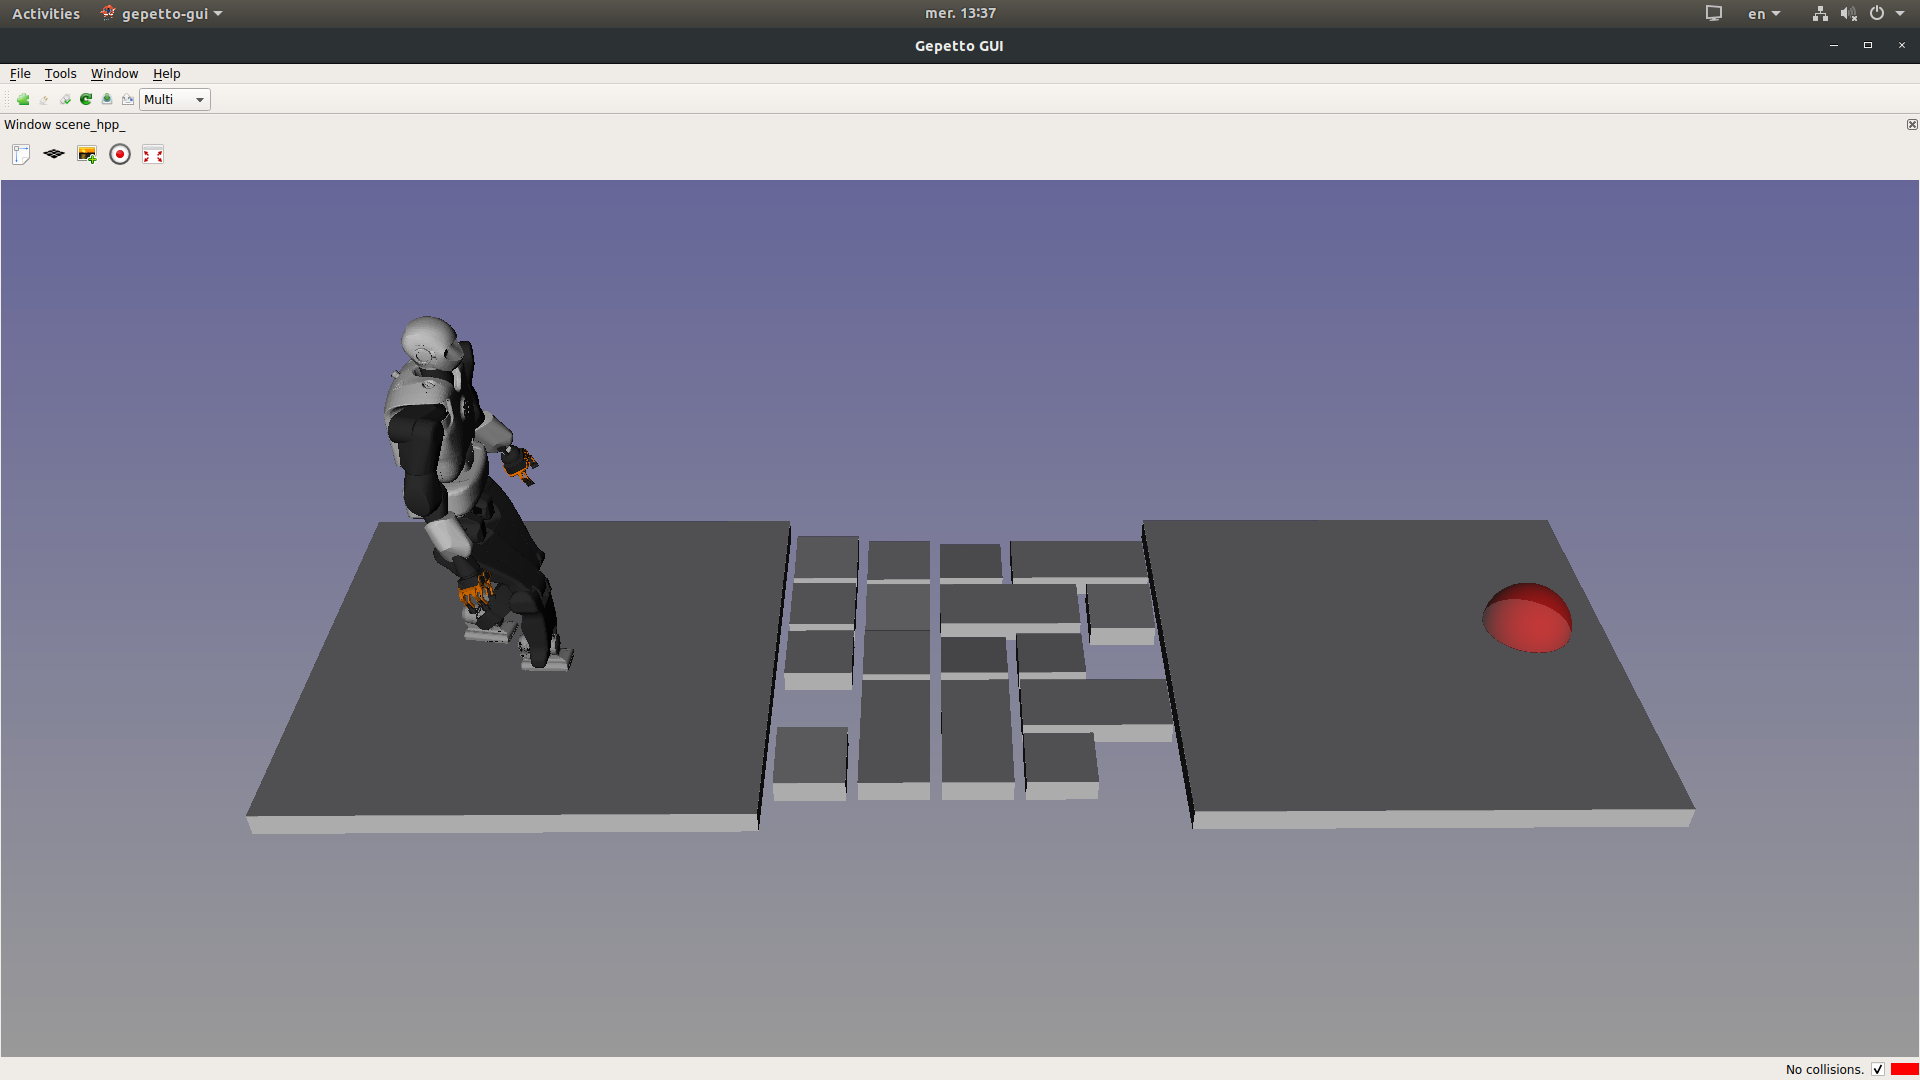
\includegraphics[trim={8cm 7cm 7.5cm 9cm},clip,width=0.8\textwidth,height=4cm]{Figures/Chapter_MIP_SL1M/rubbles/rubbles_empty.png}
    \caption{Given the desired number of steps $n$ and the set of candidate surfaces $\mathcal{S}$ (grey), the contact planner has to select the surfaces the robot has to step on, along with its foot placements on it to reach the objective area (red).\label{fig:rubbles:empty}}
\end{figure}

In this chapter, we will use two contact planners formulated with a Mixed-Integer Programming (MIP) approach.
%we plug our steering method LEAS into two contact planners with a Mixed-Integer Programming (MIP) approach.

%\textcolor{red}{Steve: il manquait une intro et dire pourquoi on utilise ces contact planners.}
%\textcolor{blue}{J'ai ajouté la phrase d'en dessous, qui mérite surement d'être revue.}

The sampling contact planner presented in previous section relies on heuristics to search for contacts in the robot environment.
While it can efficiently solve the contact planning problem, its sampling approach can not guarantee its completeness.
On the other hand, optimization-based approaches are an appealing approach to solve this limitation. However, they have to handle both the discrete choice of contact surfaces and the continuous optimization of placing contacts on them.
Previous works on contact planning \cite{deits2014FootPlanMI, sl1m_v2} solved this problem using a MIP approach or its relaxed form respectively.
We will explain both approaches and further investigate if our method LEAS can improve them through its guide paths generation.
%such contact planners have been used to solve both the discrete choice of selecting a sequence of surfaces to step on, and the continuous problem of placing contacts on these surfaces.

% What's the difference with the previous chapter
%The contact sequence generated by these contact planners does not follow exactly the guide path.
%Indeed, the guide path is used to collect the candidate surfaces along it.
%The contact planner then searches for a sequence of surfaces among these candidates as well as contact placement on it to reach a distant objective.
%Therefore, compared to SBCP presented in Chapter \ref{sec:CP-SB}, the steering methods have to solve a different set of limitations that we will explain later on.

% Chapter \ref{sec:CP-SL1M} investigates the use of LEAS plugged into a Mixed-Integer Programming contact planner and its relaxation \cite{sl1m_v2}. We explain the formulations of these contact planners and their limitations relative to the guide. Finally, we present the results as well as the different experiments we conducted.

This chapter is organized as follows:
Section \ref{sub:mip:notations} presents the notations used in this chapter.
Section \ref{sub:mip:mip} is an overview of the mixed-integer contact planner.
We will explain the advantage of using a guide path in this formulation, along with the issues it raises.
We then show how LEAS can learn to alleviate these limitations.
Section \ref{sub:mip:sl1m} explains the reformulation of the MIP into a feasibility linear program, called SL1M \cite{sl1m_v1}. 
We will present further insight into this reformulation, as well as the experiments conducted with LEAS to improve its convergence.

\section{Notations}
\label{sub:mip:notations}
Across this chapter, we use similar notations to the previous work \cite{sl1m_v2}.
\begin{center}
\begin{tabular}{ l l } 
    \hline
    \textbf{Notations} & \textbf{Description} \\ 
    \hline
    n                  & number of planned footsteps \\ 
    m                  & number of terrain contact surfaces \\ 
    $m_i$                & number of terrain contact surfaces for $i$-th footstep \\
    $\mathcal{S}$      & union of potential contact surfaces available \\
    $\mathcal{S}^j \subset \mathcal{S}$     & $j$-th contact surface \\
    $\mathcal{S}_i \subset \mathcal{S}$     & subset of $m_i$ contact surfaces considered in $i$-th footstep \\ 
    $\mathcal{S}_i^j \subset \mathcal{S}_i$ & $j$-th candidate contact surface in $i$-th footstep \\ 
    p$_i$              & $i$-th footstep position\\ 
    r$_i$              & $i$-th footstep orientation\\
    a$_i^j$            & integer slack variable for $j$-th surface in $i$-th footstep \\ 
    $\alpha_i^j$       & positive real slack variable for $j$-th surface in $i$-th footstep \\ 
    $\beta_i^j$        & real slack variable for $j$-th surface in $i$-th footstep \\
    %$card(a)$          & number of non-zero entries in vector $a$ \\
    $\mathcal{I}, \mathcal{G}$      & initial and goal constraint sets \\
    $\mathcal{F}$      & feasibility constraint set \\
    %\hline
    q              & virtual robot root configuration in $SE(3)$\\
    $H$              & local height map around the robot to get surface candidates\\
    \hline
\end{tabular}
\end{center}

%The terrain is represented as the union of $m$ surfaces $\mathcal{S}=\{\mathcal{S}^0,...,\mathcal{S}^m\}$ (Figure \ref{fig:rubbles:empty}).
The terrain is represented as the union of $m$ surfaces $\mathcal{S}= \bigcup_{j=1}^m \mathcal{S}^j$ (Figure \ref{fig:rubbles:empty}). 
Each contact surface $\mathcal{S}^j$ is a convex polygon in a 3D plane. 
For any foot position p$ \in \mathbb{R}^{3}$, we have:
\begin{equation}
\label{eq:p_in_S}
    \mbox{p} \in \mathcal{S}^j \iff  \mbox{p}^{\intercal} \mbox{d}^j = e^j \; \land \; S^j \mbox{p} \leq s_j 
\end{equation}
Where d$^j \in \mathbb{R}^3$ is the normal of surface $\mathcal{S}^j$, and $e^j \in \mathbb{R}$. The constant matrix $S^j \in \mathbb{R}^{h \times 3}$ and the vector $s^j \in \mathbb{R}^h$ define the $h$ half-spaces that bounds the surface $\mathcal{S}^j$.

For simplicity's sake, we denote $\mathcal{F}$ the set of dynamic and kinematic feasibility constraints. 
They guarantee the robot to follow the footstep plan in equilibrium without violating joint limits (Appendix \ref{appendix:feasibility_constr}).
In this work, we will formulate the initial constraint as $\mathcal{I} : \{\mbox{P}, \mbox{p}_1 = \mbox{p}_{\mathcal{I}}\}$, and the goal constraint as $\mathcal{G} : \{\mbox{P}, \mbox{p}_1 \in \mathcal{S}^{\mathcal{G}} \}$, where p$_{\mathcal{I}}$ is a constant and $\mathcal{S}^{\mathcal{G}}$ the destination surface.

% Paper SL1M v2: F denotes the set of kinematic and dynamic feasibility constraints that guarantee the robot to follow the footstep plan without falling or violating joint limits, detailed in an extended version of the present paper [30]

\section{Surface Selection and Contact Planning Problem}
\label{sub:mip:mip}

\subsection{Mixed-Integer Optimization}
% We are only interested in the feasibility problem. We will only briefly talk about the cost that we can optimize later.


We give the simplified contact planning problem as follows:
\begin{equation}
\label{eq:mip_simple}
\begin{aligned}
    \textrm{\textbf{find}}  \quad & \mbox{P}=[\mbox{p}_1,...,\mbox{p}_n], \;\mbox{p}_i \in \mathbb{R}^{3}\\
                            \quad & \mbox{R}=[\mbox{r}_1,...,\mbox{r}_n], \; \mbox{r}_i \in \mathbb{R}^{3}\\
    \textrm{\textbf{min}}  \quad & l(\mbox{P},\mbox{R})\\
    \textrm{\textbf{s.t.}}  \quad & \mbox{P} \in  \mathcal{I} \cap \mathcal{G} \cap \mathcal{F} \\
                            \quad & \mbox{p}_i \in \mathcal{S} \;\;\;\; \forall i, \; 1 \leq i \leq n
\end{aligned}
\end{equation}
We want to find a user-defined number $n$ of footsteps positions $p_i$ and orientations $r_i$, that minimizes an objective $l$(P,R).
The sequence $P$ and $R$ must satisfy some initial and goal conditions, $\mathcal{I}$ and $\mathcal{G}$, as well as the set of kinematic and dynamic feasibility constraints $\mathcal{F}$.
Finally, all foot positions p$_i$ must lie on a surface in $\mathcal{S}$.

As the condition p$_i \in \mathcal{S}$ is represented by inequality constraints(\ref{eq:p_in_S}), we can rewrite it as a Linear Programming (LP) problem using slack variables and the big M method \cite{big_M}:
\begin{align}
    \textrm{\textbf{find}}  \quad & \mbox{p}_i \in \mathbb{R}^3 \nonumber\\
                            \quad & \mbox{a}_i=[a_i^1,...,a_i^m], \; a_i^j \in \{0,1\} \nonumber\\
                            \quad & \beta_i=[\beta_i^1,...,\beta_i^m], \; \beta_i^j \in \mathbb{R} \nonumber\\
    \textrm{\textbf{s.t.}}  \quad & \mbox{card}(\mbox{a}_i) = m-1 \label{eq:cbm:surf:card}\\
                            \quad & \forall j \in \{1,..,m\} : \nonumber\\
                            \quad & \quad \quad S^j\mbox{p}_i \leq s^j + M a_i^j \textbf{1} \nonumber\\
                            \quad & \quad \quad (\mbox{p}_i)^{\intercal} \textbf{n}^j = e^j + \beta_i^j \nonumber\\
                            \quad & \quad \quad ||\beta_i^j||_1 \leq M a_i^j \nonumber\\
                            \nonumber
\end{align}
Where $\textbf{1}$ is a vector of appropriate size filled with ones.
We introduce the slack variables $a_i^j$ and $\beta_i^j$:
\begin{itemize}
    \item If $a_i^j = 0$, the corresponding surface $\mathcal{S}^j$ is selected and the $i$-th foot position $\mbox{p}_i$ lies on it, thus implying that $\beta_i^j = 0$.
    \item If $a_i^j = 1$, the constraints relative to the surface $\mathcal{S}^j$ always have a solution and can be ignored.
\end{itemize}
The big-M method introduces a sufficiently large scalar $M$ to solve our problem, but small enough to not hinder its convergence \cite{big_M_danger}.
The cardinality function (\ref{eq:cbm:surf:card}) counts the number of non-zero entries in a vector. 
It enforces the foot position p$_i$ to lie on exactly one surface in $\mathcal{S}$.

\paragraph{Contact-before-motion formulation.\label{par:cbm:formulation}}
We present the mixed-integer formulation for contact planning without guide (contact-before-motion) from \cite{sl1m_v2}, originally introduced by Deits et al. \cite{deits2014FootPlanMI}:
\begin{align}
    \textrm{\textbf{find}}  \quad & \mbox{P}=[\mbox{p}_1,...,\mbox{p}_n], \;\mbox{p}_i \in \mathbb{R}^{3} \nonumber\\
                            \quad & \mbox{R}=[\mbox{r}_1,...,\mbox{r}_n], \; \mbox{r}_i \in \mathbb{R}^{3} \nonumber\\
                            \quad & \mbox{A}=[\mbox{a}_1,...,\mbox{a}_n], \; \mbox{a}_i \in \{0,1\}^{m} \nonumber \\
                            \quad & \beta=[\beta_1,...,\beta_n], \; \beta_i \in \mathbb{R}^{m} \nonumber\\
    \textrm{\textbf{min}}  \quad & l(\mbox{P},\mbox{R}) \nonumber\\
    \textrm{\textbf{s.t.}}  \quad & \{\mbox{P},\mbox{R}\} \in \mathcal{I} \cap \mathcal{G} \cap \mathcal{F} \nonumber\\
                            \quad &\mbox{p}_n \in \mathcal{S}^{goal} \nonumber\\
                            \quad & \forall i \in \{1,..,n\} : \nonumber\\
                                \quad & \quad \mbox{card}(\mbox{a}_i) = m-1 \label{eq:cbm:mip_complete:card}\\
                                \quad & \quad \forall j \in \{1,..,m\} : \nonumber\\
                                    \quad & \quad \quad S^j\mbox{p}_i \leq s^j + M a_i^j \textbf{1} \nonumber\\
                                    \quad & \quad \quad (\mbox{p}_i)^{\intercal} \textbf{n}^j = e^j + \beta_i^j \nonumber\\
                                    \quad & \quad \quad ||\beta_i^j||_1 \leq M a_i^j \nonumber\\
                                    \nonumber
\end{align}

The cardinality constraints (\ref{eq:cbm:mip_complete:card}) enforce that exactly one surface $\mathcal{S}^j \subset \mathcal{S}$ is selected for each step.
We then consider the problem solved if all footsteps and cardinality constraints are respected.

Such a formulation can then be solved using a classical MIP approach, that is the LP-based branch-and-bound algorithm to handle the combinatorics (here the discrete surface selection) \cite{gurobi_mip}.
Finally, it is important to note that state-of-the-art MIP solvers, such as Gurobi \cite{gurobi}, have implemented additional methods to improve the solving efficiency such as presolvers \cite{presolve_gurobi_2020}, cutting planes \cite{cutting_plan_gomory_1996} and various heuristics. 

%\paragraph{Solving the Mixed-Integer Program.\label{par:mip:cbm:branchbound}}
%Such a formulation can then be solved using a classical MIP approach, that is the LP-based branch-and-bound algorithm \cite{gurobi_mip}.
%\begin{enumerate}
%    \item Relaxation of the slack variables. 
%    This step removes the integrality constraint on the slack variables $a_i^j$. 
%    As a result, the MIP is relaxed into a linear program problem that can be solved using the simplex algorithm \cite{simplex_history_1990}.
%    \item Tree expansion. If the result of the relaxed LP problem satisfies all integrality constraints, then our solution is optimal and we stop. Otherwise, two MIP sub-problems are derived from the relaxed solution and added to a search tree.
%\end{enumerate}
%Those steps are repeated for each MIP sub-problems until finding the optimal solution.
%Branch-and-bound can be seen as the exploration of the combinatorics between candidates surfaces for each step.
%In order to accelerate the solving of such an MIP problem, the problem can be reformulated so that the relaxation converges satisfies integrality constraints. 
%This approach will be covered with the contact planner SL1M \cite{sl1m_v1} in the next section.
%Finally, it is important to note that state-of-the-art MIP solvers, such as Gurobi \cite{gurobi}, have implemented additional methods to improve the solving efficiency such as presolvers \cite{presolve_gurobi_2020}, cutting planes \cite{cutting_plan_gomory_1996} and various heuristics. 
%Those methods will be used to speed up the solving.

% Mini conclu
\paragraph{Contact-before-motion formulation analysis.}
This formulation can explore all terrain contact surfaces in $\mathcal{S}$ while optimizing footstep positions and orientations on them.
As a result, it offers a guarantee of completeness under the problem constraints.

However, in most scenarios such as Figure \ref{fig:rubbles:empty}, we can not know other than empirically how many steps $n$ are required to reach the distant objective.
The tuning of the number of steps $n$ is avoided in \cite{deits2014FootPlanMI} by defining a maximum bound for the required number of steps. The MIP problem is then solved with a cost encouraging the robot to reach the goal with the minimum number of steps. 
Once done, the redundant footsteps in the goal area are then discarded.
A critical limitation of this approach is the manual tuning of the maximum number of steps. 
On the one hand, overestimating this number results in unnecessary computation due to the number of redundant footsteps.
On the other hand, underestimating it can make the problem infeasible.

Overall, as the number of steps $n$ and candidate surfaces $m$ increase, so do exponentially the dimension and complexity of the problem ($n^m$). As a consequence, this method can result in contact planning times up to several seconds for a few steps.


\subsection{Advantages of the Guide Path and Problem Statement}
%\begin{figure}[ht]
%    \centering
%    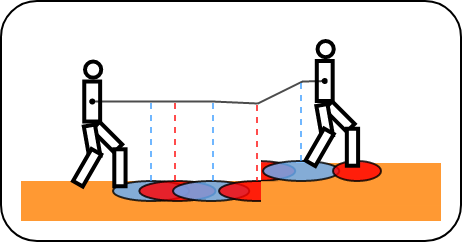
\includegraphics[width=0.7\textwidth, height=5cm]{Figures/Chapter_MIP_SL1M/strategies_cp_guide_B.png}
%    \caption{Given root configurations along the guide path, the contact planner computes the reachable surfaces to step on and optimizes the contact placements on it.}
%    \label{fig:cp-sb:strategy_cp-sb}
%\end{figure}
In order to fix the limitations of tuning the number of steps $n$ as well as the problem complexity, we can reformulate the MIP formulation with a motion-before-contact approach, i.e. using a guide path.

\begin{figure}[h!]
    \centering
    \captionsetup[subfigure]{justification=centering}
    \begin{subfigure}[t]{0.7\linewidth}
        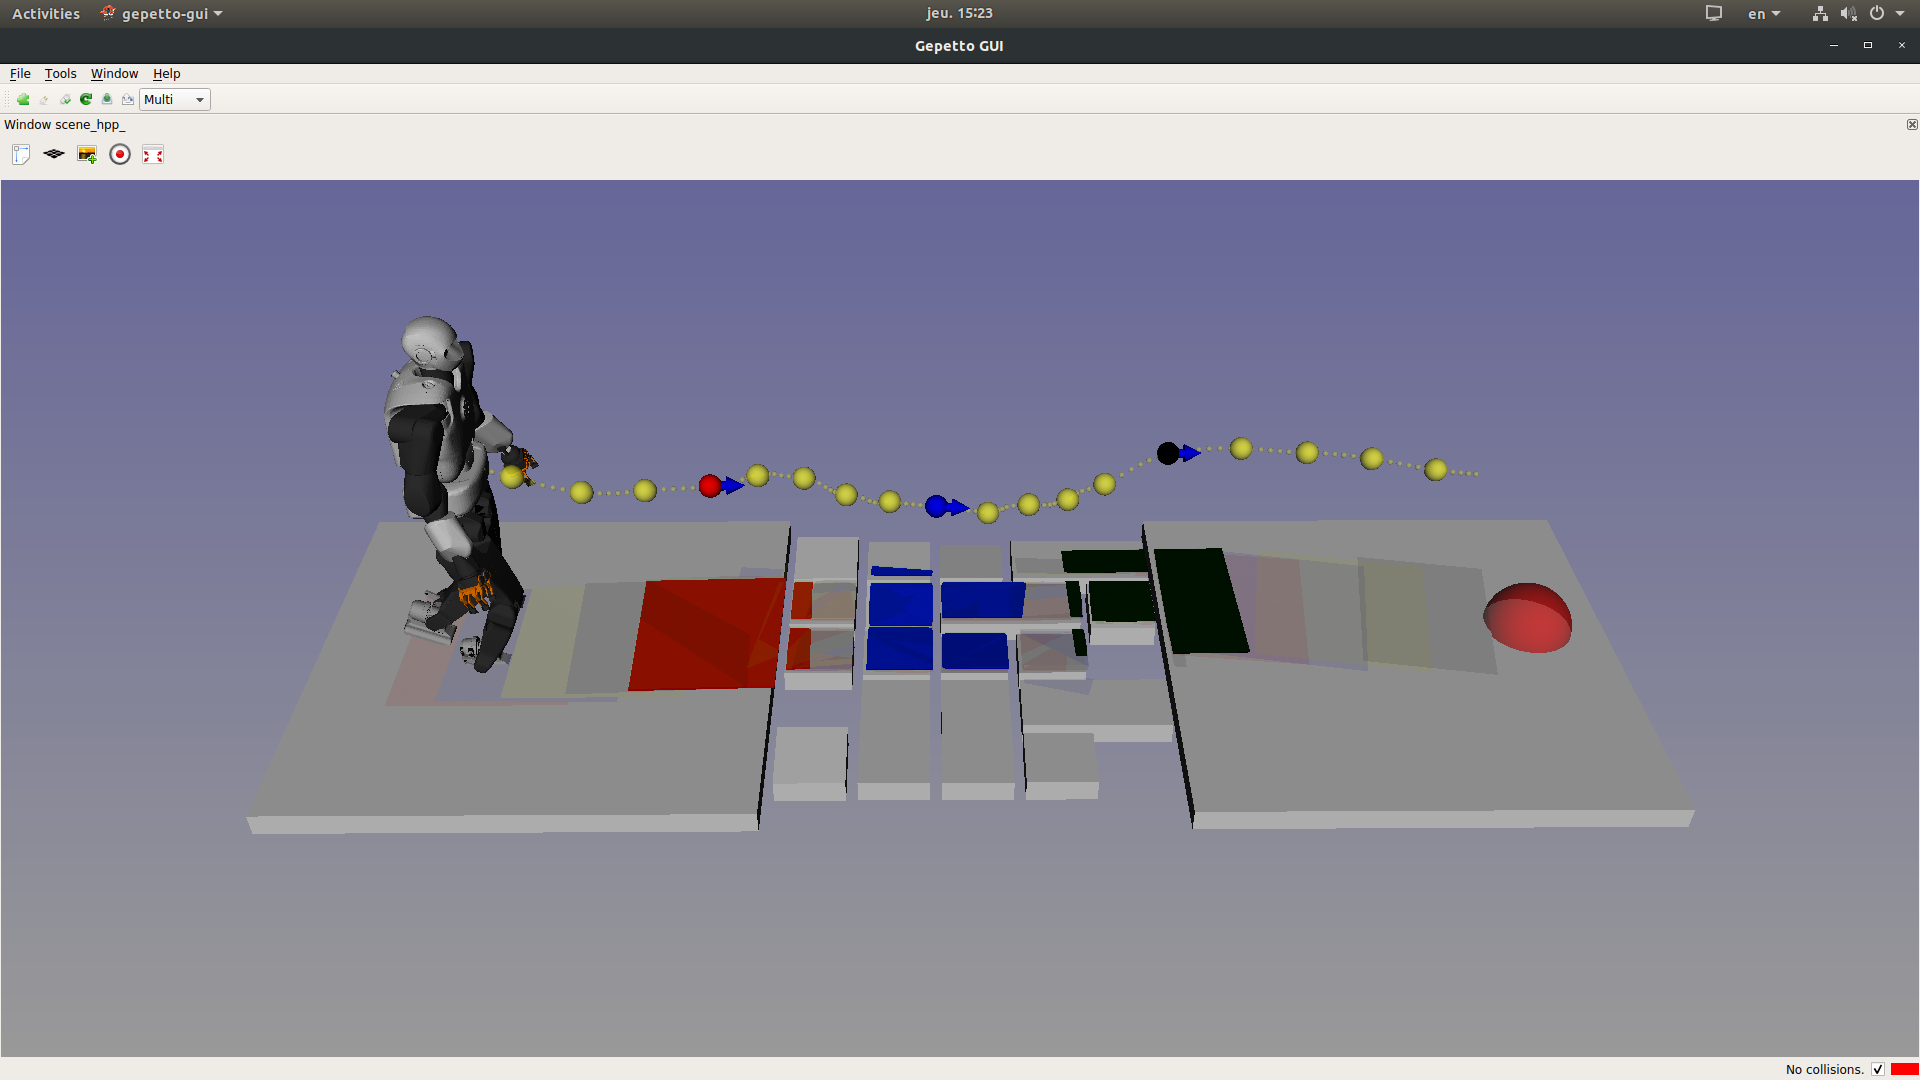
\includegraphics[trim={10cm 8cm 10cm 10cm},clip,width=\textwidth,height=4cm]{Figures/Chapter_MIP_SL1M/rubbles/rubbles_steps_4_9_14.png}
        \caption{Guide path planning and candidate surfaces\label{fig:rubbles:surf_sel_0}}
    \end{subfigure}
    \begin{subfigure}[t]{0.7\linewidth}
        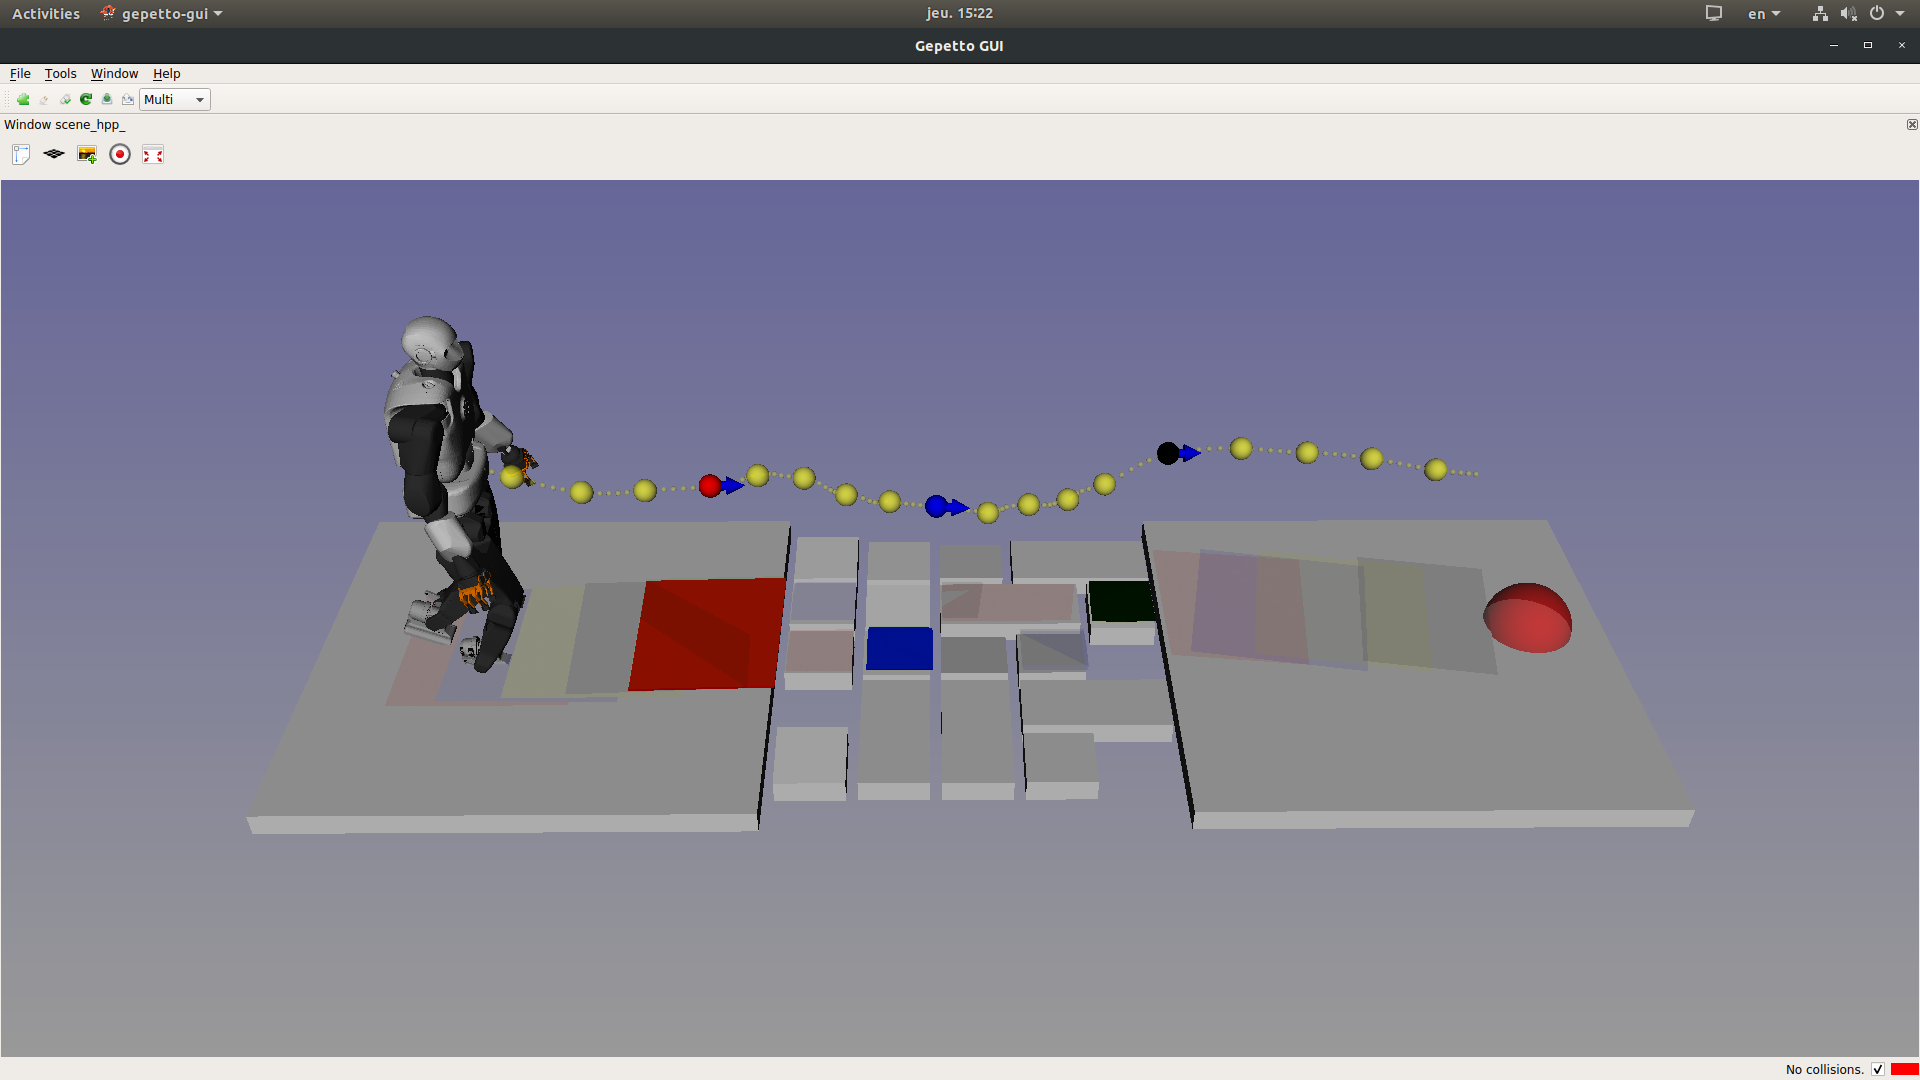
\includegraphics[trim={10cm 8cm 10cm 10cm},clip,width=\textwidth,height=4cm]{Figures/Chapter_MIP_SL1M/rubbles/rubbles_steps_4_9_14_selected.png}
        \caption{Contact surface selection\label{fig:rubbles:surf_sel_1}}
    \end{subfigure}
    \begin{subfigure}[t]{0.7\linewidth}
        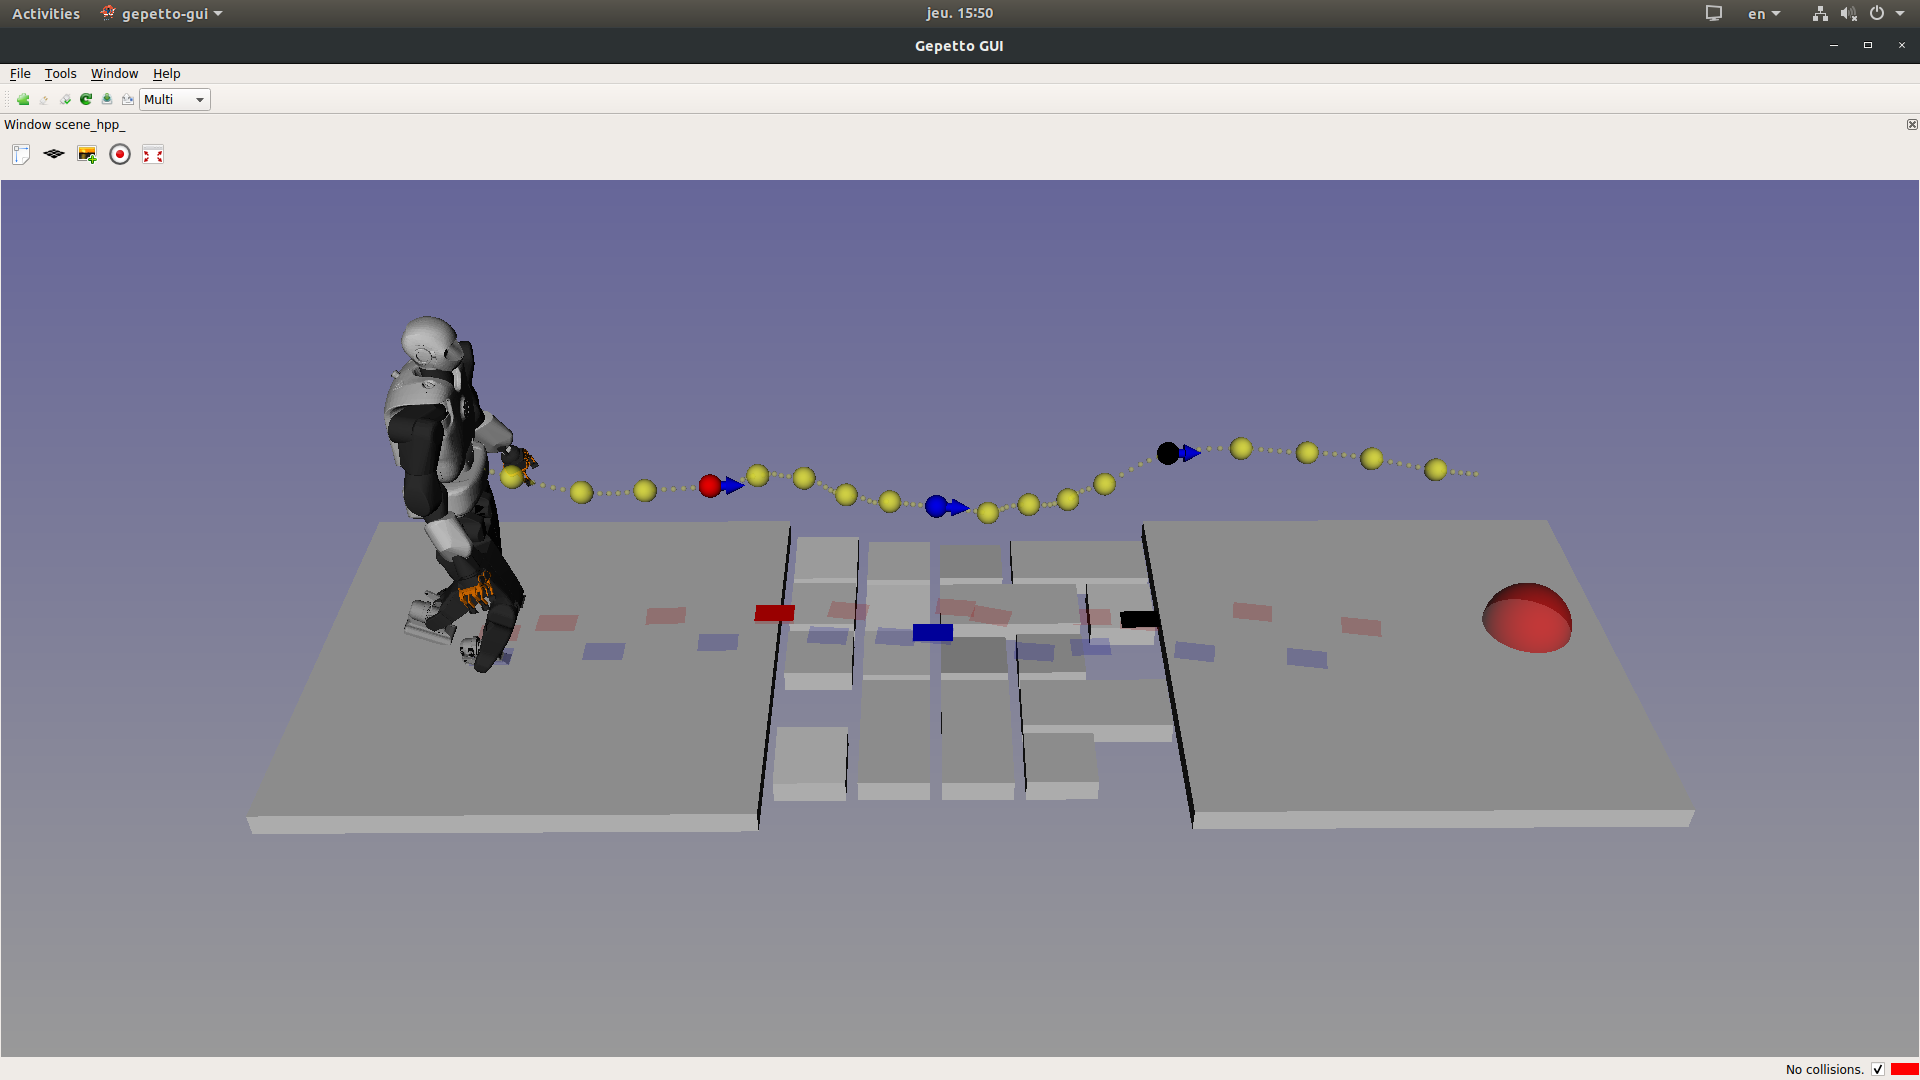
\includegraphics[trim={10cm 8cm 10cm 10cm},clip,width=\textwidth,height=4cm]{Figures/Chapter_MIP_SL1M/rubbles/rubbles_steps_4_9_14_steps.png}
        \caption{Contact placement\label{fig:rubbles:surf_sel_2}}
    \end{subfigure}
    \caption{MIP with guide path: (a) the steering method plans a guide and get a reduced set of candidate surfaces for each step, (b) the contact planner selects the surfaces to step on, and (c) it places the contacts on it. We highlight three configurations for better visualization.\label{fig:rubbles:surf_sel}}
\end{figure}


% Show the results obtained in SL1M V2?
% Compare the results?

\paragraph{Motion-before-contact formulation.\label{par:mip:mbc:formulation}}
We explain the mixed-integer approach from Song et al. \cite{sl1m_v2} using a guide path. 
The formulation is as follows:
\begin{align}
    \textrm{\textbf{given}} \quad & \mbox{R}=[\mbox{r}_1,...,\mbox{r}_n], \; \mbox{r}_i \in \mathbb{R}^{3} \label{eq:mbc:mip_complete:rotation}\\
                            \quad &\mathcal{X}=[\mathcal{S}_1, ..., \mathcal{S}_n] \label{eq:mbc:mip_complete:surf_pruned}\\
    \textrm{\textbf{find}}  \quad & \mbox{P}=[\mbox{p}_1,...,\mbox{p}_n], \;\mbox{p}_i \in \mathbb{R}^{3 \times n} \nonumber\\
                            \quad & \mbox{A}=[\mbox{a}_1,...,\mbox{a}_n], \; \mbox{a}_i \in \{0,1\}^{m_i} \nonumber \\
                            \quad & \beta=[\beta_1,...,\beta_n], \; \beta_i \in \mathbb{R}^{m_i} \nonumber\\
    \textrm{\textbf{min}}  \quad & l(\mbox{P},\mbox{R}) \nonumber\\
    \textrm{\textbf{s.t.}}  \quad & \{\mbox{P},\mbox{R}\} \in \mathcal{I} \cap \mathcal{G} \cap \mathcal{F} \nonumber\\
                            \quad & \forall i \in \{1,..,n\} : \nonumber\\
                                \quad & \quad \mbox{card}(\mbox{a}_i) = m_i-1 \nonumber \\
                                \quad & \quad \forall j \in \{1,..,m_i\} : \label{eq:mbc:mip_complete:surf_cand}\\
                                    \quad & \quad \quad S_i^j\mbox{p}_i \leq s_i^j + M a_i^j \textbf{1}  \nonumber\\
                                    \quad & \quad \quad (\mbox{p}_i)^{\intercal} \textbf{n}^j = e^j + \beta_i^j \nonumber\\
                                    \quad & \quad \quad ||\beta_i^j||_1 \leq M a_i^j \nonumber\\
                                    \nonumber
\end{align}

\paragraph{Simplification of the problem.}
\begin{figure}[h!]
    \centering
    \captionsetup[subfigure]{justification=centering}
    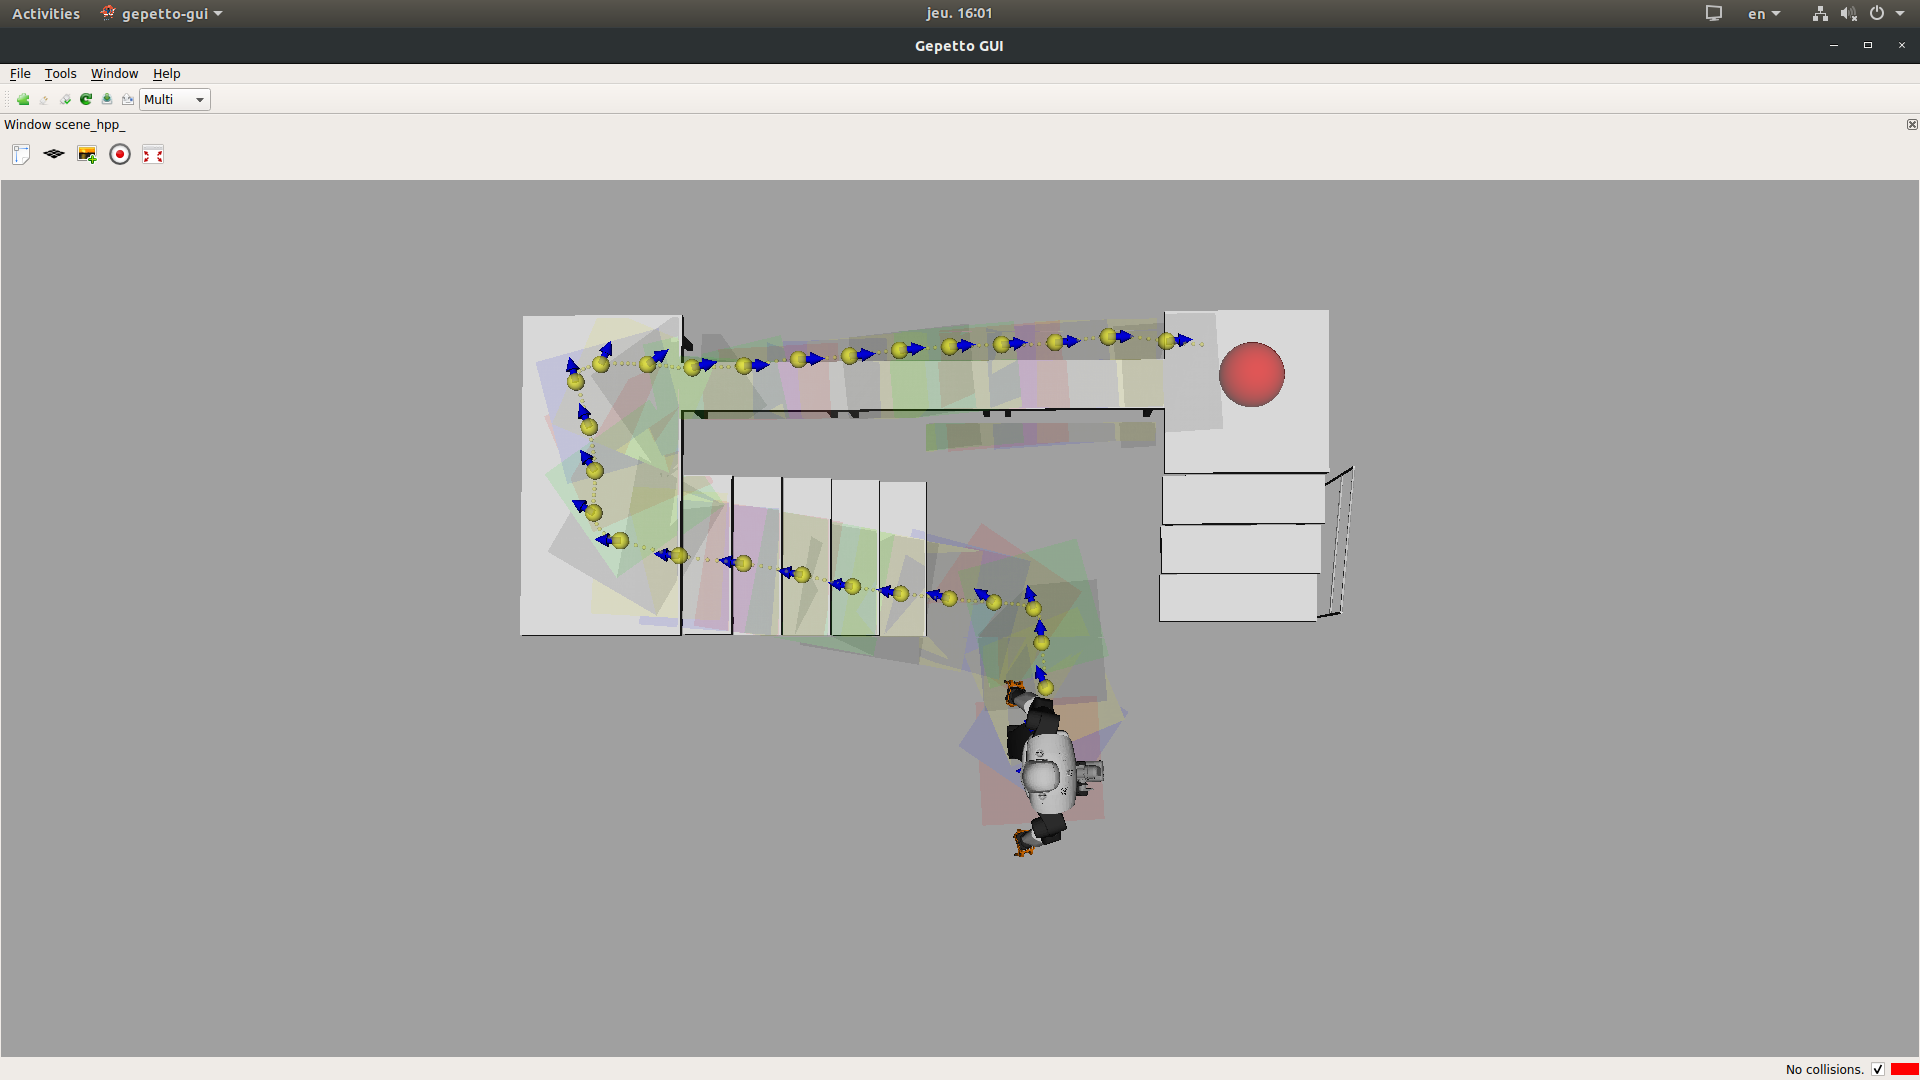
\includegraphics[trim={15cm 5cm 18cm 7cm},clip,width=0.8\textwidth,height=7cm]{Figures/Chapter_MIP_SL1M/bauzil_guide_surfaces.png}
    \caption{Guide path for surface selection: (yellow) robot root configurations discretized on the guide path, (blue) orientation of the root, (colored rectangles) the candidate surfaces around the root.\label{fig:mip:bauzil_guide_surfaces}}
\end{figure}
As shown on Figure \ref{fig:mip:bauzil_guide_surfaces}, each discretized robot root configuration $\mbox{q}_i$ along the guide gives several information. As a result, they can be used to simplify the previous formulation.

% Guessing the number of footsteps.
The number of steps $n$ can be deduced from the guide path.
Indeed, the guide paths can be discretized to obtain a desired discretization $\Delta D$ between each root configuration $\mbox{q}_i$.
Contrary to the contact planner presented in the previous chapter, one step is made with a cyclic gait for each discretized root configuration along the guide.

% Constraining the feet orientation.
The footsteps orientation can follow the robot root orientation (blue arrows in Figure \ref{fig:mip:bauzil_guide_surfaces}).
With this approach, the rotation sequence R can directly be given as input (\ref{eq:mbc:mip_complete:rotation}), thus drastically reducing the dimension of the problem.

% Pruning irrelevant contact surfaces
The candidate surfaces for each step $\mathcal{S}_i$ can be pruned to reduce the search space around a discrete root location along the guide.
We give as input the sequence $\mathcal{X}$, in which we associate to each footstep their corresponding candidate surfaces subset $\mathcal{S}_i$ (\ref{eq:mbc:mip_complete:surf_pruned}). Each subset contains $m_i$ surfaces with $m_i \leq m$. 
As a result, the number of candidate surfaces explored in the problem are lesser (\ref{eq:mbc:mip_complete:surf_cand}), as well as the number of slack variables in a$_i$ and $\beta_i$.
It is important to note that if the $i$-th step has only one surface candidate ($m_i=1$), the corresponding slack variable value can be fixed: $a_i^1 = 0$.

% Phrase de steve: The guide path is used to pre-filter the non-relevant contact surfaces. Informally, for a discrete root location along the guide path, the reachable workspace of the robots is used to discard any surface that is not in the neighbourhood of the robot. => Je n'utilise pas vraiment le reachable workspace donc je n'ai pas mis la phrase.

\paragraph{Previous results.}
In the previous work \cite{sl1m_v2}, Song et al. use RB-Kino with RRT \cite{kinodynamic_sm_2017} presented in the previous chapter to generate guide paths.
Their results demonstrate the computation time advantage of using a guide path in this formulation. 
Furthermore, they accelerate the contact planning by solving separately a feasibility problem (i.e. without $l(\mbox{P},\mbox{R})$) to obtain the surfaces to step on, then optimize the footstep placements on them with a quadratic cost (i.e. with $l(\mbox{P},\mbox{R})$).
As a result, their algorithm can plan a few steps in tens of milliseconds using the commercial solver Gurobi \cite{gurobi}.

\paragraph{Problem statement.}
% How to discretize the guide ?
The main limitation of this approach is the tuning of the discretization steps $\Delta D_i$ for each step $i$ along the guide path (i.e. distance between each root configuration).

In the previous work \cite{sl1m_v2}, the average value $\Delta\overline{D}$ is manually tuned to fit a given scenario.
But as stated in their discussion, if this value is too large (i.e. a small number of footsteps $n$), the problem can become unfeasible. Conversely, a too small value can lead to redundant footsteps and increase the problem dimension.
Trivially, we can expect the contact planning to succeed on flat ground for the Talos robot with a $\Delta\overline{D} \approx 25$ cm, that is the near maximum step length of the robot. However, lowering it when crossing more complex terrains is required to ensure planning feasibility.

That is why it is desirable to automatically tune $\Delta D_i$ along the guide depending on the terrain traversed, as previously discussed in Chapter \ref{sec:CP-SB}.
Implementing some heuristics to solve this problem can be difficult. Indeed, they have to evaluate the terrain traversability and estimate the next suitable discretization step.
We thus give the following question: \textit{what is the maximum discretization step feasible by the contact planner for a given terrain?}
Answering this question could reduce the number of steps in the MIP problem, thus lowering its complexity, while ensuring its feasibility.
%Moreover, it also solves the limitation of the contact-before formulation.

% What is the range of surfaces around the robot we should give ?
% Is there an impact about the path taken ? => No, not with our formulation

\subsection{Implementation Details}
\label{subsub:mip:implementation_details}
Our goal is to adapt the discretization steps $\Delta D_i$ for each step along guide paths depending on the traversed terrain.
The number $n$ of discretized configurations $\mbox{q}_i$ on the guide must then produce feasible problems for the contact planner.
To do so, we use our steering method LEAS to generate such guide paths by adapting its velocity, hence the $\Delta D_i$ values along.

In this work, we use Gurobi solver \cite{gurobi} with its presolver and heuristics to solve the MIP formulation for contact planning (Section \ref{par:mip:mbc:formulation}).

\paragraph{RL policy.}
We employ the exact same network architecture, actions, rewards, and hyperparameters as described in chapter \ref{sec:LEAS}. We set the number of asynchronous workers computing contacts with the MIP planner to 6.
To help LEAS estimate the terrain traversability, we add a scalar to the states that represents the number of reachable surfaces around the robot.

Our method LEAS takes as input the local height map of the terrain $H$, the direction to the goal, and the number of surfaces around the robot to locally navigate the terrain. 
The methodology is similar to Chapter \ref{sec:CP-SB}.
States generated by LEAS are subject to some reachability $\tilde{\mathcal{R}^*}$ and collision-free $\tilde{\mathcal{C}}$ conditions (see Chapter \ref{sec:LEAS}), plus the additional constraint that is to succeed the guide path with the MIP contact planner.

%\paragraph{Contact planner parameters.}
% Value of M? bof
% There is none in fact.

\paragraph{Candidate surfaces.}
% We get the surfaces in a square around the robot directly from the heightmap => Faster than computing the intersection of ROM with the terrain surfaces.
% Parameters used compared to LEAS and SL1M + discretization etc.
% I have two modes: PBP and MPC.
We obtain candidate surfaces $S_i$ from the local height map $H_i$ around the robot configurations $\mbox{q}_i$ (colored rectangles in Figure \ref{fig:mip:bauzil_guide_surfaces}).
We choose this method as we can easily get such an height map with our implementation, but any other method to obtain candidate surfaces around the robot could be applied.

The small size of the height map (80x80 cm) may lower the number of candidate surfaces and so the feasibility of the problem. 
%\stn{why} \textcolor{blue}{J'ai ajouté que ça réduisait le nombre de candidat, il en faut plus ou pas?}
However, it also constrains the footstep placements in the guide vicinity, as well as lowering the problem complexity by reducing the number of candidate surfaces.
We will further discuss this implementation choice and its alternatives in Section \ref{subsub:mip:discussion:candidate_surfaces}.

It is important to note that compare to the sampling contact planner of the previous section, the MIP planner generates contact sequences that do not follow exactly the guide.
While the root trajectory could be used as a part of the cost to optimize, in this work, it is solely used to collect candidate surfaces along it.


\paragraph{Discretization of the guide.}
The discretization of the guide generated by LEAS corresponds to an average of $\Delta \overline{D}=2$ cm between each configuration (See Chapter \ref{sec:LEAS}). Indeed, the desired velocity $v_{desired}=0.10$ m/s and the fixed timestep $T=0.2$ s results in an average: $\Delta \overline{D} = v_{desired} \times T = 2$ cm.

With the MIP contact planner, a footstep is made for each discretized configuration along the guide.
Our goal is to get a sufficiently high discretization step $\Delta D_i$ for each step along the guide, in order to lower the contact planning complexity while ensuring its feasibility by the contact planner.

In this chapter, we aim for a maximum $\Delta \overline{D} =28$ cm. 
This value corresponds to the near maximum step length that the Talos robot could possibly perform.
To do so, we further discretize the guide in the input of our MIP contact planner by only keeping 1 out of $N_{ref}=14$ configurations on it.
Depending on the terrain, LEAS may not be able to generate feasible guide paths with this maximum value (i.e. navigate the terrain at the desired velocity).
As a result, LEAS has to learn how to adapt the robot root velocity and implicitly $\Delta D_i$ along the guide to succeed in the contact planning.


\paragraph{Contact planning choices.}

In this thesis, we focus on solving a feasibility problem without quadratic cost, i.e. $l(\mbox{P},\mbox{R})=0$.
%This implementation choice is motivated by the fact that if a solution to the problem exists, it can be optimized later on \cite{sl1m_v2}.
This implementation choice is motivated by the fact that we want to avoid the high computation time spent by the MIP solver on optimizing this cost.
however, once one surface is assigned to each footstep, a new problem with this cost can be solved with a faster quadratic solver, but at the cost of optimality.
% with the branch-and-bound algorithm. %The footsteps can be further optimized after solving the surface selection problem, however at the cost of optimality.

The MIP formulation selects surfaces and optimizes feasible foot placements on it for all footsteps simultaneously.
As a consequence, the contact planner can not return the last successful step along the guide, contrary to the sampling-based contact planner of the previous section.
In order to train LEAS with feedback from the contact planner as described in Chapter \ref{sec:LEAS}, two different methods can be used.

The first strategy is a Dichotomic Search to obtain the last successful step on the guide path with the contact planner. 
It is a long-horizon approach, and so guarantees the completeness of the contact planning up to the last successful step. %However, as the length of the path increases, the dichotomic search can also increase the computation time during the training. 
%In practice, the feasibility problem is solved fast enough, and so the additional computation time is tolerable even for tenths of footsteps.

The second strategy is to plan contacts in a model-predictive control fashion such as \cite{fanny_mip_solo}. 
To do so, they generate a short guide path, then solve the contact planning for $n$ steps (with $n$ a small number).
They then keep the first step generated and repeat the process.
The algorithm stops when the goal is reached or the contact planning fails.
This strategy is a short-horizon approach, and thus alleviates the combinatorics aspect of the problem. 
However, it is prone to local minima.
%Indeed, solving the contact planning problem section by section instead of solving the complete problem at once lowers its likelihood to be feasible.
This limitation is avoided in their implementation by solving the problem with a regularization cost in $l(\mbox{P},\mbox{R})$, but at the cost of a longer computation time than a feasibility problem.

In this work, we want to avoid adding such costs for computation efficiency purposes. 
Moreover, short-horizon planning can not guarantee completeness, which is not desirable for our task.
That is why, we choose the first strategy, solving the long-horizon contact planning problem along the whole guide path.

%The contact planner then searches for a sequence of surfaces among these candidates as well as contact placement on it to reach a distant objective.
%Therefore, compared to SBCP presented in Chapter \ref{sec:CP-SB}, the steering methods have to solve a different set of limitations that we will explain later on.


\paragraph{Training.}
\begin{figure}[t]
    \centering
    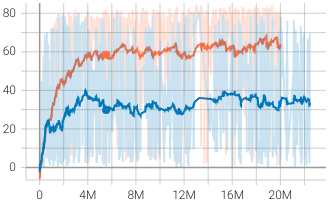
\includegraphics[trim={0 0 0 0},clip,width=0.6\textwidth]{Figures/Chapter_MIP_SL1M/learning_curve_MIP_P1.png}
    \caption{Learning curves of (red) LEAS-P1 trained without contact planner and (blue) LEAS-P2 trained with feedback from the MIP contact planner.}
    \label{fig:mip:learning_curves}
\end{figure}
We train LEAS with feedback from the MIP contact planner on the training terrain presented in Chapter \ref{sec:LEAS}.
The model is evaluated after 12 million steps corresponding to 8 hours of training on a PC with an Intel Core i7-8700 (12 cores, 3.20Ghz, 16GB ram). 

Learning curves of LEAS without contact planner, referred as LEAS-P1, and LEAS-P2 with the MIP contact planner are shown in Figure \ref{fig:mip:learning_curves} (the maximum reward is equal to 100 for trajectories in a straight line).
%The P2 validation increases its probability to meet a terminal condition (i.e. failing the contact planning) and forces LEAS to adapt its behavior to succeed with the contact planner, resulting in a lower average reward per episode.
The episode rewards of LEAS-P2 are lower than LEAS-P1 due to the contact planning constraints. 
As described earlier, we discretize the guide so that when moving at the desired velocity $v_{desired}=0.10$ m/s, the discretization step is equal to $\Delta D=28cm$. 
This value is at the limit of the feasibility constraints $\mathcal{F}$ (Appendix \ref{appendix:feasibility_constr}) of the TALOS robot on flat ground. 
Consequently, our steering method has to move the robot root slower to succeed in the contact planning on more complex terrains, thus resulting in a lower average reward.



\subsection{LEAS Results}
\label{subsub:mip:results}


% I trained with skip 15, but it's better to keep a margin => 14 works well, check the % of success.
% I also have 2 modes => PBP and MPC

% I will get all the results on 1x11 probably?
% Start oriented toward the goal with an initial velocity of 0.5
% I will not compare to Kino maybe? Does not make sense?

% Ok I will just do the experiment on the 1x11 I guess
% I check the percentage of success of the policy on this scene first, and how to use it. => See the margin
% Then I compare P1 vs P2, and their percentage of success (I have the tabs)
% Finally I can check if there is something to see on the plot vel, if in average he goes slower in some terrains compared to P1.
% For this one, 5 trajectories should suffice.
% So it's 2 results on the same scene.

We expect LEAS-P2 to find, depending on the terrain, some sufficiently high discretization steps $\Delta D_i$ along the guide with the parameter $N_{ref}$, that are feasible by the contact planner.
On difficult terrains such as rubbles and stairs, LEAS should lower the robot root velocity, and thus $\Delta D_i$, to ensure the contact planning success. 
On contrary, we expect the robot to move with a higher velocity on easy ones such as flat ground.

%We trained LEAS-P2 with the MIP contact planner by keeping 1 out of $N_{keep}=14$ configurations.

%However, the balance between the reward $R_{dir}$ to move in the desired direction at $v_{desired}$ and the constraint to succeed the contact planning forces LEAS-P2 to always work near the limits of what the contact planner can achieve.
%To better visualize the impact of the discretization of the guide, will compare the results of our steering methods for different values of $N_{keep}$ and so different discretization step $\Delta D$.

\paragraph{Basic scenarios.\label{subsub:mip:basic_scenarios}}
\begin{figure}[h!]
    \centering
    \captionsetup[subfigure]{justification=centering}
    \begin{subfigure}{0.9\linewidth}
        \centering
        \begin{subfigure}{0.48\linewidth}
            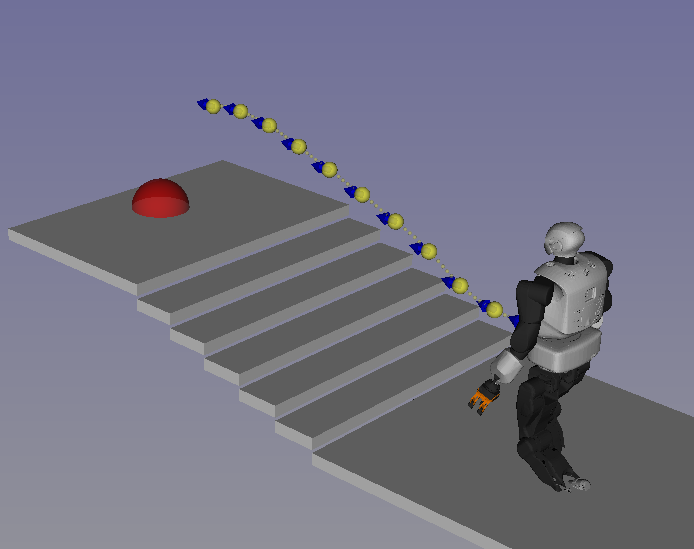
\includegraphics[trim={0cm 0cm 0cm 0cm},clip,width=\textwidth,height=4.5cm]{Figures/Chapter_MIP_SL1M/res_mip/scenario_stairs.png}
        \end{subfigure}
        \begin{subfigure}{0.48\linewidth}
            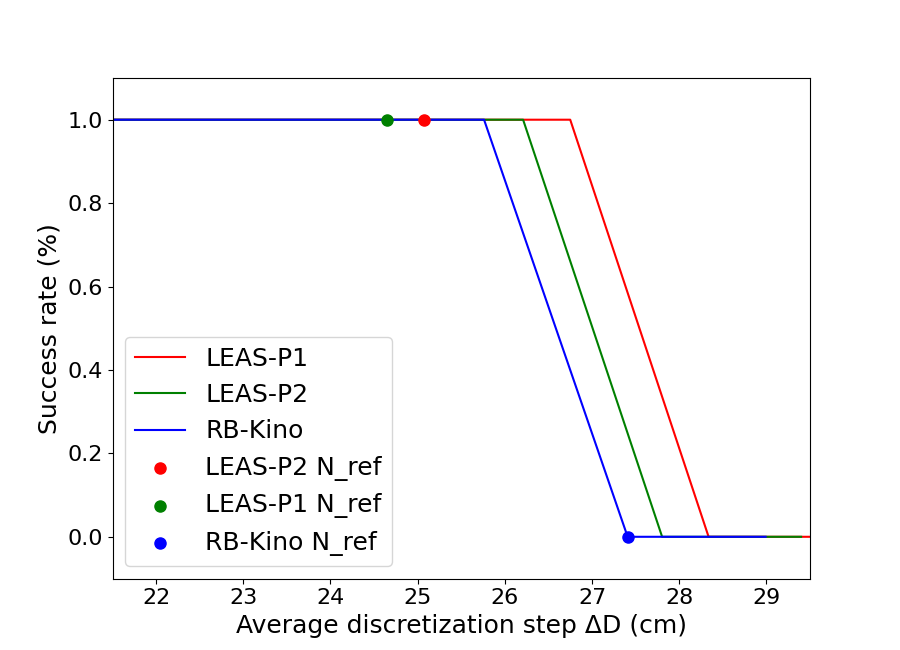
\includegraphics[trim={0cm 0cm 2cm 1.8cm}, clip,width=\textwidth,height=4.5cm]{Figures/Chapter_MIP_SL1M/res_mip/MIP_stairs/FIGURE_MIP_STAIRS_2.png}
        \end{subfigure}
        \caption{Stairs (up)}
        \label{fig:mip:minimizing_basic:0}
    \end{subfigure}
    \begin{subfigure}{0.9\linewidth}
        \centering
        \begin{subfigure}{0.48\linewidth}
            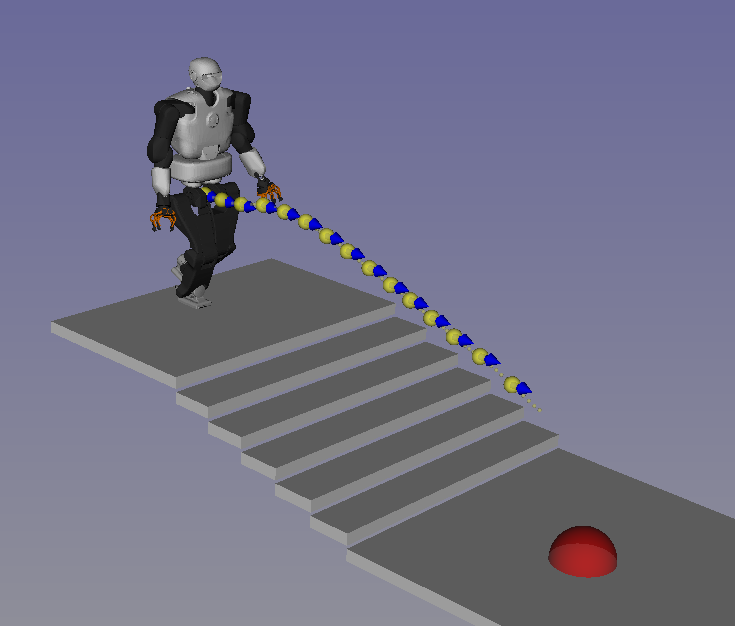
\includegraphics[trim={1cm 0cm 0cm 0cm},clip,width=\textwidth,height=4.5cm]{Figures/Chapter_MIP_SL1M/res_mip/stairs_down.png}
        \end{subfigure}
        \begin{subfigure}{0.48\linewidth}
            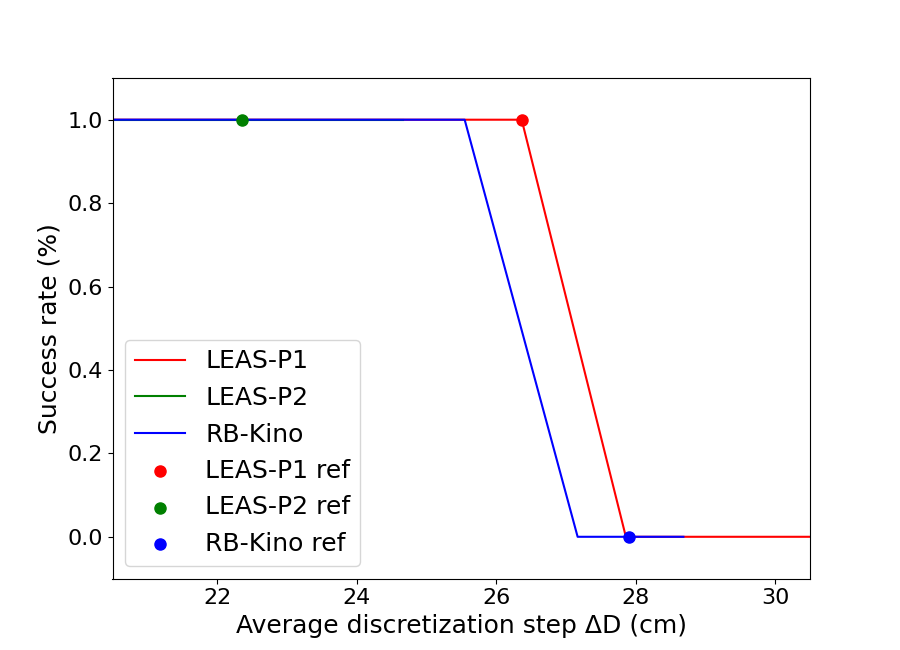
\includegraphics[trim={0cm 0cm 2cm 1.8cm}, clip,width=\textwidth,height=4.5cm]{Figures/Chapter_MIP_SL1M/res_mip/MIP_stairs/FIGURE_MIP_STAIRS_DOWN_2.png}
        \end{subfigure}
        \caption{Stairs (down)}
        \label{fig:mip:minimizing_basic:1}
    \end{subfigure}
    \begin{subfigure}{0.9\linewidth}
        \centering
        \begin{subfigure}{0.48\linewidth}
            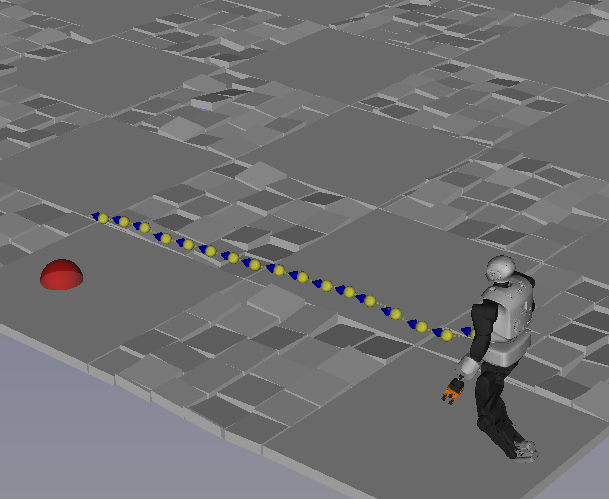
\includegraphics[trim={0cm 0cm 0cm 0cm},clip,width=\textwidth,height=4.5cm]{Figures/Chapter_MIP_SL1M/res_mip/scenario_rubbles.png}
        \end{subfigure}
        \begin{subfigure}{0.48\linewidth}
            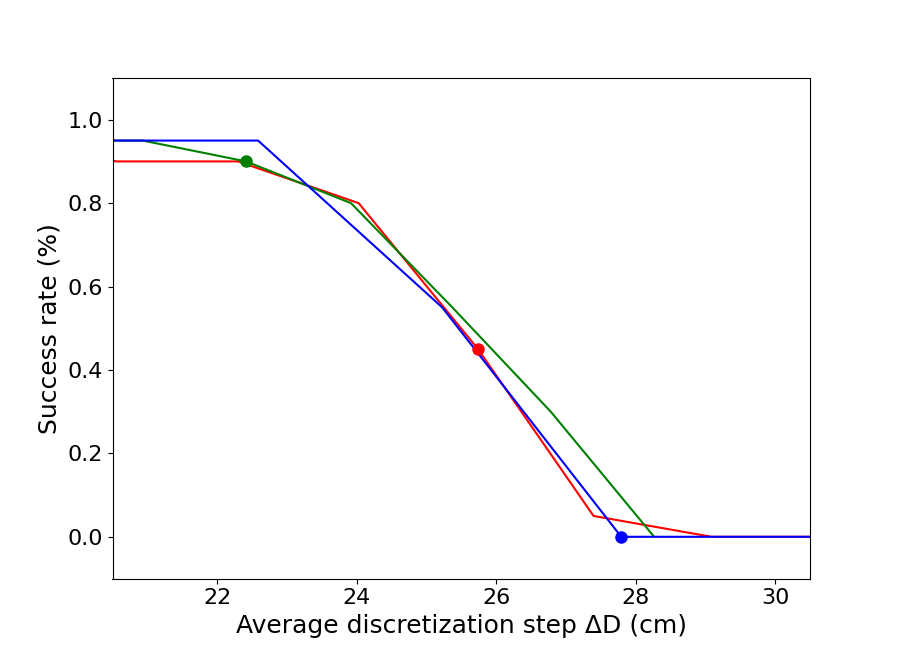
\includegraphics[trim={0cm 0cm 2cm 1.8cm}, clip,width=\textwidth,height=4.5cm]{Figures/Chapter_MIP_SL1M/res_mip/MIP_res_rubbles/FIGURE_MIP_RUBBLES_2.png}
        \end{subfigure}
        \caption{Rubbles}
        \label{fig:mip:minimizing_basic:2}
    \end{subfigure}
    \caption{Comparison of the steering methods success with MIP contact planning for different discretization steps. Colored dots correspond to results with the value $N_{ref}$ used across all scenarios.}
    \label{fig:mip:minimizing_basic}
\end{figure}
we will first show the impact of the average $\Delta \overline{D}$ value along the guide on the MIP contact planning success. 
It will permit us to evaluate the difficulty of our basic scenarios (stairs and rubbles on Figure \ref{fig:mip:minimizing_basic}). 

We compare the results of LEAS-P1, LEAS-P2, and RB-Kino.
For each scenario, the initial robot root is oriented toward the goal with a velocity $v_{init}=0.05$ m/s.
Each steering method acts on the root velocity to potentially reach the desired velocity $v_{desired}=0.10$ m/s, which corresponds to a discretization step $\Delta \overline{D}=28$ cm with $N_{ref}=14$ at the edge of the feasibility constraints $\mathcal{F}$ on flat ground.

We test our steering methods for different values of $N$, where we keep 1 out of $N$ configurations along the guide ($N \in \{8,20\}$), which permits to cover a wide range of discretization steps.
Indeed, increasing the $N$ value implies a higher average $\Delta \overline{D}$ along the guide and inversely.
Each $N$ value is tested on 30 trajectories per scenario.
We represent the result of the steering methods for $N=N_{ref}$ by some colored dots (the value LEAS-P2 has been trained on).

We can observe the success rate of the steering methods depending on their average discretization step for each scenario.
%The stairs scenario is relatively easy for the steering methods (Figure \ref{fig:mip:minimizing_basic:0}).
On stairs scenarios, results show that they always succeed the contact planning for all $\Delta \overline{D} \leq 27 cm$ (Figures \ref{fig:mip:minimizing_basic:0} and \ref{fig:mip:minimizing_basic:1}).
However, it is not the case for the rubble scenario that is more complex (Figure \ref{fig:mip:minimizing_basic:2}). Indeed, depending on the reduced set of candidate surfaces for each step, no solution may be found satisfying the equilibrium constraints, and thus the problem may be infeasible.

LEAS-P1 is trained to follow the reference velocity $v_{desired}$.
However, it rarely reaches this velocity in complex scenarios, thus resulting in an average $\Delta \overline{D} \approx 26$ cm with $N_{ref}$.
RB-Kino is tuned to keep an average constant velocity $v_{desired}$ all along the guide. As a result, its discretization is mostly uniform along it with $\delta \overline{D} \approx 28$ cm.

With $N_{ref}$, RB-Kino fails our 3 scenarios. This result is expected as its average discretization step draws near (or out) the limits of feasibility constraints.
As a consequence, RB-Kino requires a fine-tuning on the guide discretization adapted to each scenario.
In comparison, LEAS-P1 navigates the terrain slower and a value $N_{ref}$ is sufficient for the stairs scenarios. 
However, this value does not hold anymore on the rubbles (only 50\% of success). 
Consequently, LEAS-P1 also requires a fine-tuning of its discretization to generate feasible guide paths in this scenario.

Our solution LEAS-P2 on the other hand succeeds in all scenarios for $N_{ref}$ it has been trained on (green dots).
Results show that our method always adopts a sufficiently high discretization step to succeed in the MIP contact planning along the guides. %having a near maximum feasible discretization step to succeed in the MIP contact planning. 
As a result, it does not require further fine-tuning.
However, we can observe that LEAS-P2 considers the stairs (down) scenario as difficult.
This behavior may require further investigation as it could be due to our training arena that contains much steeper stairs (requiring a low velocity to succeed in contact planning), or the terrain representation on the height map that will be discussed later on.
%On average, we can see that LEAS-P2 exhibits a value $\Delta D \in [22, 25]$ cm depending on the terrain difficulty. \textcolor{blue}{To modify after I get the expe on flat floor.}

\begin{figure}[h!]
    \centering
    \captionsetup[subfigure]{justification=centering}
    \begin{subfigure}[t]{0.32\linewidth}
    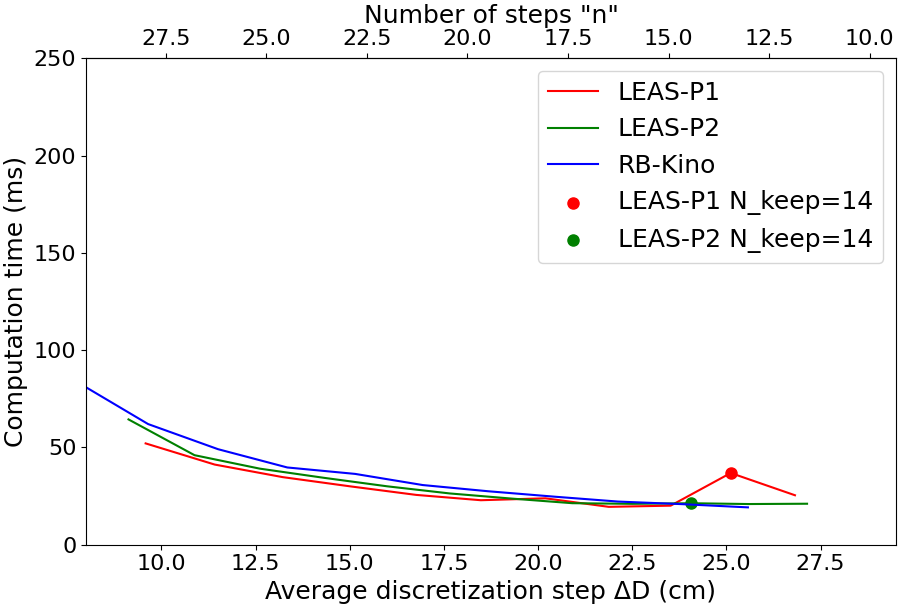
\includegraphics[trim={0cm 0cm 0cm 0cm}, clip,width=\textwidth, height=4cm]{Figures/Chapter_MIP_SL1M/res_mip/time_stairs.png}
    \caption{stairs (up)}
    \label{fig:mip:minimizing_basic:time:0}
    \end{subfigure}
    \begin{subfigure}[t]{0.32\linewidth}
    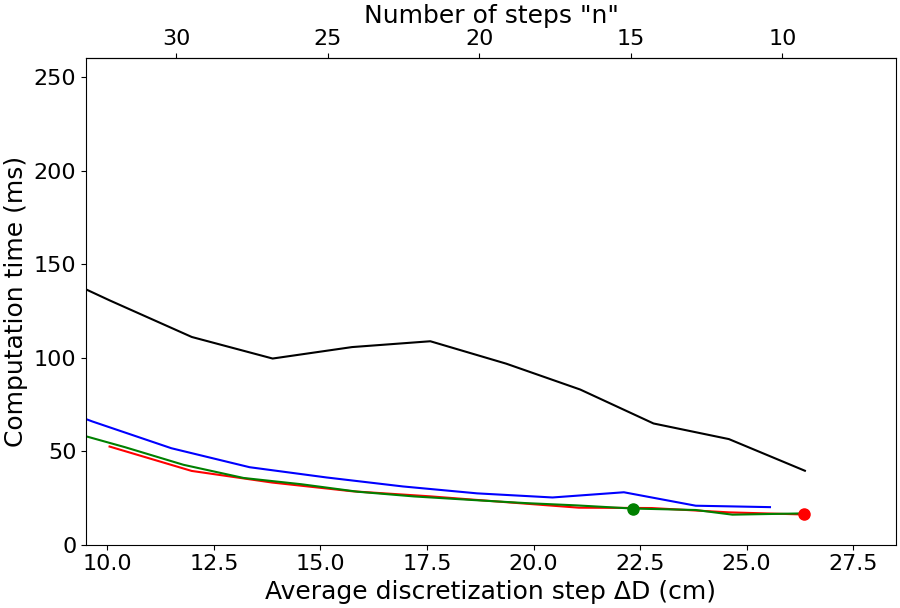
\includegraphics[trim={0cm 0cm 0cm 0cm}, clip,width=\textwidth, height=4cm]{Figures/Chapter_MIP_SL1M/res_mip/time_stairs_down.png}
    \caption{stairs (down)}
    \label{fig:mip:minimizing_basic:time:1}
    \end{subfigure}
    \begin{subfigure}[t]{0.32\linewidth}
    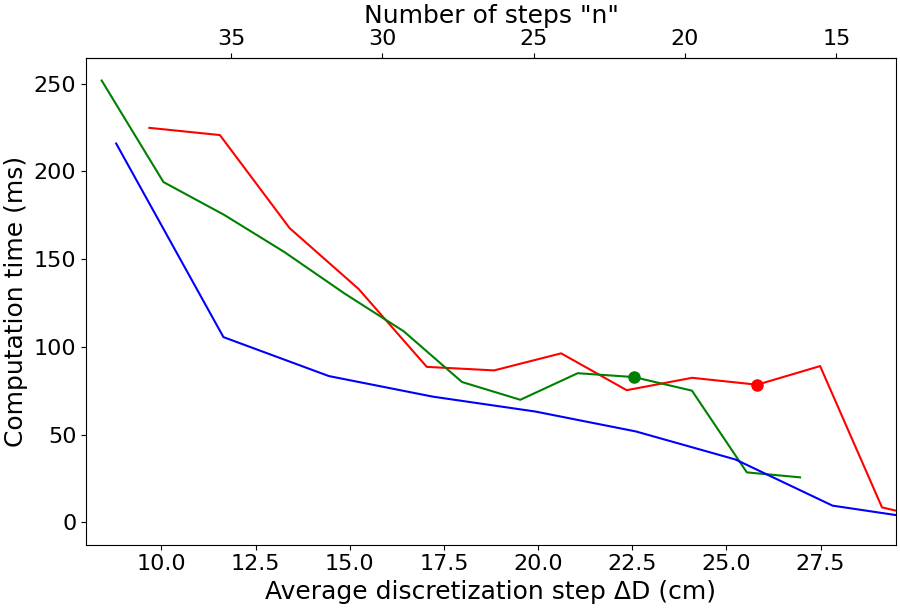
\includegraphics[trim={0cm 0cm 0cm 0cm}, clip,width=\textwidth, height=4cm]{Figures/Chapter_MIP_SL1M/res_mip/time_rubbles.png}
    \caption{rubbles}
    \label{fig:mip:minimizing_basic:time:2}
    \end{subfigure}
    \caption{Contact planning time on guide paths of different average discretization steps. Stairs (a) and (b) contains few surfaces, contrary to the rubbles (c).}
    \label{fig:mip:minimizing_basic:time}
\end{figure}

While a small $\Delta \overline{D}$ increases the contact planning success, it also increases its computation time (Figure \ref{fig:mip:minimizing_basic:time}). As previously discussed, the computation grows exponentially with the number of steps $n$ and their number of candidate surfaces as we can observe on the rubbles.
On contrary, the contact planning time remains relatively low on our stairs scenarios for the tested discretization step range (less than $100$ ms). 
As we can expect, LEAS-P2 for $N_{ref}$ always exhibits an average discretization step with a low computation time, while being successful with the MIP contact planner.


\paragraph{Long scenario.}
% == Success rate and number of footsteps analysis on rubbles ==
% On the big rubble scene => Take 100 traj from anywhere. Use RB-LIN to check the discretization step.
% Plot success rate in function of average delta D => RB-Lin + LEAS-P1 + LEAS-DS
% Plot number of footsteps (states along the guide) for all 4 SM.
% Score = success_rate / nb_footsteps
\begin{figure}[ht]
    \captionsetup[subfigure]{justification=centering}
    \centering
    \begin{subfigure}[t]{0.9\linewidth}
        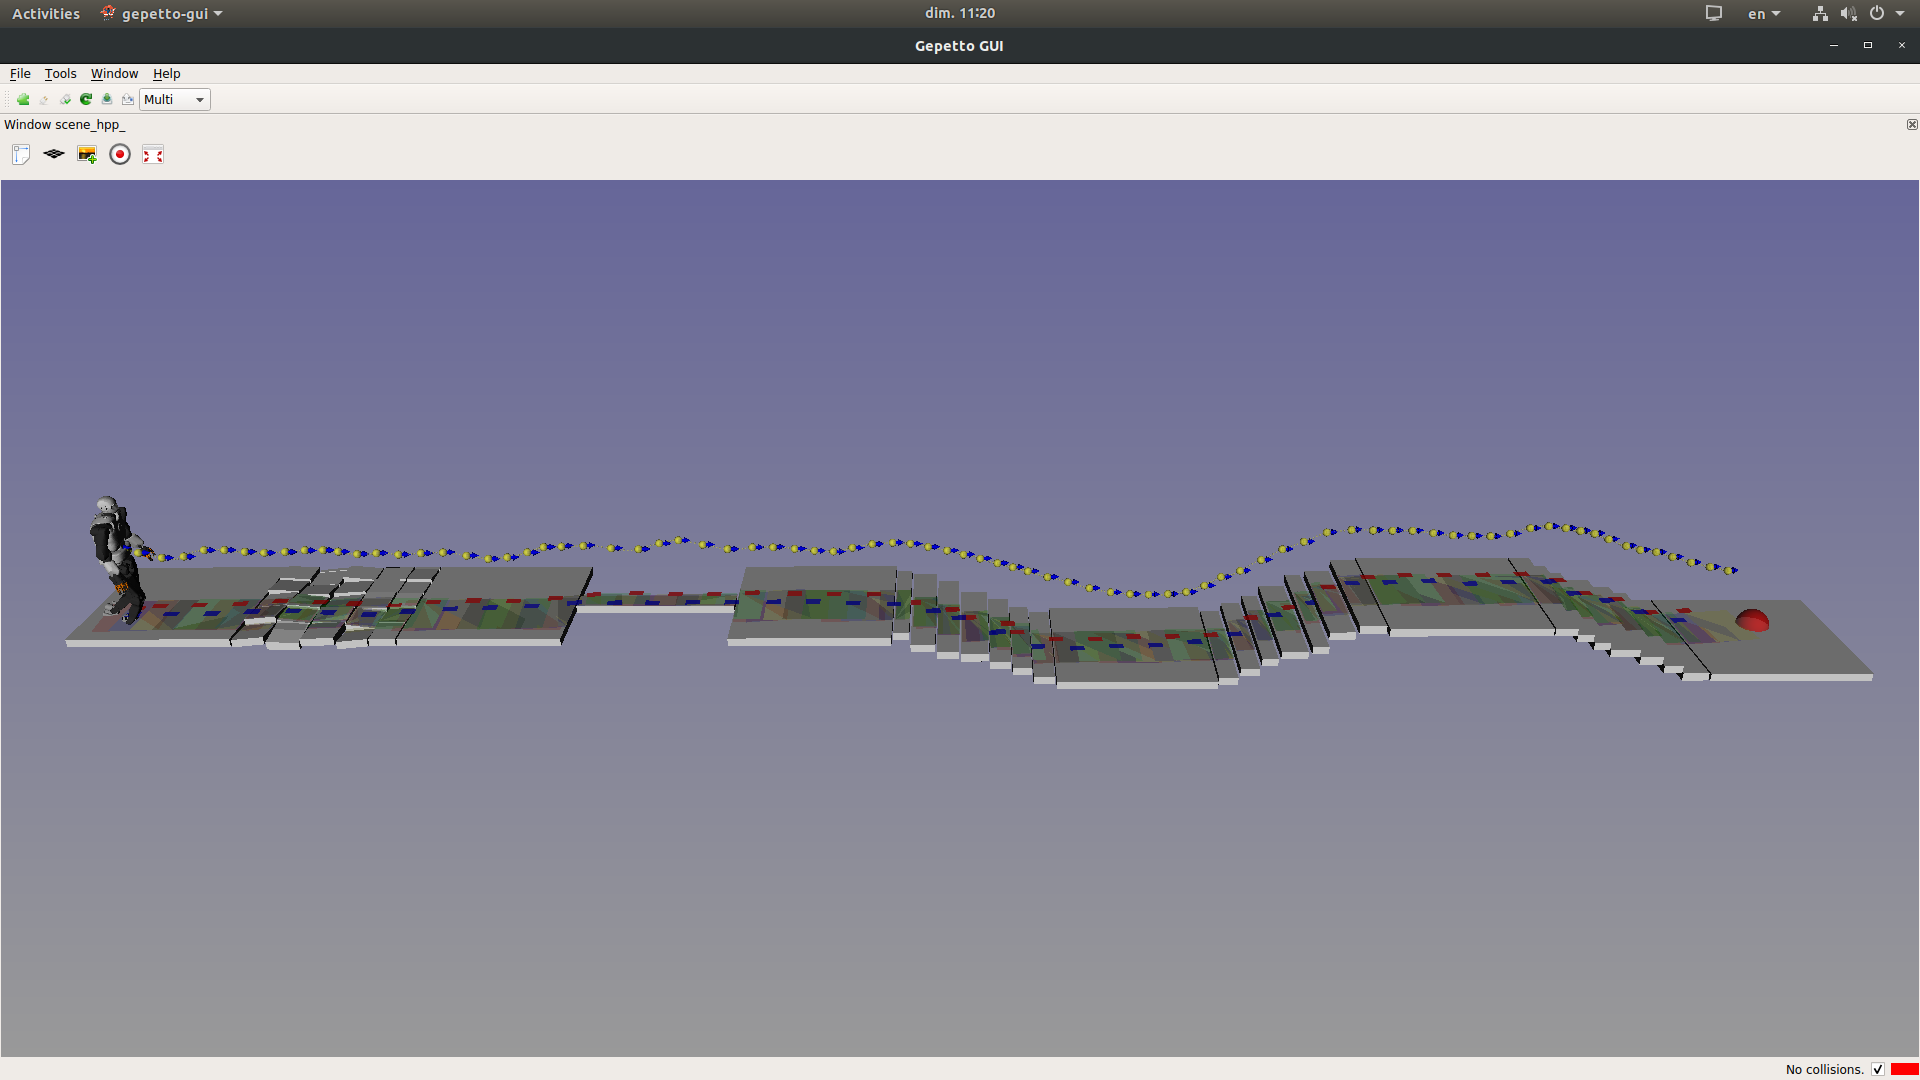
\includegraphics[trim={1cm 12cm 1cm 15cm}, clip,width=\textwidth]{Figures/Chapter_MIP_SL1M/1x11_guide_all_surf_steps.png}
    \end{subfigure}
    \begin{subfigure}[t]{0.9\linewidth}
        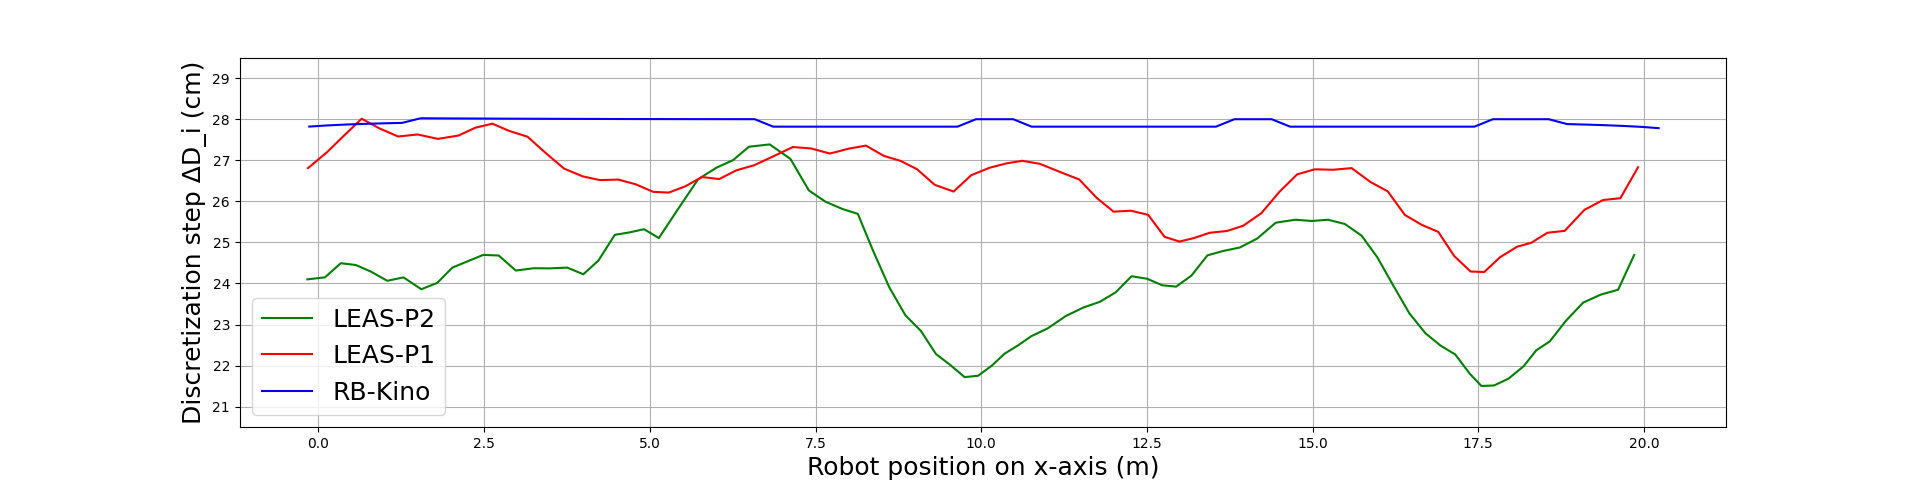
\includegraphics[trim={4cm 0cm 3.5cm 1.5cm}, clip,width=\textwidth]{Figures/Chapter_MIP_SL1M/res_mip/long_discr_x.png}
    \end{subfigure}
    \caption{Example on our long scenario. For each steering method, we plot the discretization steps along the guide path for $N_{ref}$. The x-axis matches the terrain pictured above. The $\Delta D$ value of LEAS-P2 correlates with the terrain difficulty.}
    \label{fig:mip:long_range}
\end{figure}

\begin{figure}[t]
    \centering
    \captionsetup[subfigure]{justification=centering}
    \begin{subfigure}[t]{0.48\linewidth}
    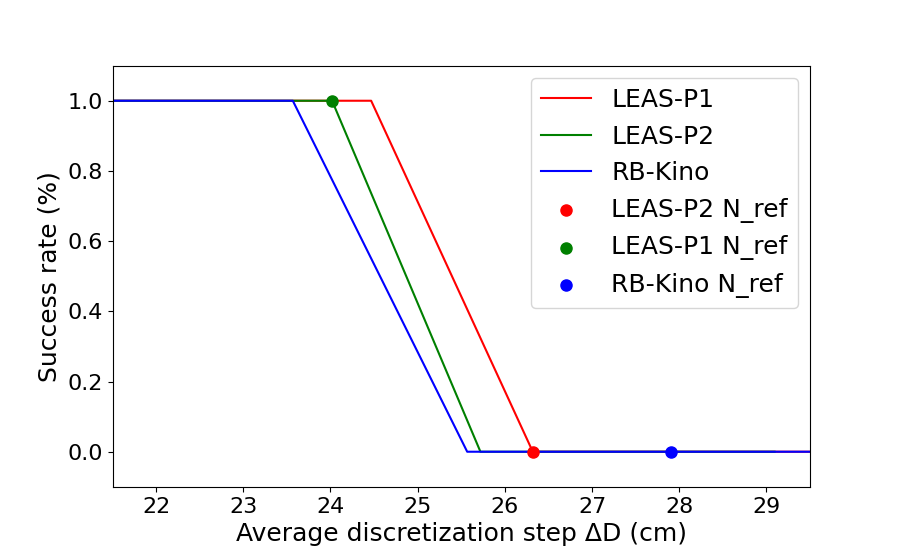
\includegraphics[trim={0cm 0cm 1.9cm 1.6cm}, clip,width=\textwidth, height=4cm]{Figures/Chapter_MIP_SL1M/res_mip/MIP_res_long/FIGURE_MIP_LONG_2.png}
    \caption{}
    \label{fig:mip:long_range_success_time:success}
    \end{subfigure}
    \begin{subfigure}[t]{0.48\linewidth}
    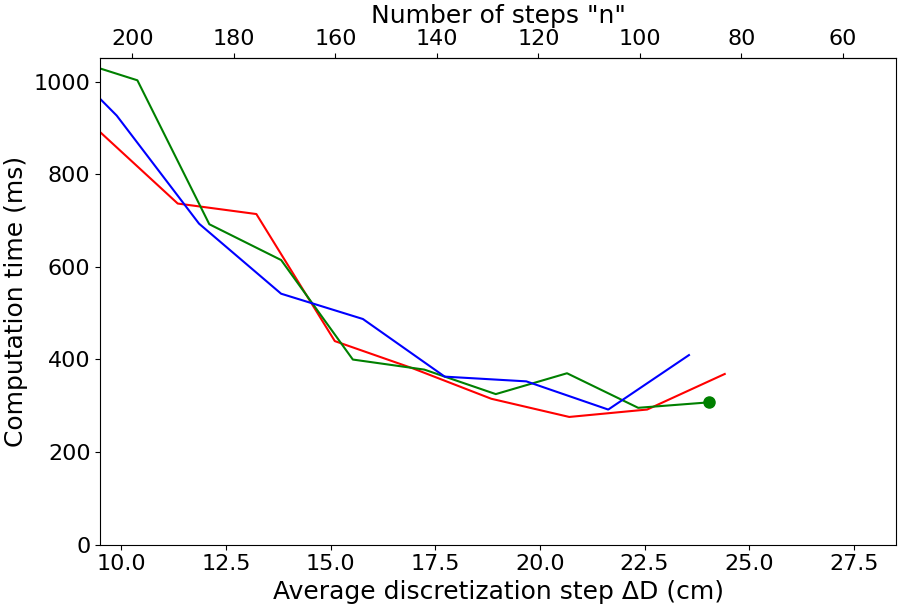
\includegraphics[trim={0cm 0cm 0cm 0cm}, clip,width=\textwidth, height=4.5cm]{Figures/Chapter_MIP_SL1M/res_mip/time_long.png}
    \caption{}
    \label{fig:mip:long_range_success_time:time}
    \end{subfigure}
    \caption{Long scenario for different discretization steps, MIP contact planning (a) success rate and (b) computation time on guide paths of different average discretization steps.}
    \label{fig:mip:long_range_success_time}
\end{figure}

We compare the steering methods on our long-range scenario (Figure \ref{fig:mip:long_range}).
Here, we will further focus on the impact of adapting the discretization $\Delta D_i$ value between each step on a sequence of easy and difficult terrains.

The steering methods have to generate a guide path up to the red objective, then succeed the MIP contact planning.
As RB-Kino can not generate valid guide paths up to the goal without a path planner, we manually place waypoints on the terrain.
This scenario is particularly difficult because the steering method should adapt the discretization step depending on the terrain difficulty.
In that regard, we render the different $\Delta D_i$ values between each step along the guide for $N_{ref}$.
The x-axis matches the terrain pictured so that we can observe the behavior of the steering methods in each terrain area.

We tuned RB-Kino to have an average discretization step of $\Delta \overline{D} \approx 28$ cm along the guide.
Just like in the basic scenarios, LEAS-P1 presents an average discretization step $\Delta \overline{D} \approx 26$ cm.
As both steering methods do not plan guides in function of the terrain difficulty, they both fail the contact planning on our long-range scenario for $N_{ref}$ (Figure \ref{fig:mip:long_range_success_time:success}).

Our solution LEAS-P2 adapts the discretization step for each terrain traversed (Figure \ref{fig:mip:long_range}), which correlates with the results of the basic scenarios. 
We can observe that it exhibits smaller discretization steps on terrains it deemed difficult (rubbles and stairs down), and higher ones on the others (bridge, stairs up, and ground floor).
Thanks to its adaptability, LEAS-P2 can succeed in the MIP contact planning for $N_{ref}$ in our long scenario (Figure \ref{fig:mip:long_range_success_time:success}), whereas other methods require further fine-tuning of the guide discretization.

Finally, we can observe that the MIP contact planner with guide path can compute more than a hundred footsteps at once in relatively short time when the number of steps is optimized (Figure \ref{fig:mip:long_range_success_time:time}).
Just like in the basic scenarios, LEAS-P2 can generate feasible guide paths with the contact planner while exhibiting a sufficiently high discretization between each step. Hence, it permits a tolerable contact planning time, relative to the number of steps planned and the terrain traversed.

\subsection{Conclusion and Discussion}
\label{subsub:mip:discussion}
\paragraph{Conclusion.}
We explained the formulation for contact planning with a continuous approach using Mixed-Integer Programming.
Then we explained the benefits of using a guide path in this formulation, as done in the previous work \cite{sl1m_v2}.
The main limitation of their approach was the required fine-tuning of the guide discretization.

To solve this limitation, we presented a solution using our steering method LEAS to automatically generate a guide path with a suitable discretization step along it, depending on the terrain difficulty.
As a result, it can generate feasible problems for the MIP contact planner while reducing the number of steps, hence the overall contact planning time.

%\textcolor{blue}{En vrai tous les scenarios que j'ai presente sont faisable avec une discretisation moyenne de 20-22cm, pour des temps de calcul similaire. Comment je peux tourner ca en quelque chose de plus positifs? On me posera forcement des questions dessus.}


\paragraph{Traversability estimation.}
As discussed in Chapter \cite{sec:LEAS}, tuning the upper and lower bounds of the z-value in the height map is critical to have a correct terrain representation.
Trivially, setting wider bounds will permit better detection of large obstacles, or differentiate stairs and void. However, it hinders the detection of small height variations on the terrain such as rubbles.
Several strategies could be explored to fix such problems, such as using convolutional neural networks as previously discussed, or giving as observation a second tighter bounded height map.

In this thesis, we keep the height map bounds used in previous chapters and we add to the number of potential candidate surfaces around the robot as an observable state.
This state permits LEAS to better detect difficult terrains, however, it is still unclear how this parameter impacts the agent decision and additional ablation tests are required.
In the future, other methods could be explored to estimate the terrain traversability \cite{lin_traversability_2018, brandao_multimode_2019}.
%was required as values in the observable height map were not accurate enough to efficiently detect small height variations on scenarios like rubbles.

\paragraph{Contact planning awareness and guide discretization.}
We discretize the guide path in the input of the contact planner by keeping 1 out of $N_{ref}$ configurations.
However, our RL agent does not know which state corresponds to a step inside the contact planner.
As a consequence, our steering method only adapts the robot velocity along the guide depending on the terrain, and implicitly the discretization steps $\Delta D$.
In another experiment, we added another observable scalar representing a counter before the next step to be performed as well as the distance and local height map from the previous step. However, it did not improve LEAS results.

Another option is for LEAS to output directly the next root configuration $q$ from which a contact is to be made.
This approach can remove the need to filter the guide path ($N=1$).
Hence, this control could potentially permit the agent to directly control the discretization step and to accurately select suitable candidate surfaces $\mathcal{S}_i$.
In our experiments, we implemented such an approach by raising the timestep $T$ and controlling LEAS in velocity (instead of acceleration). 
However as discussed in Chapter \ref{sec:CP-SB}, it was not achievable in practice regarding the learning stability, because of the large actions the RL agent does.

\paragraph{Pruning candidates surfaces.\label{subsub:mip:discussion:candidate_surfaces}}
%\begin{figure}[t]
%    \centering
%    \captionsetup[subfigure]{justification=centering}
%    \begin{subfigure}[t]{0.48\linewidth}
%    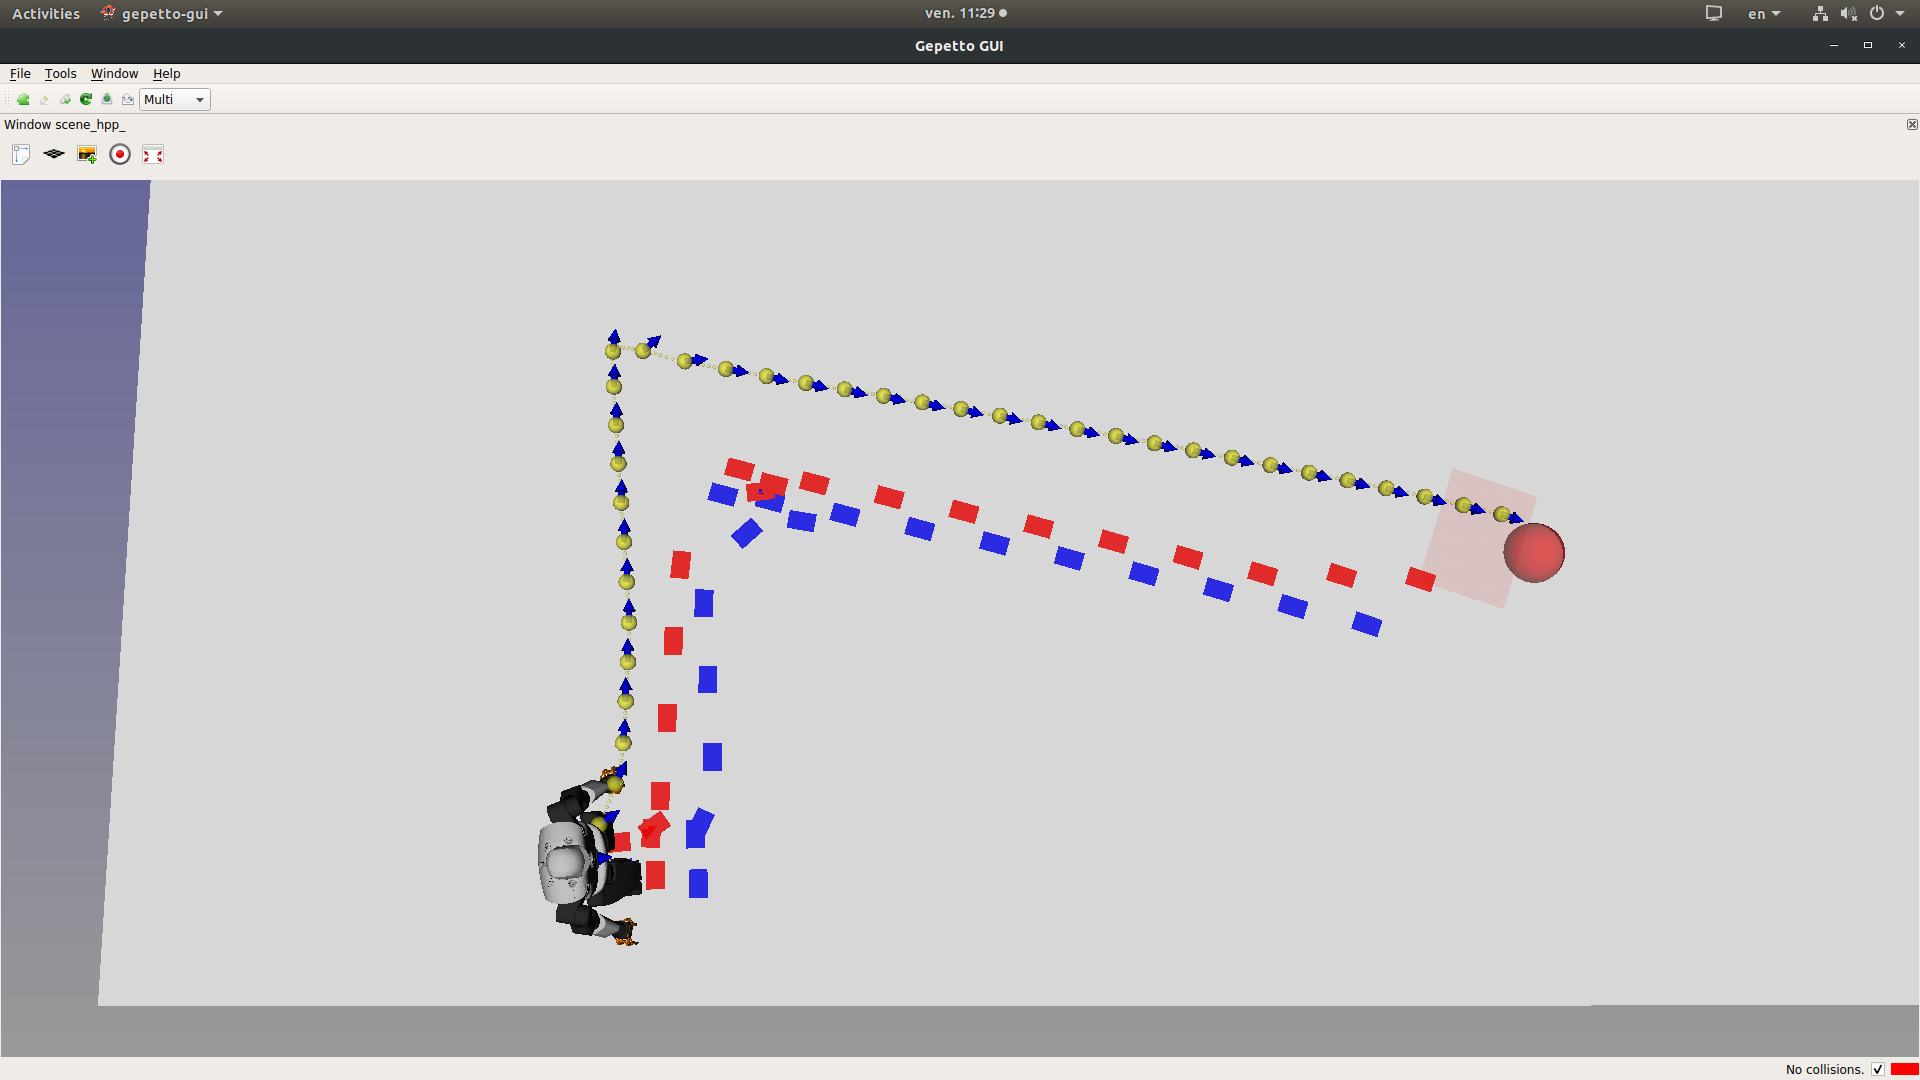
\includegraphics[trim={15cm 4cm 10cm 9cm},clip,width=\textwidth,height=4cm]{Figures/Chapter_MIP_SL1M/flat_candidate_surf/ground_guide_uncontrained.png}
%    \caption{}
%    \label{fig:mip:flat:unconstrained}
%    \end{subfigure}
%    \begin{subfigure}[t]{0.48\linewidth}
%    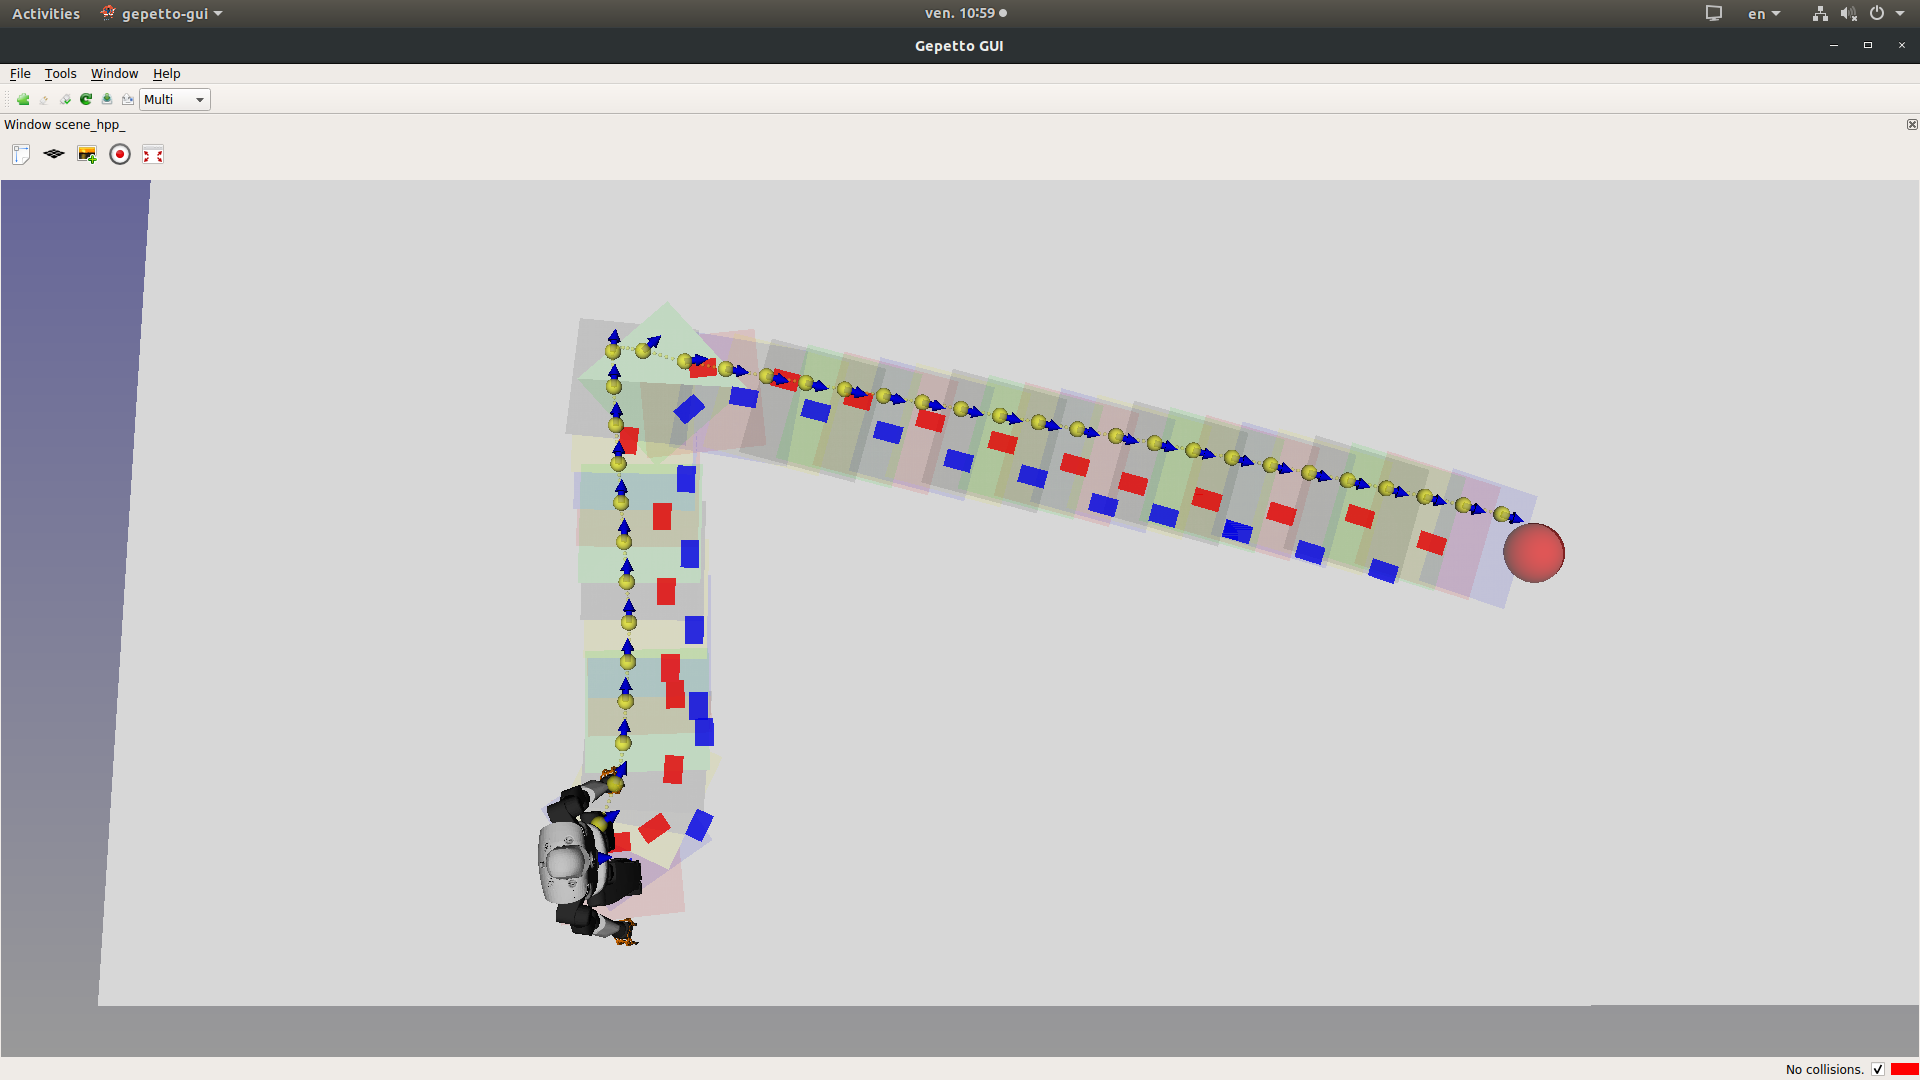
\includegraphics[trim={15cm 4cm 10cm 9cm},clip,width=\textwidth,height=4cm]{Figures/Chapter_MIP_SL1M/flat_candidate_surf/ground_guide_contrained.png}
%    \caption{}
%    \label{fig:mip:flat:constrained}
%    \end{subfigure}
%    \caption{Contact planning along the guide: (a) on the whole flat surface $\mathcal{S}^{flat}$, and (b) around the guide on the colored surface intersections $\mathcal{S}_i \in \mathcal{S}^{flat}$.}
%    \label{fig:mip:flat:constrained_or_not}
%\end{figure}
% La HM est petite 80x80. C'etait necessaire pour contraindre la recherche de pas autour. Autrement 
In this thesis, we obtain the candidate surfaces for each step from a height map centered around the robot root configuration. While the height map size could be enlarged to offer more possibilities and thus increase the problem feasibility.
We choose such a small size to constrain the search for contacts only in the guide path vicinity.

Other strategies are available to obtain the candidate surfaces $\mathcal{S}_i$.
In the previous work \cite{sl1m_v2}, Song et al. use the range of motion of the robot legs (See constraint $\mathcal{C}$ in Chapter \ref{sec:LEAS}).
If an intersection exists between this range of motion at $\mbox{q}_i$ and a surface $\mathcal{S}^j$, then the entire surface is added to the set $\mathcal{S}_i$.
Adding the complete reachable surfaces $\mathcal{S}^j$ sure increases the feasibility of the problem. 
However, it may not constrain enough the search for footsteps around the guide, which can be a limitation depending on the locomotion task.


\paragraph{Reinforcement learning and combinatorics.}
% Does the RL really solves a combinatorics problem here ? No real control on the problem.
% He just say the number of steps in the end...

We emphasize the fact that the MIP contact planner solves the discrete choice of contact surfaces, which is a combinatorial problem.
%Indeed, the problems we presented are solved along all the trajectory at once, as opposed to a short horizon planning approach \cite{fanny_mip_solo}.
Our steering method adapts the robot velocity along the guide path depending on the terrain, that then composes the problem to solve. 
However, LEAS can not observe the past trajectory. 
As a consequence, it is not directly (or not at all) aware of its combinatorial aspect. 

As discussed in the previous work \cite{sl1m_v2}, pruning surfaces along the guide can be seen as a MIP presolve routine (cuts) specific to contact planning.
This strategy often leads to small feasibility problems to be solved with only a few to no exploration of the combinatorics when using a presolver \cite{presolve_gurobi_2020}.
However, this is not the case for more complex scenarios in which contact planning time increases due to the computation of the branch-and-bound algorithm that handles the combinatorial aspect of the problem (i.e. selection of surfaces).

While we demonstrate the efficacy of this approach with Gurobi solver \cite{gurobi}, the contact planning time highly depends on the MIP solver used, as well as its various methods and heuristics employed.
Moreover, state-of-the-art MIP solvers can be quite large in terms of memory size which limits their embedding on real robots.
An interesting problem thus naturally arises: \textit{Can we reformulate the problem as a simple linear program and remove the need to explore the combinatorics?}

%However, it may not be the same when adding a quadratic cost $l(\mbox{P},\mbox{R})$ to the problem. 
%Further exploring other methods, more specifically with machine learning, to accelerate the solving of these problems is an exciting direction \cite{deepmind_RL_MIP}.

%\textcolor{red}{Steve: La transition ici marche pas, il faut parler de l'exploration des noeuds. Et ensuite dire on pense que du coup, on peut se passer du framewok MIP qui est lourd et ptet formuler juste un LP si on arrive a virer la combi, et la transitioner sur SL1M.}
%\textcolor{blue}{Fixed. J'ai essaye d'introduire au mieux SL1M dans le section d'apres, ca suffit?}

% =================================================


\section{Reformulation of a Feasibility Problem: SL1M}
\label{sub:mip:sl1m}
%We presented in previous section a Mixed-Integer Programming formulation for contact planning.
%This problem is solved by a classical branch-and-bound algorithm to solve its combinatorics \cite{gurobi_mip}.

%However, commercial MIP solvers can not easily be embedded on robots due to their memory size and computation power required.
This section investigates an answer to the question: can we solve the MIP contact planning without the need for a branch-and-bound algorithm?
As a result, it could be solved using a simple linear solver.
%The continuous contact planning approach presented is inherently subject to the combinatorics of the surfaces selection. As a consequence, reformulating it as a linear problem is not trivial. 
It is the objective of the reformulation called SL1M \cite{sl1m_v1} presented in this section.

\subsection{Relaxation of the Mixed-Integer Problem}
% Show the reformulation with a guide path => Constraint stated above.
% Reformulation into a feasibility problem => Minimize l1-norm inside the MIP (no quadratic cost) + surfaces never intersect + remove the constraint on nb of surfaces.
% How does gurobi solve it? => In fact the first step is SL1M?
% Two ways: use a MIP for a branch&bound, or use only some LP but lose the guarantee of completeness.
% Put the results here for relaxation.
In the previous work \cite{sl1m_v1}, a relaxation of the MIP formulation for contact planning is proposed.
The relaxed formulation using a guide path is as follows:
\begin{align}
    \textrm{\textbf{given}} %\quad & \mathcal{I}=\{p_0^{left}, \mbox{r}_0^{left},p_0^{right}, \mbox{r}_0^{right}\} \nonumber\\
    %\textrm{, the initial foot position}\\
                            %\quad & n\\%\textrm{, the desired number of contacts}\\
                            %\quad & \mathcal{S}=\{\mathcal{S}^0,...,\mathcal{S}^m\}\\%\textrm{, the set of terrain surfaces}\\
                            %\quad & \mathcal{S}^{goal}\\%\textrm{, the goal surface to reach}\\
                            \quad & n, \;\mbox{p}_0, \; \mbox{r}_0, \; \mathcal{S}^{goal} \nonumber\\
                            \quad & R=[\mbox{r}_1,...,\mbox{r}_n], \; \mbox{r}_i \in \mathbb{R}^{3} \nonumber\\
                            \quad & C=[\mathcal{S}_0, ..., \mathcal{S}_n] \nonumber\\
    \textrm{\textbf{find}}  \quad & \mbox{P}=[\mbox{p}_1,...,\mbox{p}_n], \;\mbox{p}_i \in \mathbb{R}^{3} \nonumber\\
                            \quad & \textcolor{blue}{\alpha=[\alpha_1,...,\alpha_n], \; \alpha_i \in \mathbb{R}_{+}^{m_i}} \label{eq:mbc:sl1m:slack_relaxed}\\
                            \quad & \beta=[\beta_1,...,\beta_n], \; \beta_i \in \mathbb{R}^{m_i} \nonumber\\
                            %\quad & \alpha=[\alpha_1,...,\alpha_n] \in \mathbb{R}_{+}^{n}\\
    \textrm{\textbf{min}}  \quad & \textcolor{blue}{\sum_{i=1}^{n} \sum_{j=1}^{m_i} \alpha_i^j} \label{eq:mbc:sl1m:norm_l1}\\
    \textrm{\textbf{s.t.}}  \quad & \{\mbox{P},\mbox{R}\} \in \mathcal{I} \cap \mathcal{G} \cap \mathcal{F} \nonumber\\
                            \quad & \forall i \in \{1,..,n\} : \nonumber\\
                                \quad & \quad \forall j \in \{1,..,m_i\} : \nonumber\\
                                    \quad & \quad \quad S_i^j\mbox{p}_i \leq s_i^j + M \textcolor{blue}{\alpha_i^j} \textbf{1} \nonumber\\
                                    \quad & \quad \quad (\mbox{p}_i)^{\intercal} \textbf{n}^j = e^j + \beta_i^j \nonumber\\
                                    \quad & \quad \quad ||\beta_i^j||_1 \leq M \textcolor{blue}{\alpha_i^j} \nonumber\\
                                    \nonumber
\end{align}
\paragraph{Reformulation.}
Contrary to the MIP formulation, the integrality constraint on the slack variables is relaxed (\ref{eq:mbc:sl1m:slack_relaxed}). 
As a result, the problem can be solved with a linear or quadratic solver.

The most important change is the reformulation of the feasibility problem into a cardinality minimization problem. The cardinality constraint of the MIP formulation is replaced by a $l1$-norm minimization (\ref{eq:mbc:sl1m:norm_l1}).
Indeed, $l1$-norm minimization has long been used in optimization problems to induce sparsity (i.e. encourage the convergence of the slack variables to 0) \cite{boyd2004convex}. 
In this formulation for contact planning, having an $\alpha_i^j$ with a 0 value means that the candidate surface $\mathcal{S}_i^j$ has been selected for the $i$-th footstep. 
As a result, the $l1$-norm encourages the selection of surfaces for each step.
In the next Section \ref{subsub:insight_l1}, we will provide further insight on the $l1$-norm to visually understand how it encourages this sparsity in the contact planning context.

%However, this formulation also implies that for each step $i$, all surfaces in $\mathcal{S}_i$ must be disjoint:
%\begin{equation}
%    \forall i \in \{1,...,n\},\; \cap^m_{j=1} \mathcal{S}^j_i = 0
%\end{equation}
%In other words, it is impossible for a footstep to lie on two surfaces at the same time. This condition is required, otherwise the foot position $\mbox{p}_i$ will automatically lie at the intersection between these surfaces to miminize the $l1$-norm.


\paragraph{Solution to the relaxed problem.\label{par:sl1m:solution_relaxed_heuristics}}
The problem is directly solved if exactly one surface is selected for each footstep:
\begin{equation}
    \label{eq:sl1m:pb_solved}
    \forall i \in \{1,...,n\},\; \exists! j \in \{1,...,m\},\; \alpha^j_i = 0
\end{equation}
If the problem is not solved after this relaxation, as is usually the case, several strategies are available to enforce this condition.

As previously discussed, a branch-and-bound approach can efficiently solve this problem. 
However, it requires the use of a heavy MIP solver.

Another approach is to explore the combinatorics with heuristics.
In \cite{sl1m_v2}, Song et al. fix all the slack variables $\alpha_i$ for which the cardinality constraint is satisfied (i.e. $\alpha_i=0$). 
They then test all the combinations for the remaining free variables until either i) a solution is found, ii) a maximum number of trials is reached, or iii) all possibilities are exhausted. 
%\stn{je comprends pas ça} \textcolor{blue}{Fixed. Est-ce que j'ai le droit de copier la strategie du papier sl1m mot à mot?}

\subsection{Insight on the Relaxation}
\label{subsub:insight_l1}
% Now I focus on the first step, the relaxation of the integer variables.
% I will show the gradient in function of surfaces + cost in function of foot position + relation between the different groups (phases)
% Can we further improve it with LEAS?
To better understand how the $l1$-norm encourages surface selection, we propose several scenarios with a visual understanding of SL1M solutions.

\paragraph{Big-M method and $l1$-norm without constraints.}
\begin{figure}[ht]
    \centering
    \captionsetup[subfigure]{justification=centering}
    \begin{subfigure}[t]{0.48\linewidth}
    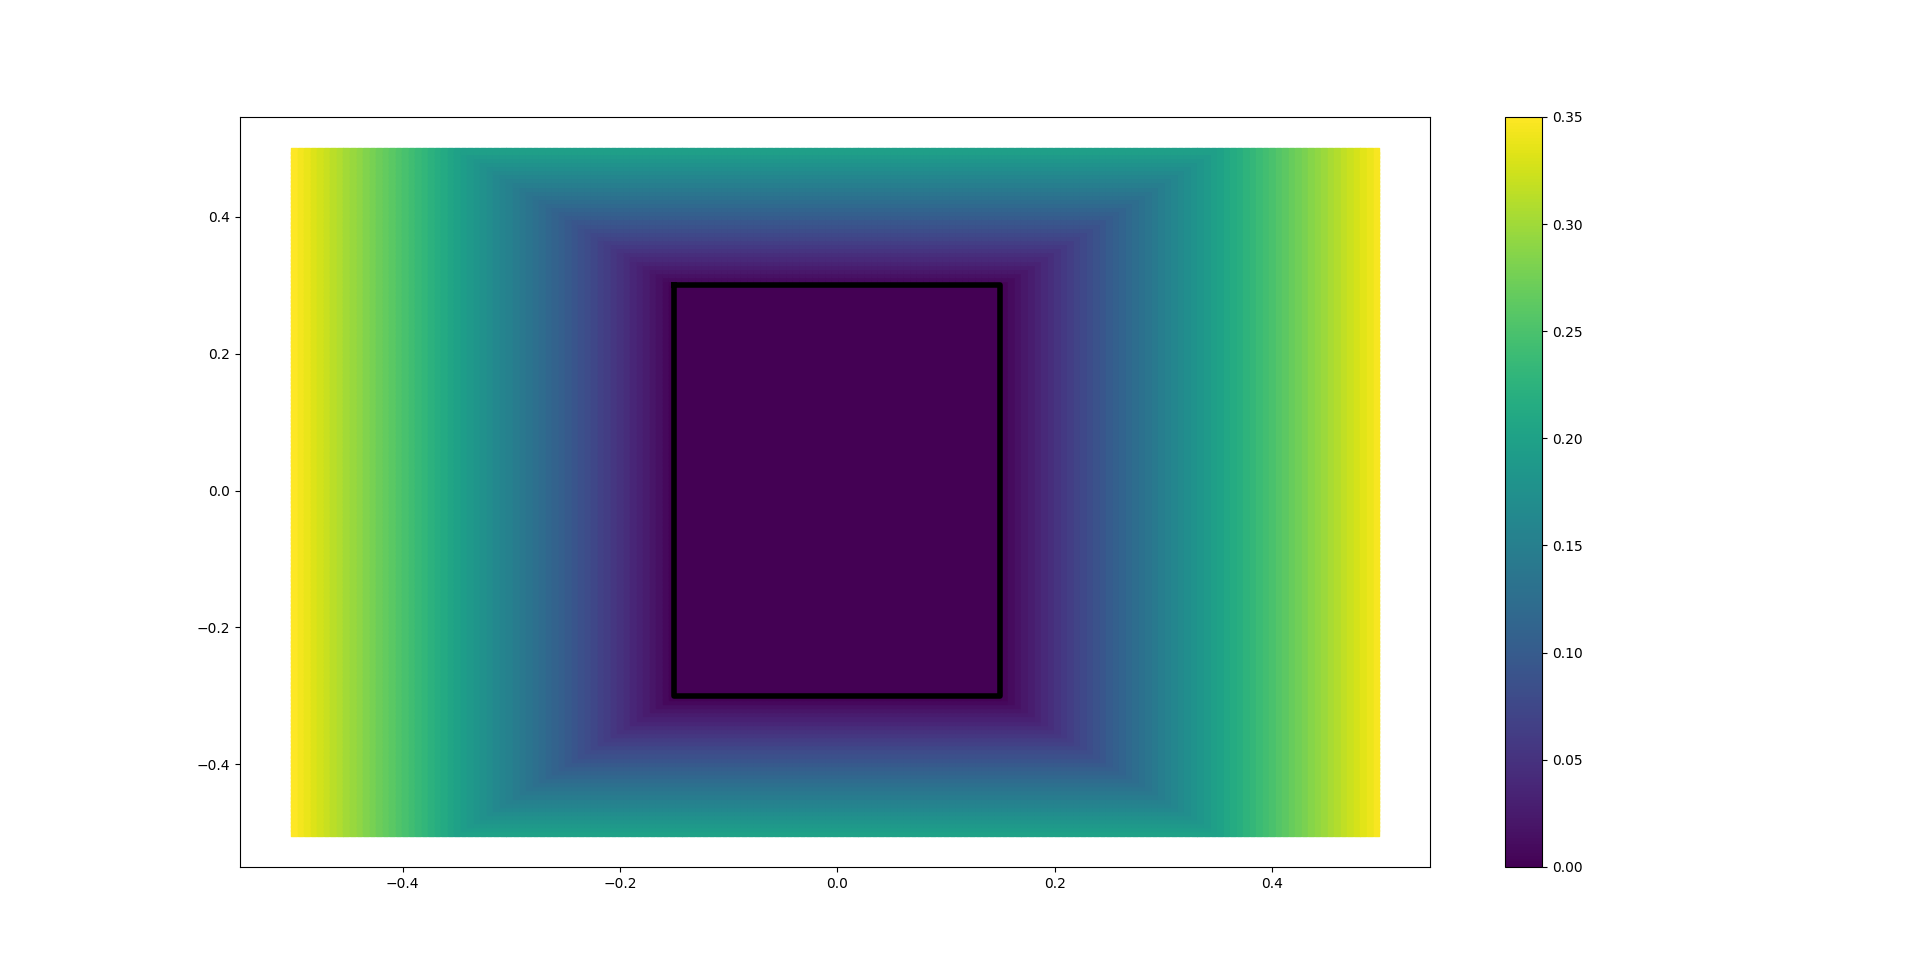
\includegraphics[trim={5cm 2cm 12cm 2cm},clip,width=\textwidth]{Figures/Chapter_MIP_SL1M/l1_no_cst/grad_simple_0.png}
    %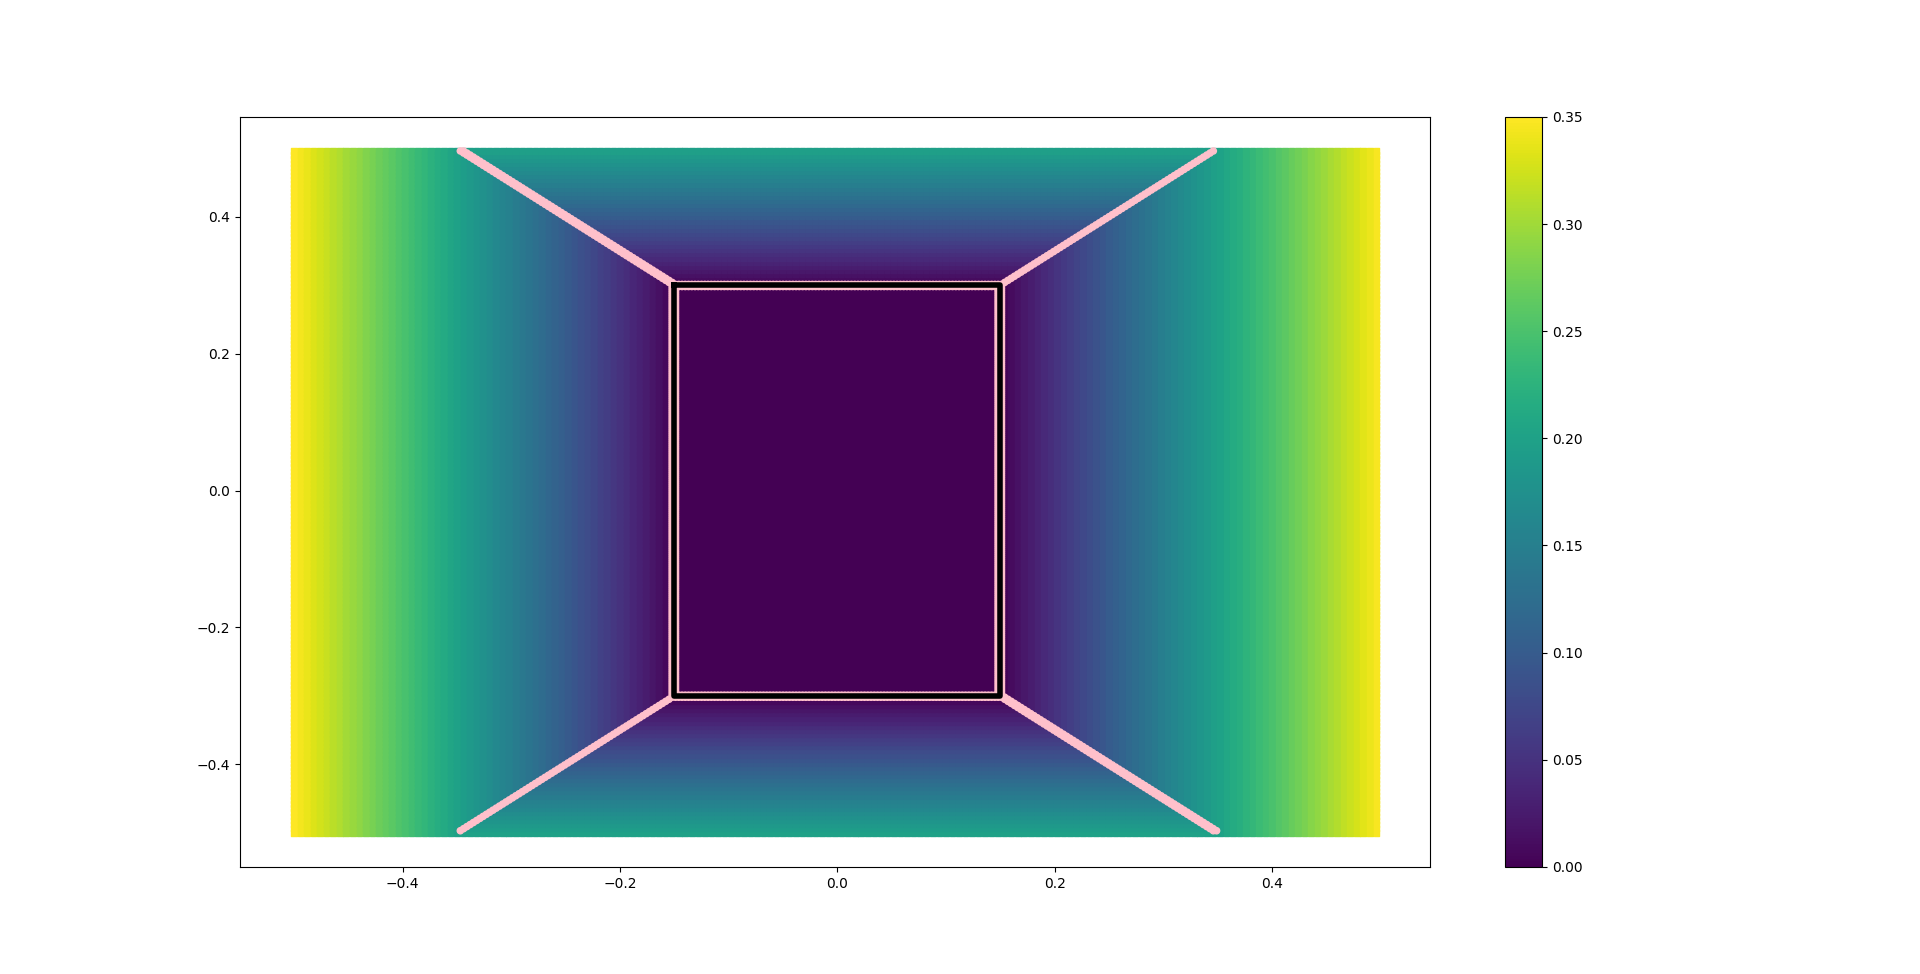
\includegraphics[trim={0 0 12cm 0},clip,width=\textwidth]{Figures/Chapter_MIP_SL1M/l1_no_cst/grad_simple_0_limit.png}
    %\caption{}
    \end{subfigure}
    \begin{subfigure}[t]{0.48\linewidth}
    %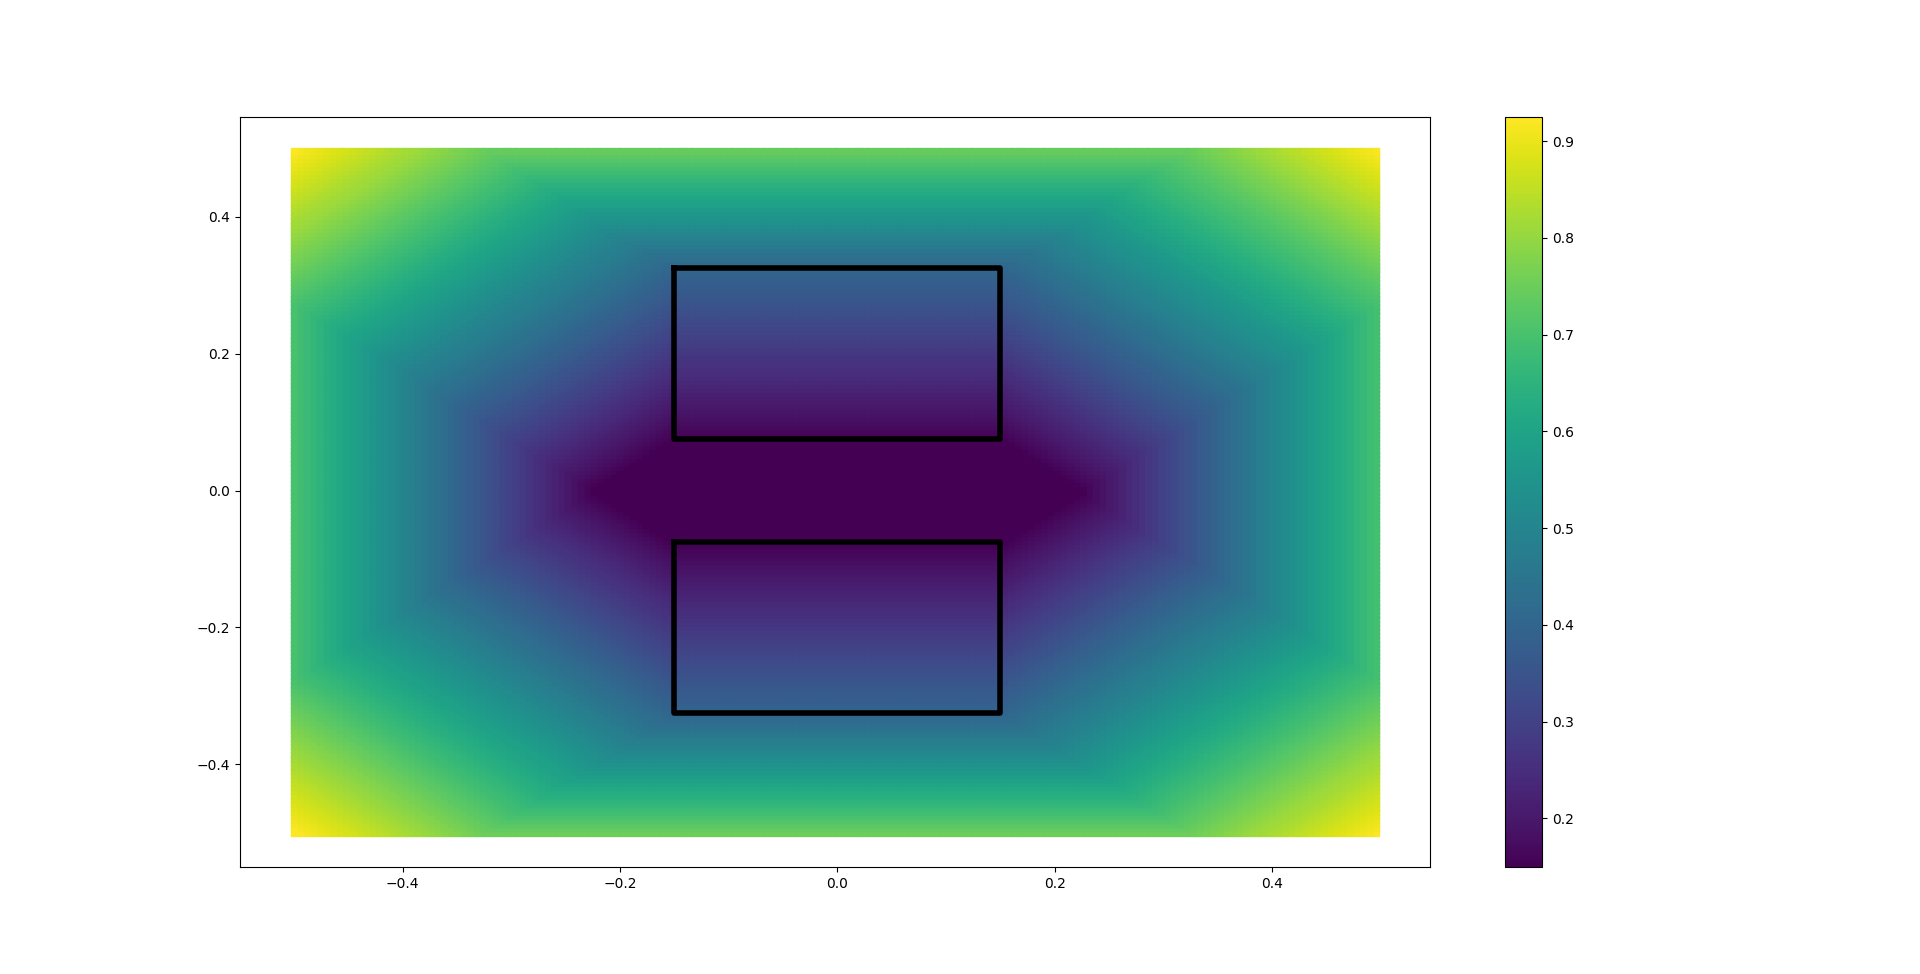
\includegraphics[trim={5cm 2cm 12cm 2cm},clip,width=\textwidth]{Figures/Chapter_MIP_SL1M/l1_no_cst/grad_two_0_1.png}
    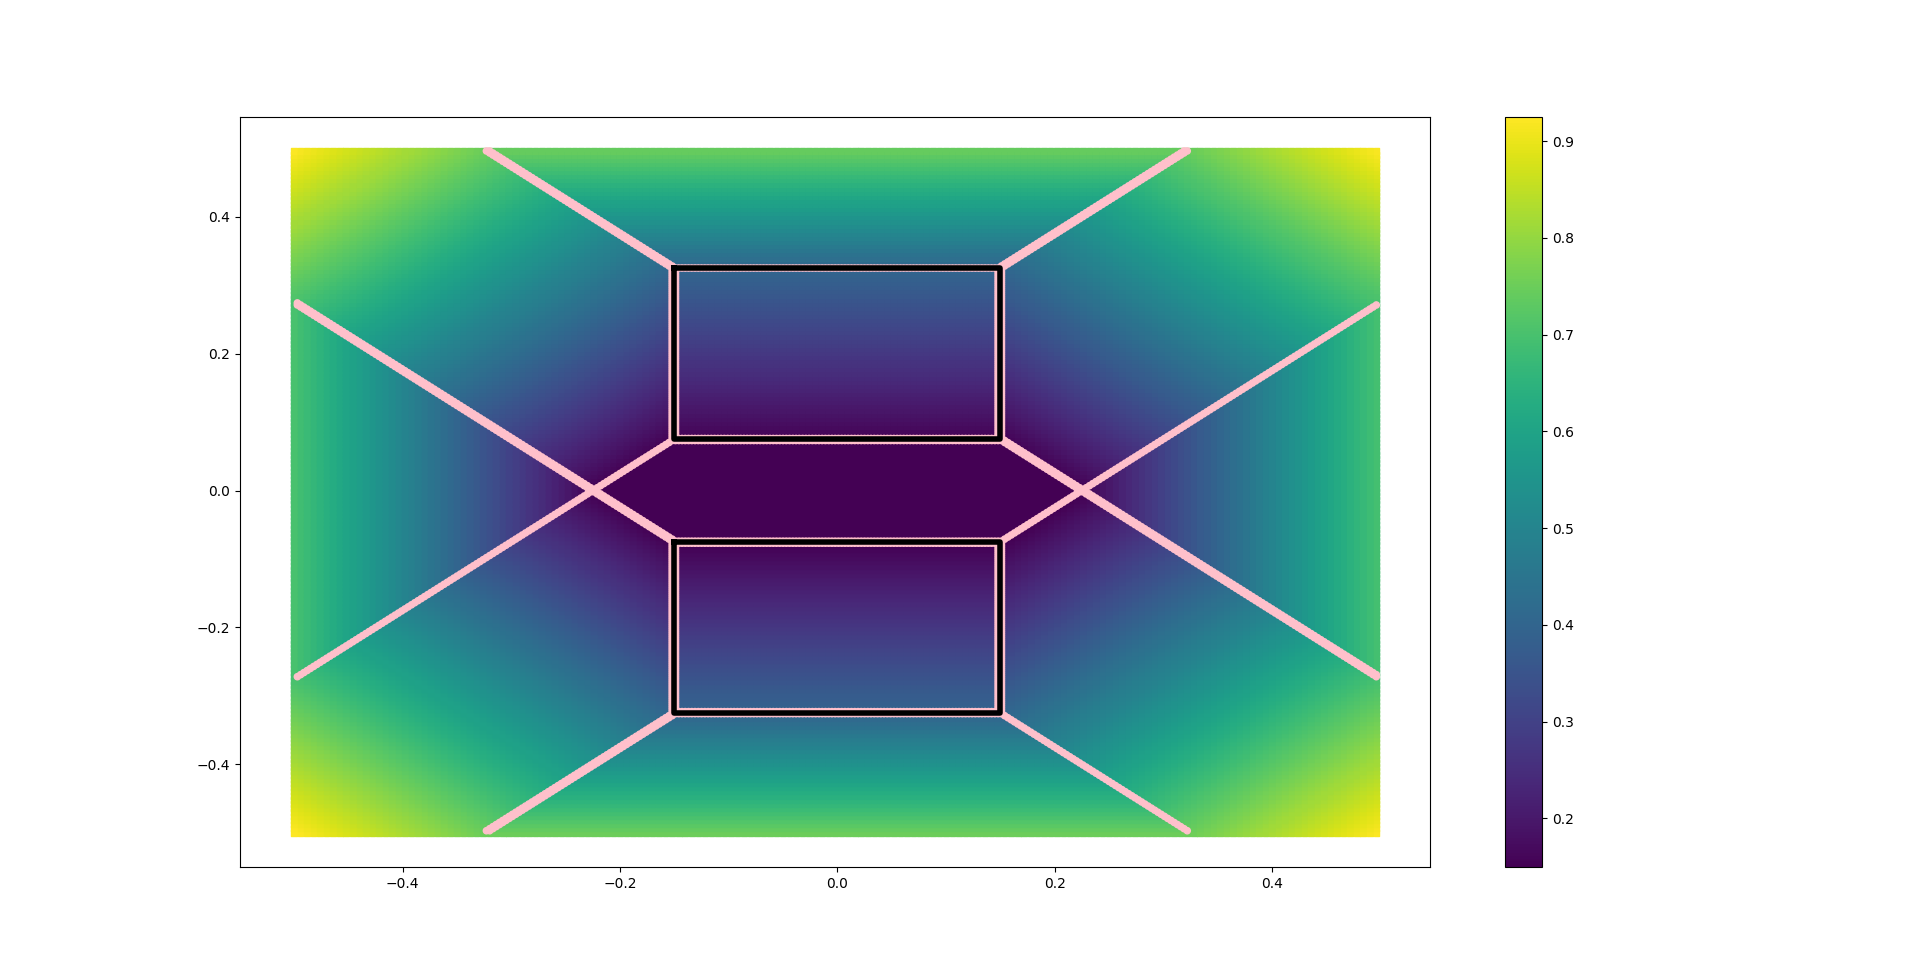
\includegraphics[trim={5cm 2cm 12cm 2cm},clip,width=\textwidth]{Figures/Chapter_MIP_SL1M/l1_no_cst/grad_two_0_1_limit.png}
    %\begin{tikzpicture}
    %    \draw (0, 0) node[inner sep=0] {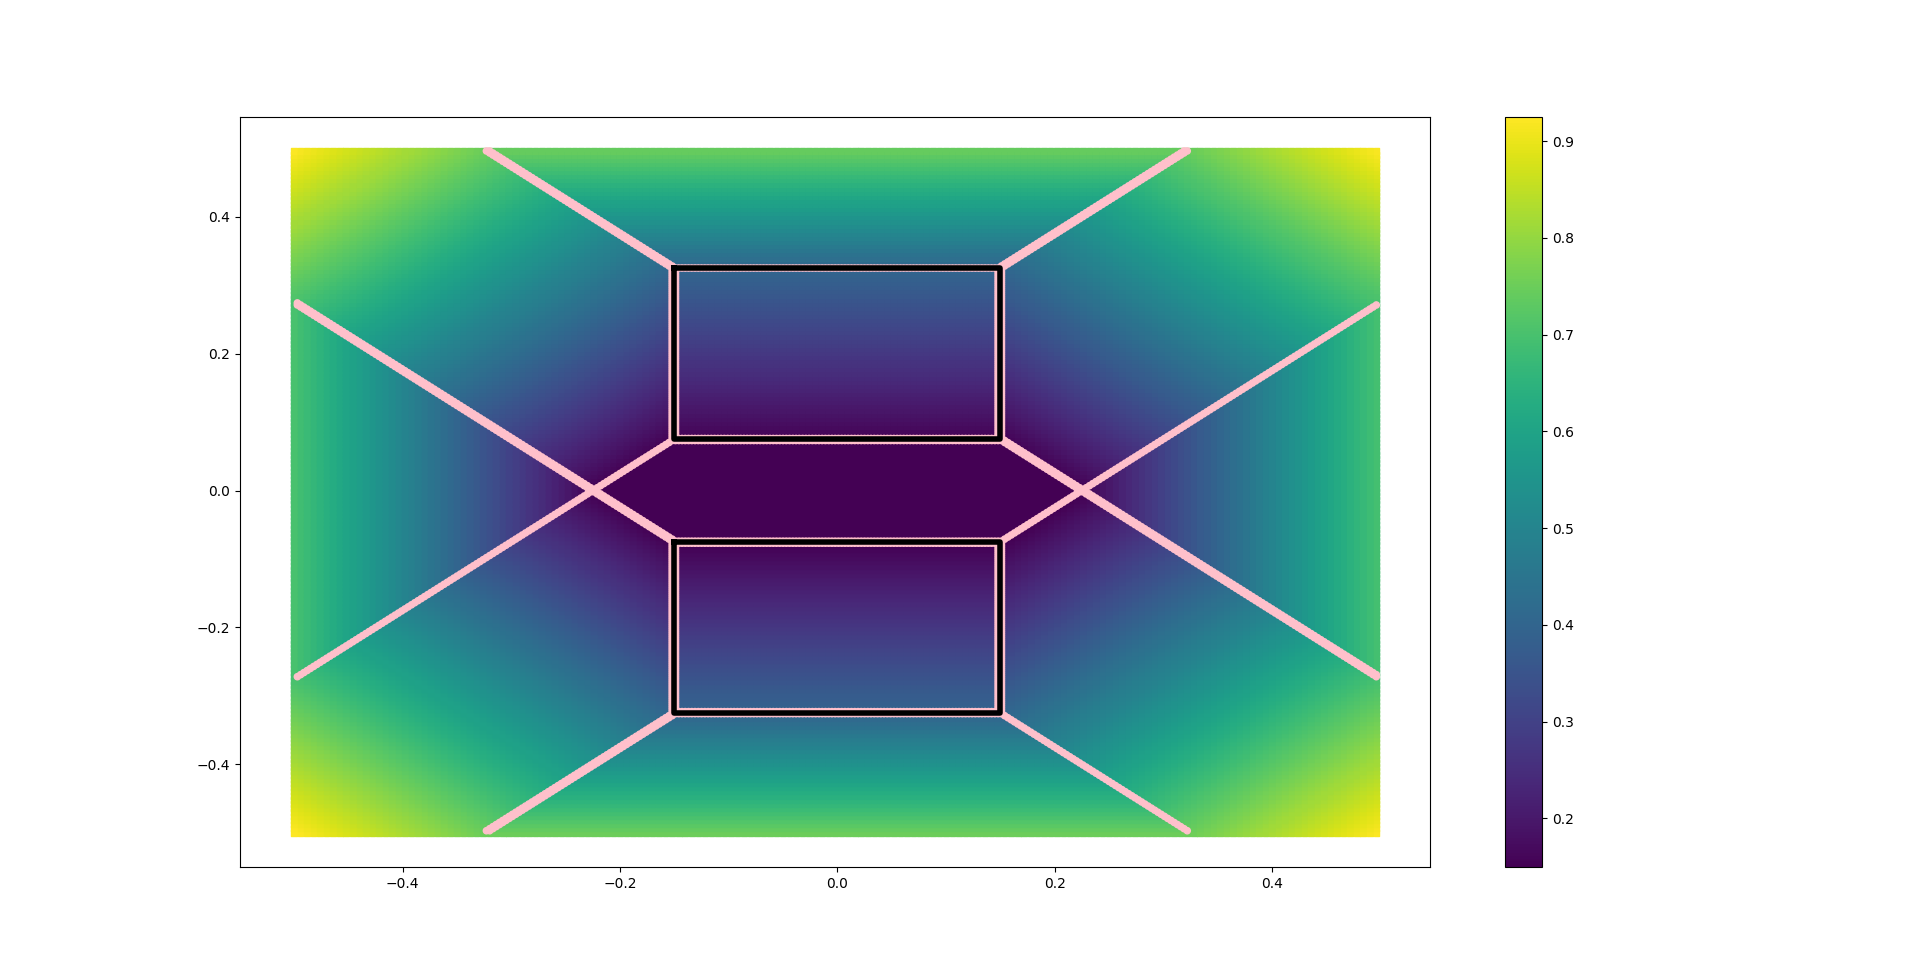
\includegraphics[trim={5cm 2cm 12cm 2cm},clip,width=\textwidth]{Figures/Chapter_MIP_SL1M/l1_no_cst/grad_two_0_1_limit.png}};
        % ARROWS
        % grad 2
        %horizontal
    %    \draw [white,-to](-3,0) -- (-2.5,0);
    %    \draw [white,-to](3.15,0) -- (2.65,0);
    %    \draw [white,-to](0,-2) -- (0,-1.5);
    %    \draw [white,-to](0,1.93) -- (0,1.43);
        %vertical
    %    \draw [white,-to](-3,-2) -- (-2.56,-1.65);
    %    \draw [white,-to](-3,1.93) -- (-2.58,1.65);
    %    \draw [white,-to](3.15,-2) -- (2.71,-1.65);
    %    \draw [white,-to](3.15,1.93) -- (2.73,1.65);
    %\end{tikzpicture}
    %\caption{}
    \end{subfigure}
    \begin{subfigure}[t]{0.48\linewidth}
    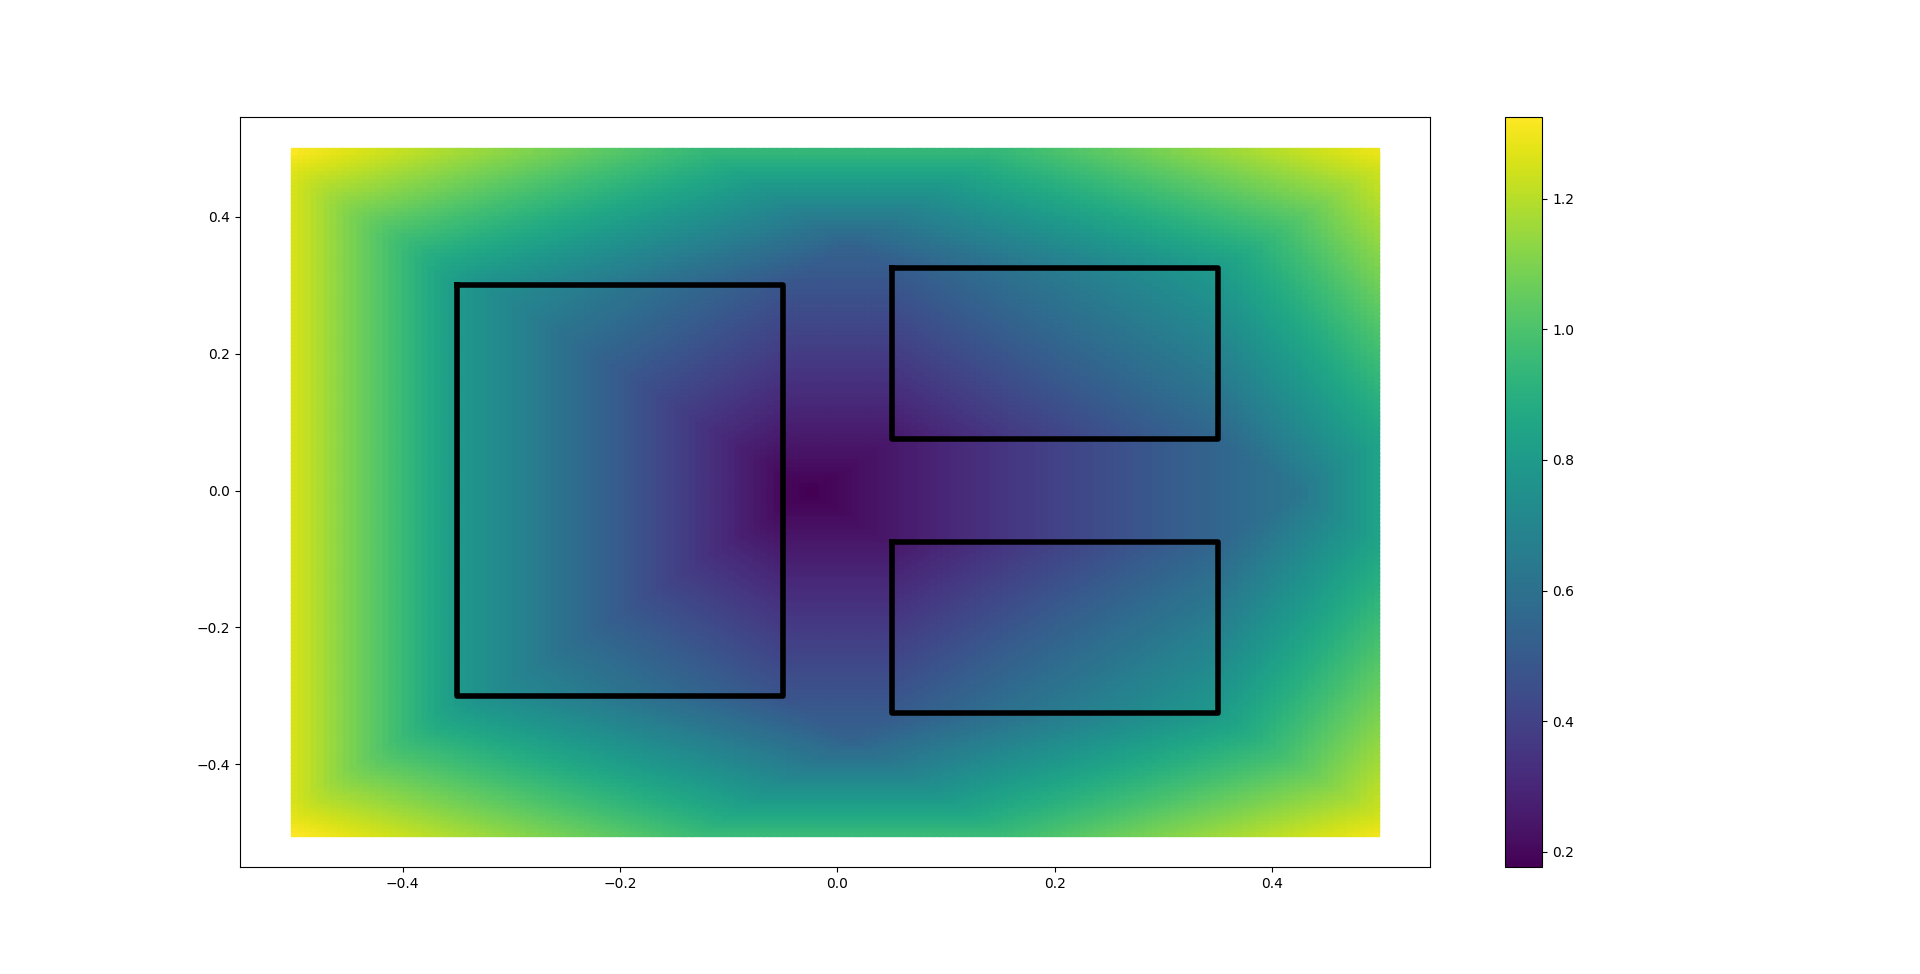
\includegraphics[trim={5cm 2cm 12cm 2cm},clip,width=\textwidth]{Figures/Chapter_MIP_SL1M/l1_no_cst/grad_three_0_1_2.png}
    %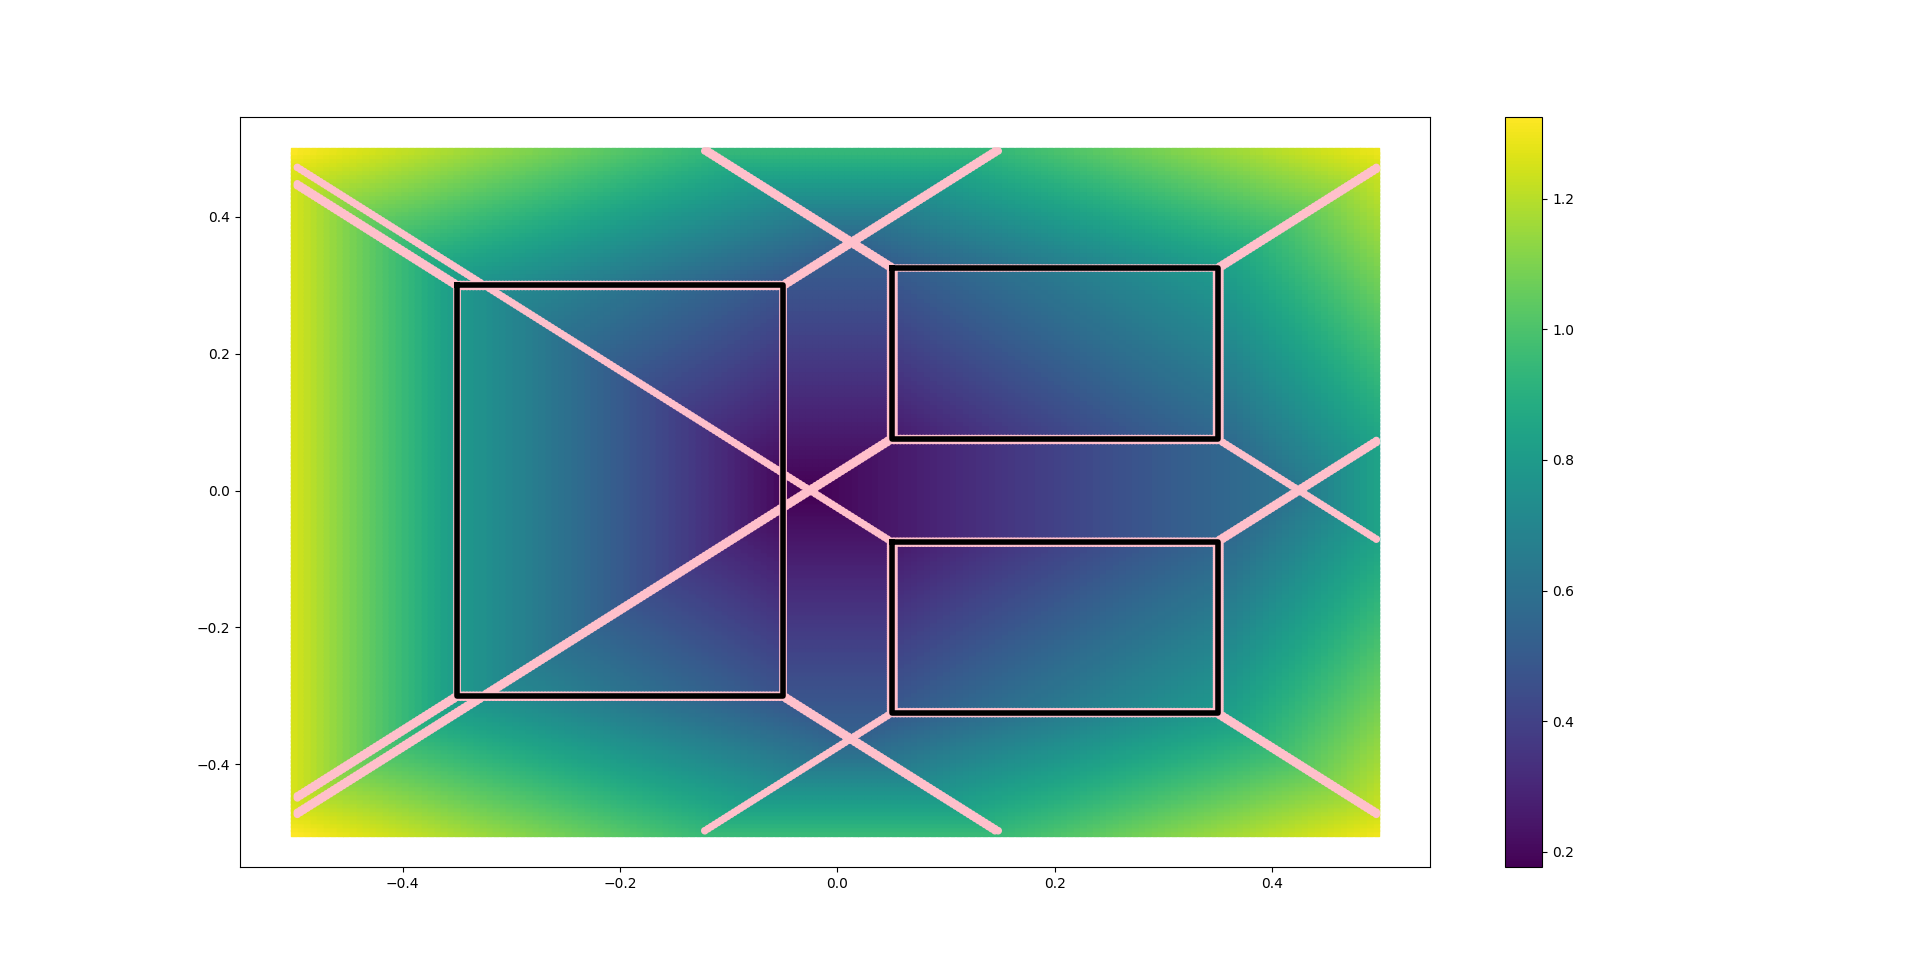
\includegraphics[trim={0 0 12cm 0},clip,width=\textwidth]{Figures/Chapter_MIP_SL1M/l1_no_cst/grad_three_0_1_2_limit.png}
    %\caption{}
    \end{subfigure}
    \begin{subfigure}[t]{0.48\linewidth}
    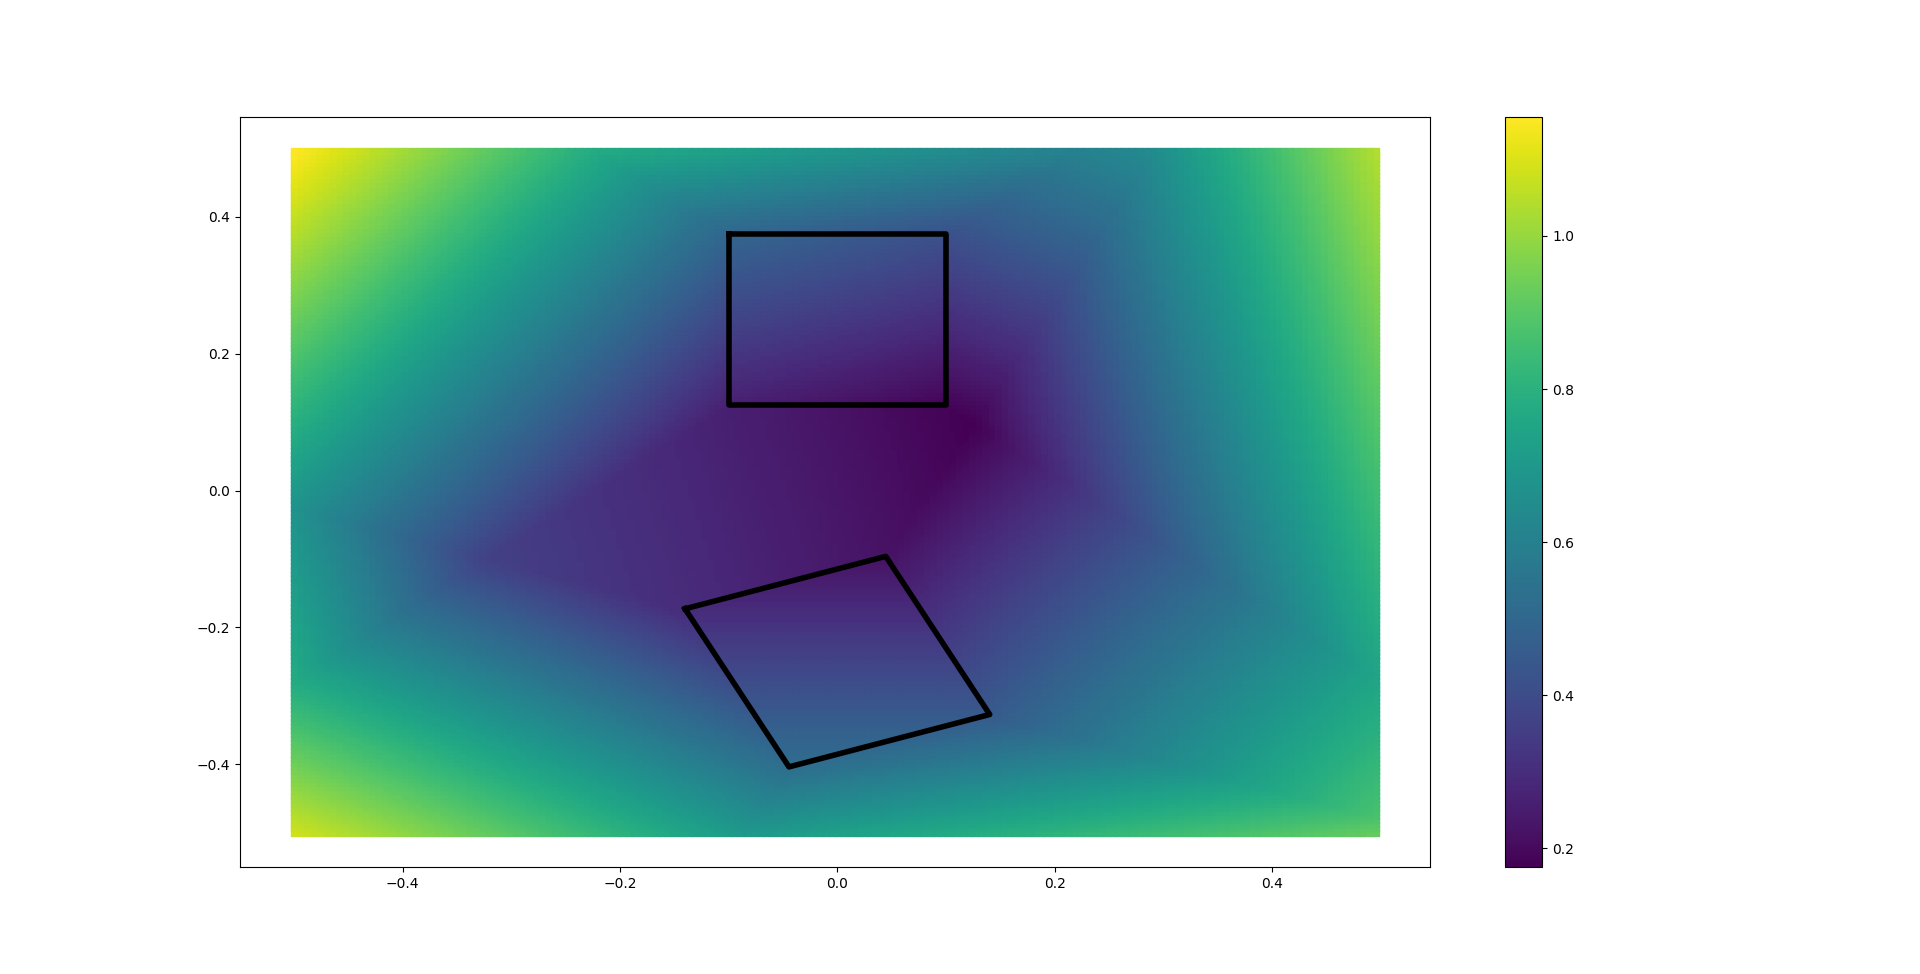
\includegraphics[trim={5cm 2cm 12cm 2cm},clip,width=\textwidth]{Figures/Chapter_MIP_SL1M/l1_no_cst/grad_simple_rotate.png}
    %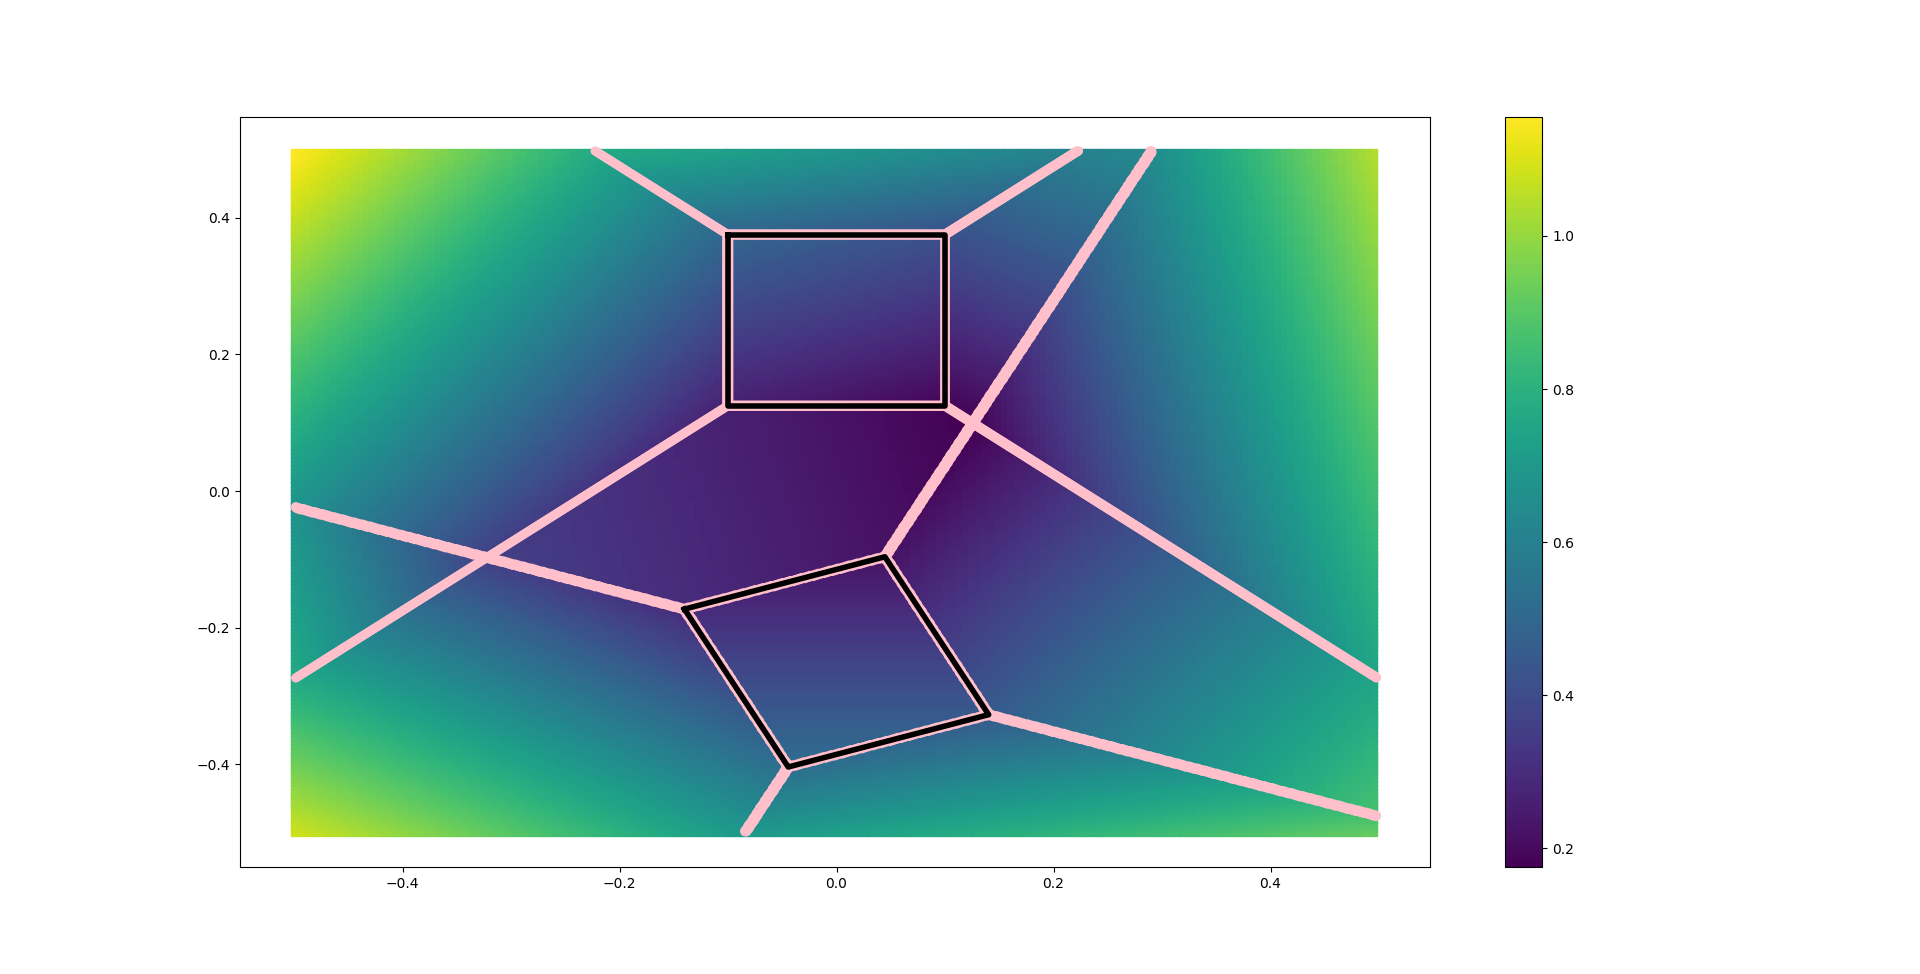
\includegraphics[trim={0 0 12cm 0},clip,width=\textwidth]{Figures/Chapter_MIP_SL1M/l1_no_cst/grad_simple_rotate_limit.png}
    %\caption{}
    \end{subfigure}
    \caption{Example of $l1$-norm cost (\ref{eq:mbc:sl1m:no_constr_l1}) relative to different surfaces sample in 2D: dark shades represent a low cost and bright shades a high cost. The pink lines in the top right figure delimits the gradient changes.}
    \label{fig:sl1m:no_constraint}
\end{figure}
We give the following simplified formulation of our problem:
\begin{align}
    \textrm{\textbf{given}} \quad & \mathcal{S}, \mbox{p} \nonumber\\
    \textrm{\textbf{find}}  \quad & \alpha=[\alpha^1,...,\alpha^m],\; \alpha^j \in \mathbb{R}_{+} \nonumber\\
    \textrm{\textbf{min}}  \quad & \sum_{j=1}^{m_i} \alpha^j \label{eq:mbc:sl1m:no_constr_l1}\\
    \textrm{\textbf{s.t.}}  \quad & \quad \forall j \in \{1,..,m\} : \nonumber\\
                            \quad & \quad \quad S^j \mbox{p} \leq s^j + M \alpha^j \textbf{1} \nonumber\\
                            \nonumber
\end{align}
For each position p in the 2D space, we aim to minimize the $l1$-norm relative to the surfaces $\mathcal{S}^j \subset \mathcal{S}$. 
Results for different surfaces sample are shown in Figure \ref{fig:sl1m:no_constraint}.
Black rectangles represent the terrain surfaces $\mathcal{S}^j$.
We represent the $l1$-norm cost (\ref{eq:mbc:sl1m:no_constr_l1}) on a 2D map, where the gradient changes from bright to dark to represent higher and lower cost value respectively.
In the top right figure, we highlight in pink the delimitation between the different gradient cost areas (i.e. where the gradient of the $l1$-norm changes in strength or direction).
These delimitations show that there always exists a change of gradient on the edges of the surfaces, which already hints at how sparsity is encouraged in SL1M.

In the solution (\ref{eq:mbc:sl1m:no_constr_l1}), each $\alpha^j$ measure the distance between the point position p and the closest edge of surface $\mathcal{S}^j$.
We now want to understand what is the consequence of such a formulation in the context of contact planning.


\paragraph{Scenario A.}
% Show the simple where it works.
% Show the one where it doesn't.

In all following scenarios, we simplify the feasibility constraints $\mathcal{F}$ (See Appendix \ref{appendix:feasibility_constr}).
We will use only the constraints on the foot positions, represented by the red and yellow rectangles in our scenarios (left and right foot respectively).
The rotation r$_i$ is kept constant for all footsteps, so that all constraints are oriented in the same direction.
As a consequence, the foot position p$_i$ is only constrained by the previous foot position p$_{i-1}$.
We do so to have a better visual understanding of SL1M relative to these simple constraints.

In both scenarios (Figures \ref{fig:sl1m:a11} and \ref{fig:sl1m:a12}), the robot from its initial right foot position p$_1$ (yellow dots) has to reach the surface $\mathcal{S}^4$ in two steps. 
To do so, we arbitrarily assign to the step position p$_2$ the candidate surfaces of indices 2 and 3 (i.e. $\mathcal{S}^2$ and $\mathcal{S}^3$).
We plot the $l1$-norm cost map for this step only, as it is the only one given multiple surface candidates.

In scenario A.1 (Figure \ref{fig:sl1m:a11}), the feet positions p$_2$ and p$_3$ computed by SL1M relaxation both lies at the edges of their respective constraints. 
This is expected as we are solving a linear problem using the simplex algorithm, which explores the edges of the feasibility constraints.
Also, the feet position p$_2$ is attracted by the $l1$-norm minimum area between the surface $\mathcal{S}^2$ and $\mathcal{S}^3$. 
In this scenario, the problem is solved after the first relaxation as one surface has been selected for each step.

In scenario A.2 (Figure \ref{fig:sl1m:a12}), the result shows that the foot position p$_2$ still lies at the edge of the foot constraint, and is placed in the minimum $l1$-norm minimum area. 
However, it does not lie on a surface ($\alpha_1^2 > 0$ and $\alpha_1^2 > 0$), and so our problem is not solved.
As discussed in Section \ref{par:sl1m:solution_relaxed_heuristics}, we can use some heuristics to explore the combinatorics. 
The heuristics previously presented generate 2 sub-problems as p$_2$ has 2 candidate surfaces.
The first combination tested is $p_2 \in \mathcal{S}^2$, its closest surface.
In this scenario, the heuristics is successful with the first combination (Figure \ref{fig:sl1m:a12:1}).

\begin{figure}[ht]
    \centering
    \captionsetup[subfigure]{justification=centering}
    \begin{subfigure}[t]{0.48\linewidth}
    \begin{tikzpicture}
        \draw (0, 0) node[inner sep=0] {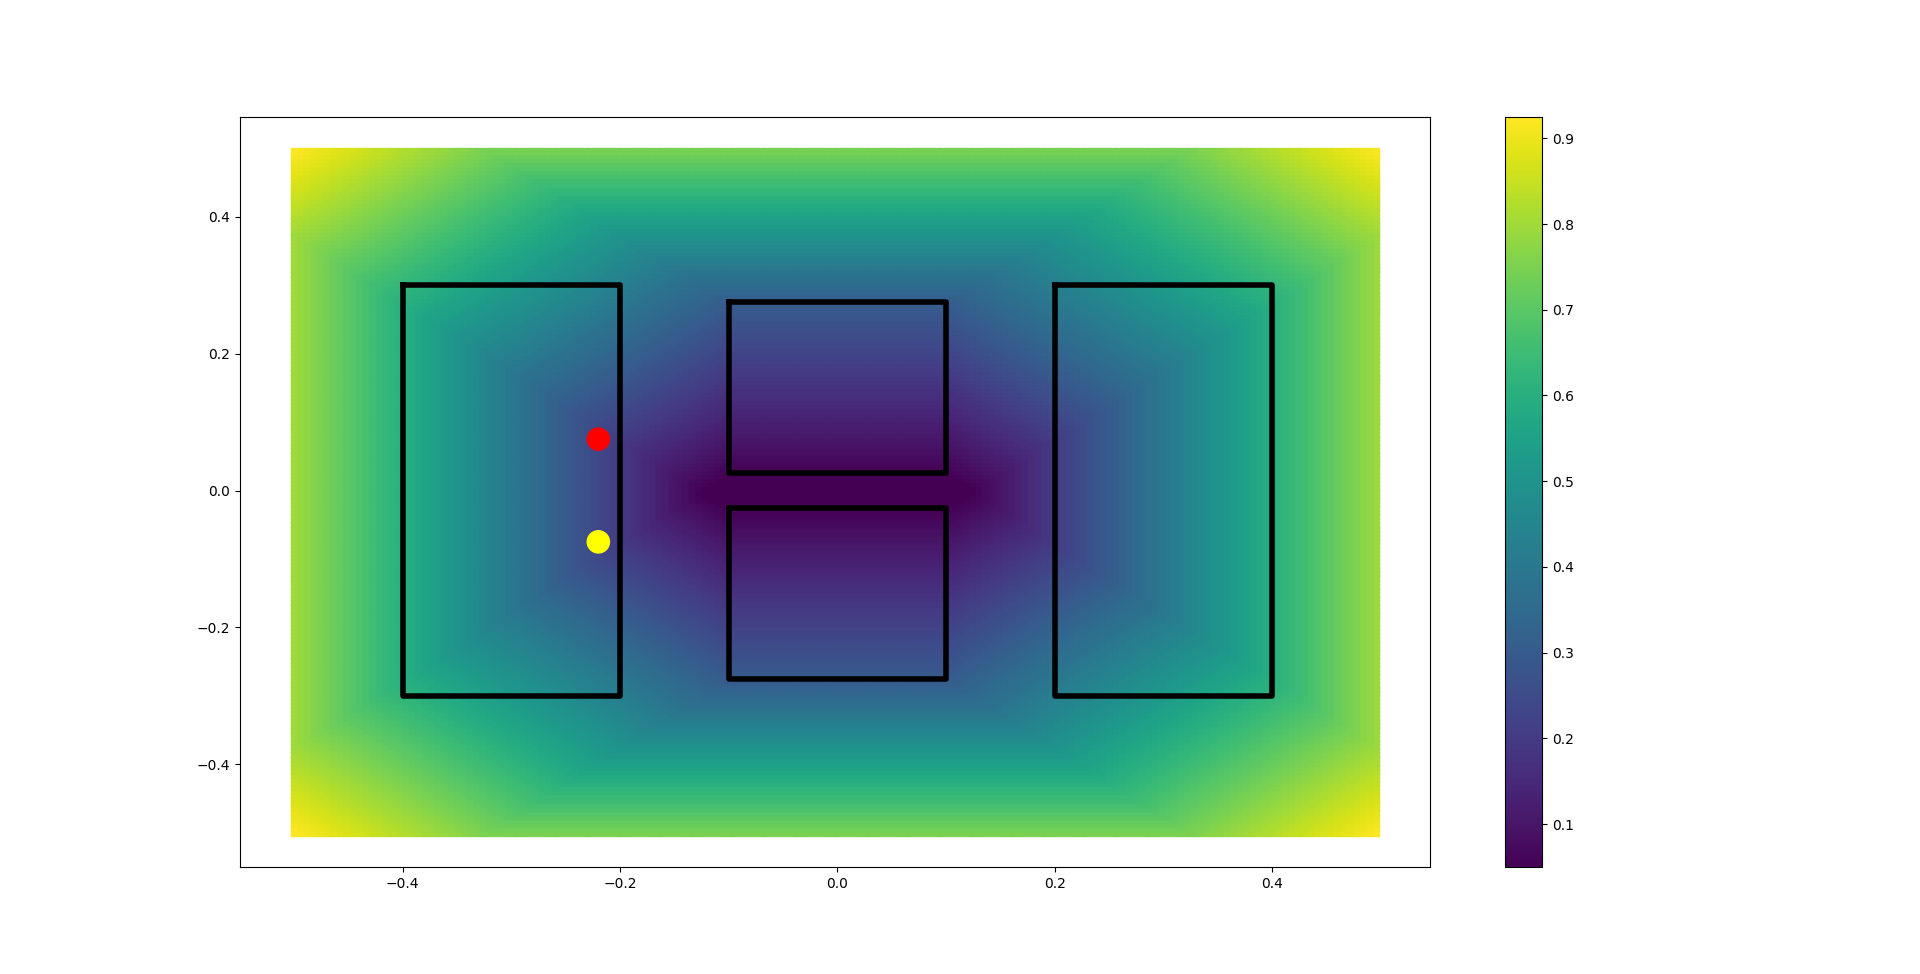
\includegraphics[trim={5cm 2cm 12cm 2cm},clip,width=\textwidth,height=4.5cm]{Figures/Chapter_MIP_SL1M/2_surf/scenario_0_init.png}};
        \draw (-0.25\textwidth, 0) node {\textbf{\textcolor{white}{1}}};
        \draw (0.01\textwidth, 0.6cm) node {\textbf{\textcolor{white}{2}}};
        \draw (0.01\textwidth, -0.6cm) node {\textbf{\textcolor{white}{3}}};
        \draw (0.28\textwidth, 0) node {\textbf{\textcolor{white}{4}}};
        % Points
        \draw (-0.22\textwidth, -0.45cm) node {\textbf{\textcolor{pink}{$p_1$}}};
    \end{tikzpicture}
    \caption{Initial foot placements.}
    \label{fig:sl1m:a11:0}
    \end{subfigure}
    \begin{subfigure}[t]{0.48\linewidth}
    \begin{tikzpicture}
        \draw (0, 0) node[inner sep=0] {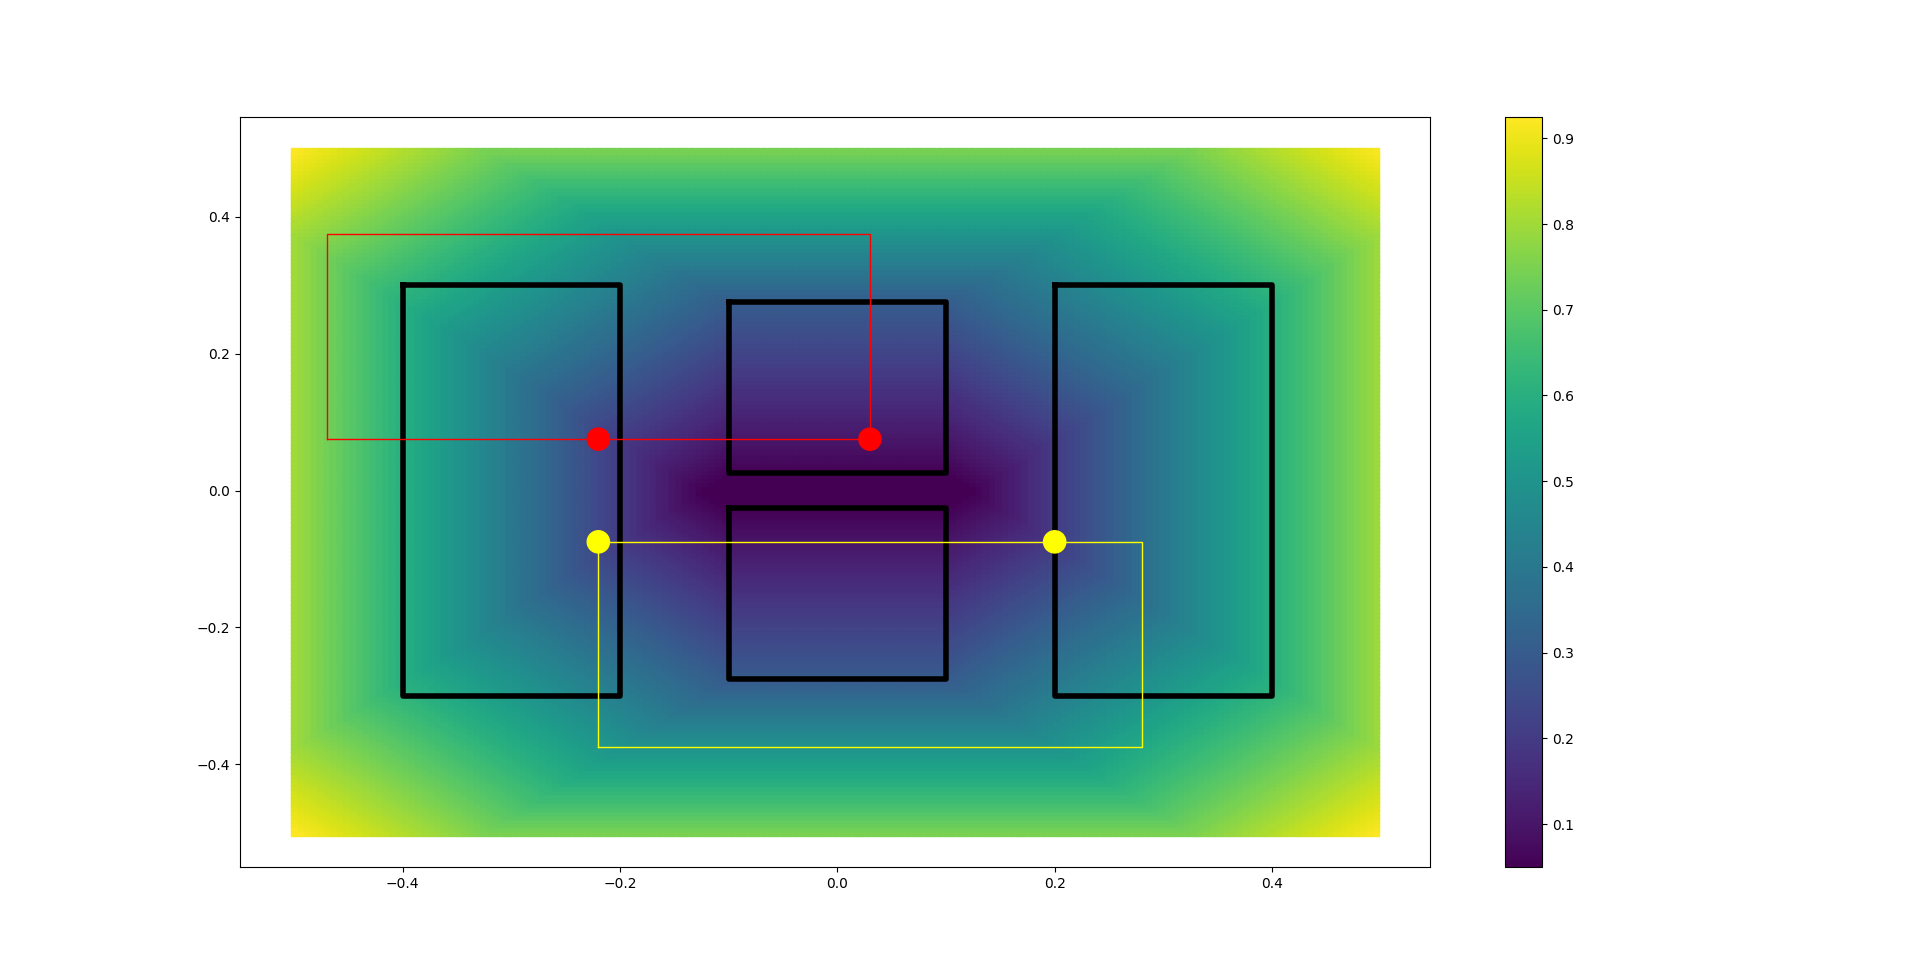
\includegraphics[trim={5cm 2cm 12cm 2cm},clip,width=\textwidth,height=4.5cm]{Figures/Chapter_MIP_SL1M/2_surf/scenario_0_constraint.png}};
        \draw (-0.25\textwidth, 0) node {\textbf{\textcolor{white}{1}}};
        \draw (0.01\textwidth, 0.6cm) node {\textbf{\textcolor{white}{2}}};
        \draw (0.01\textwidth, -0.6cm) node {\textbf{\textcolor{white}{3}}};
        \draw (0.28\textwidth, 0) node {\textbf{\textcolor{white}{4}}};
        % Points
        \draw (-0.22\textwidth, -0.45cm) node {\textbf{\textcolor{pink}{$p_1$}}};
        \draw (0.08\textwidth, 0.4cm) node {\textbf{\textcolor{pink}{p$_2$}}};
        \draw (0.2\textwidth, -0.55cm) node {\textbf{\textcolor{pink}{p$_3$}}};
    \end{tikzpicture}
    %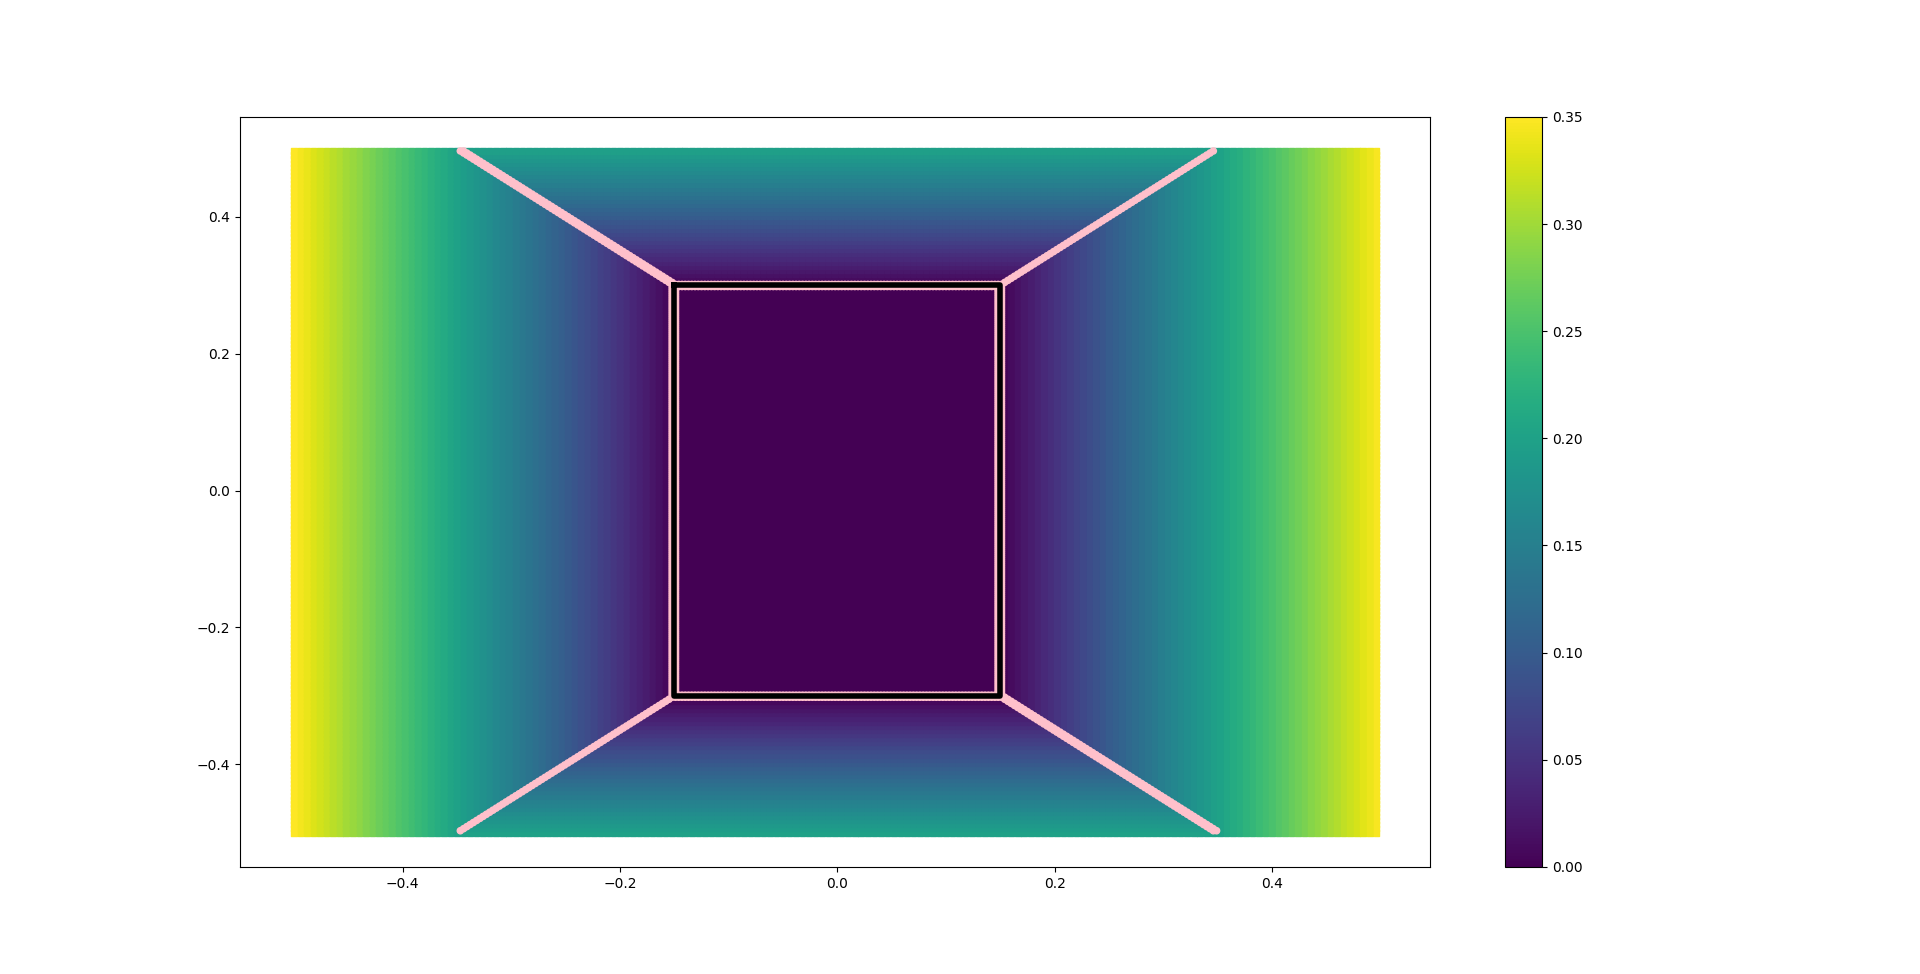
\includegraphics[trim={0 0 12cm 0},clip,width=\textwidth]{Figures/Chapter_MIP_SL1M/l1_no_cst/grad_simple_0_limit.png}
    \caption{Relaxed solution.}
    \label{fig:sl1m:a11:1}
    \end{subfigure}
    \caption{Scenario A.1: (red) left and (yellow) right feet. The robot has to perform two steps to reach surface $\mathcal{S}^4$.}
    \label{fig:sl1m:a11}
\end{figure}
% Other figure
\begin{figure}[ht]
    \centering
    \captionsetup[subfigure]{justification=centering}
    \begin{subfigure}[t]{0.48\linewidth}
    \begin{tikzpicture}
        \draw (0, 0) node[inner sep=0] {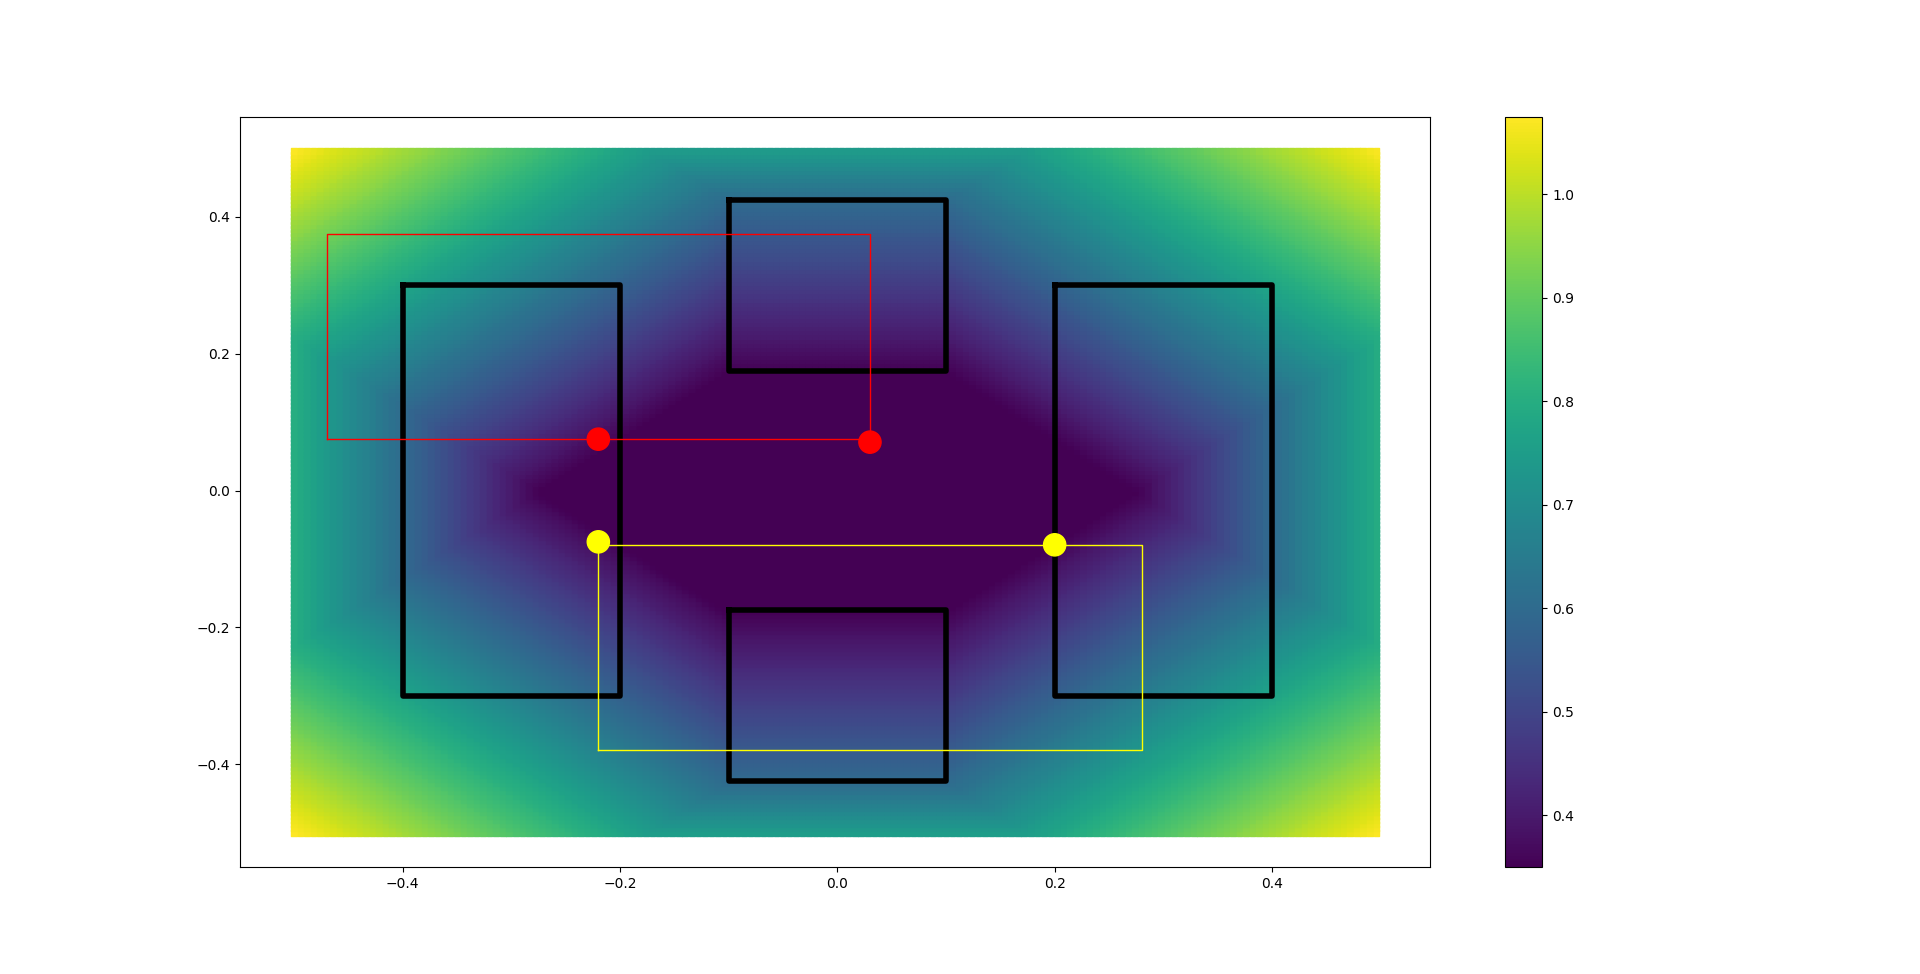
\includegraphics[trim={5cm 2cm 12cm 2cm},clip,width=\textwidth,height=4.5cm]{Figures/Chapter_MIP_SL1M/2_surf/scenario_0_problem.png}};
        \draw (-0.25\textwidth, 0) node {\textbf{\textcolor{white}{1}}};
        \draw (0.01\textwidth, 1.02cm) node {\textbf{\textcolor{white}{2}}};
        \draw (0.01\textwidth, -1.02cm) node {\textbf{\textcolor{white}{3}}};
        \draw (0.28\textwidth, 0) node {\textbf{\textcolor{white}{4}}};
        % Points
        \draw (-0.22\textwidth, -0.45cm) node {\textbf{\textcolor{pink}{$p_1$}}};
        \draw (0.08\textwidth, 0.4cm) node {\textbf{\textcolor{pink}{p$_2$}}};
        \draw (0.15\textwidth, -0.15cm) node {\textbf{\textcolor{pink}{p$_3$}}};
    \end{tikzpicture}
    %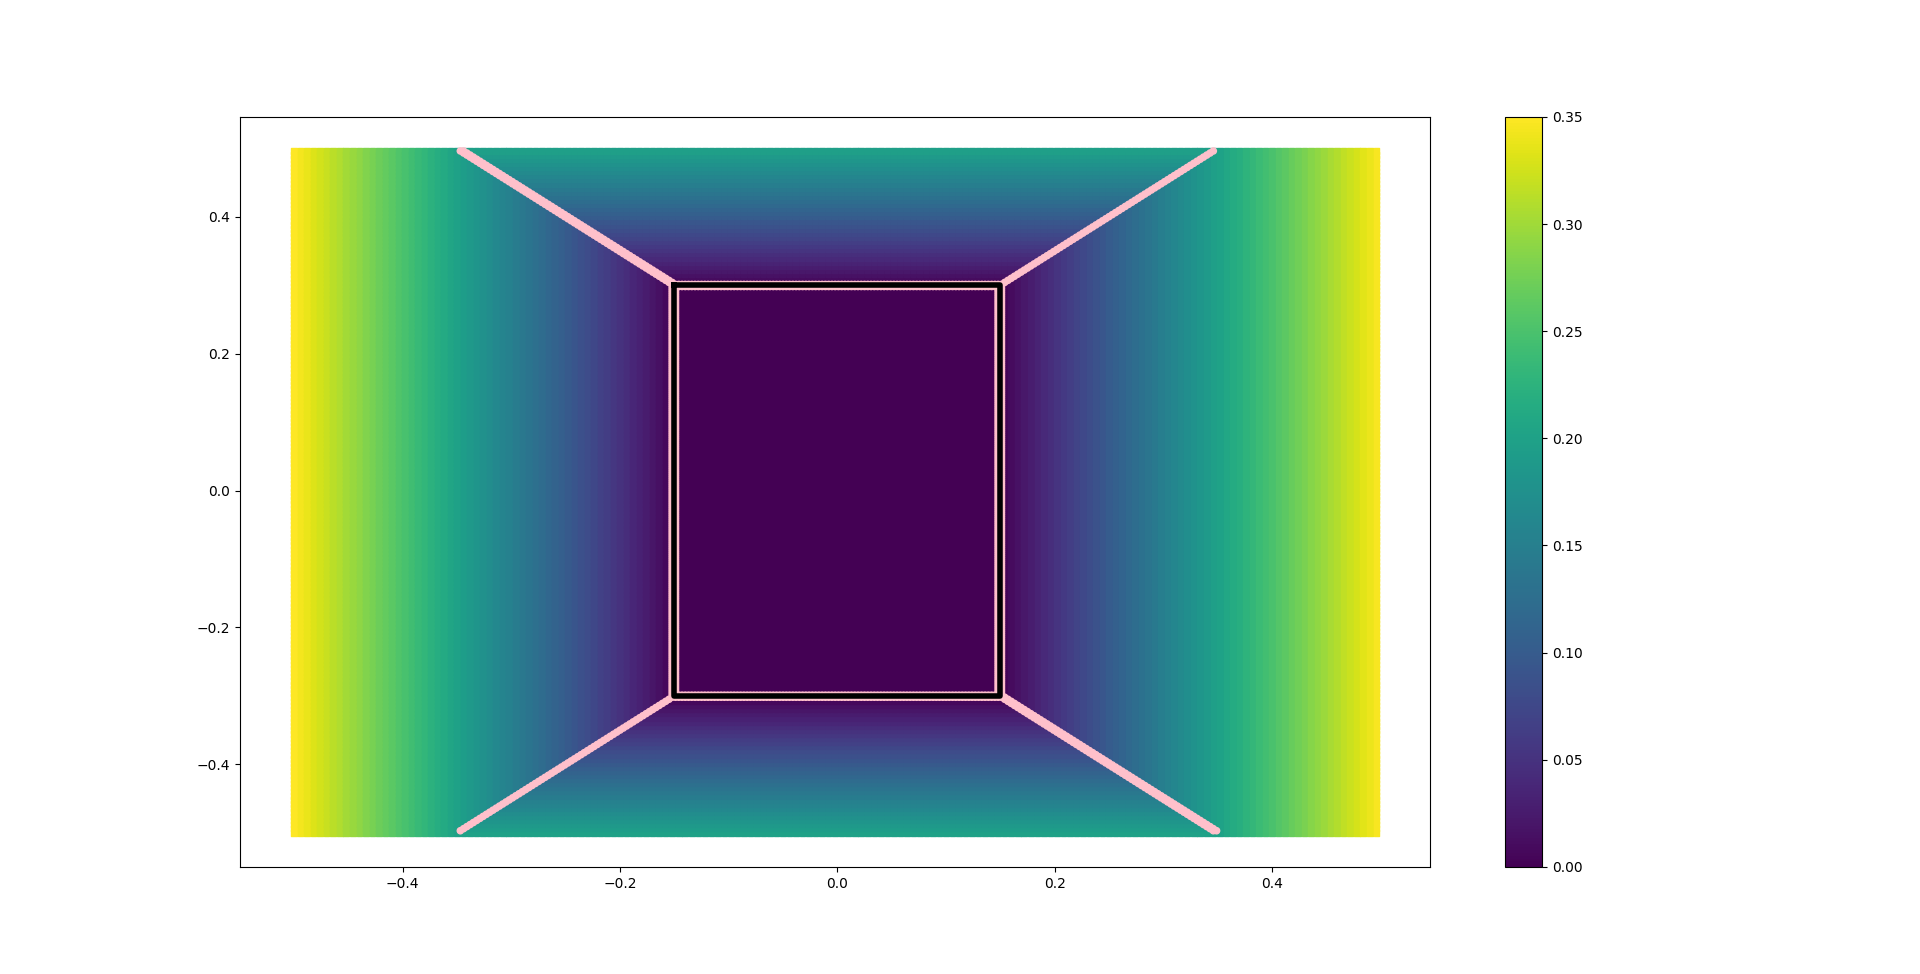
\includegraphics[trim={0 0 12cm 0},clip,width=\textwidth]{Figures/Chapter_MIP_SL1M/l1_no_cst/grad_simple_0_limit.png}
    \caption{Relaxed solution.}
    \label{fig:sl1m:a12:0}
    \end{subfigure}
    \begin{subfigure}[t]{0.48\linewidth}
    \begin{tikzpicture}
        \draw (0, 0) node[inner sep=0] {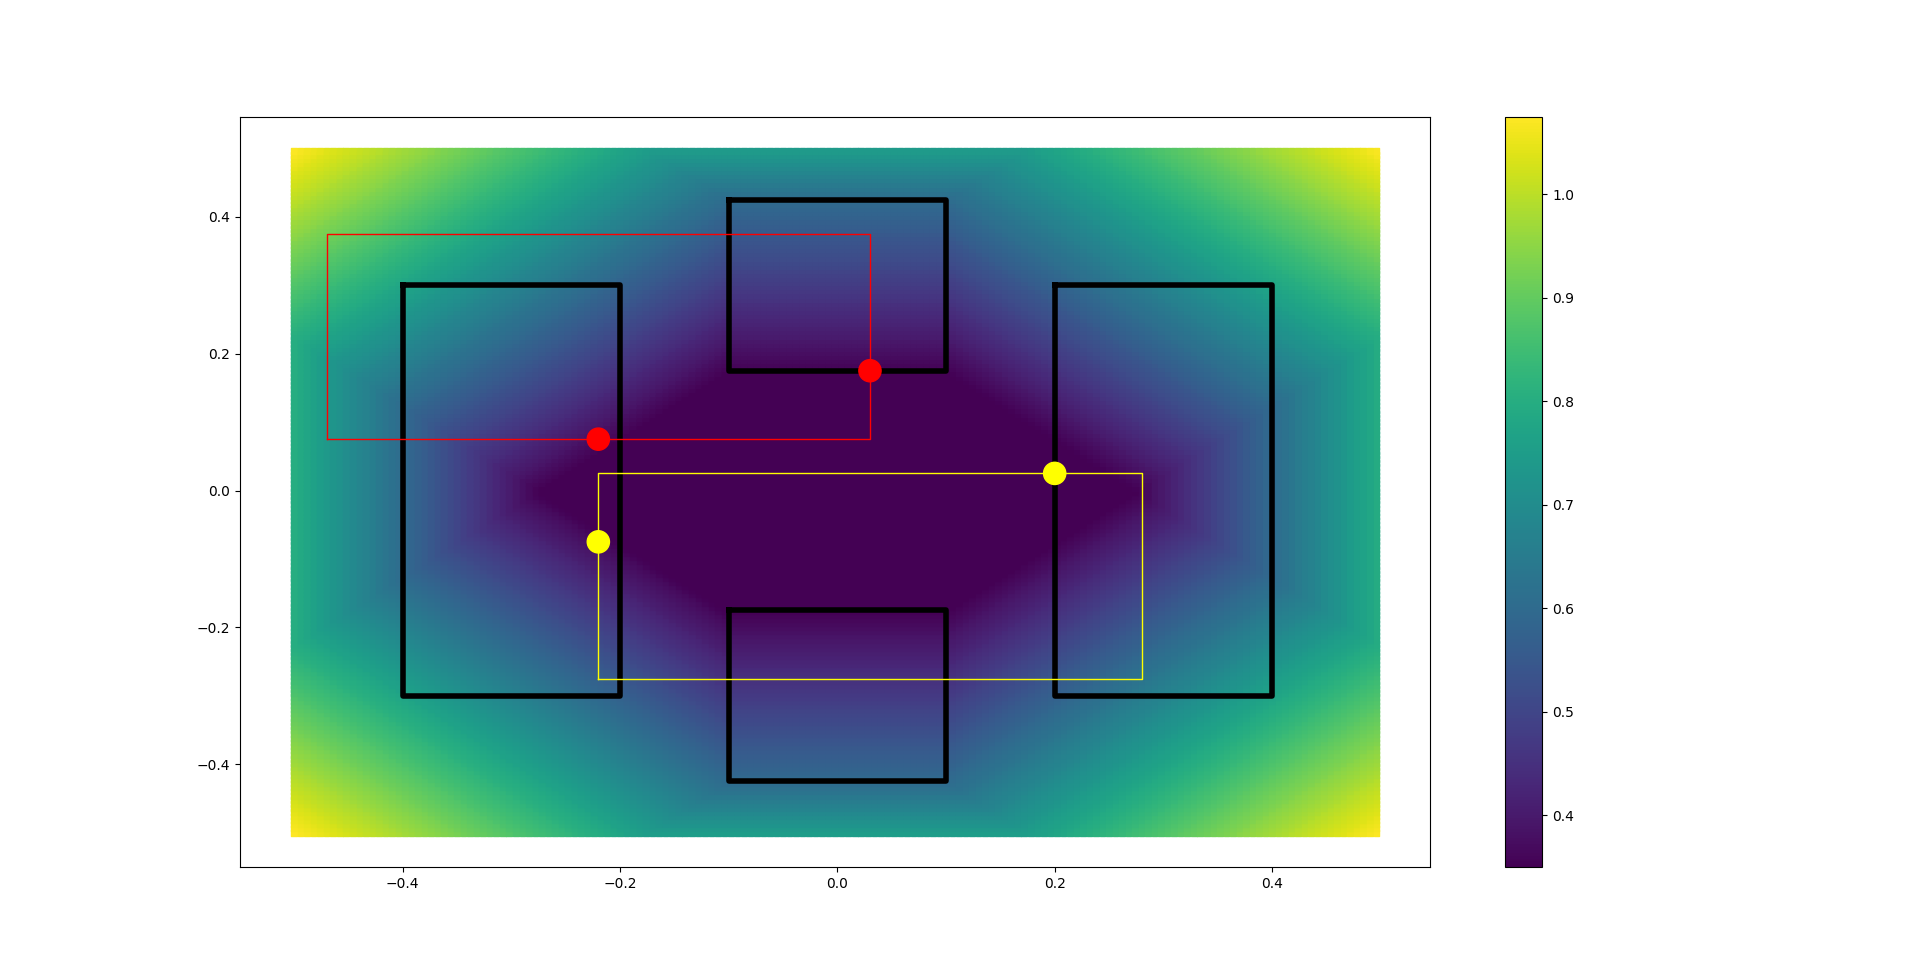
\includegraphics[trim={5cm 2cm 12cm 2cm},clip,width=\textwidth,height=4.5cm]{Figures/Chapter_MIP_SL1M/2_surf/scenario_0_problem_ok.png}};
        \draw (-0.25\textwidth, 0) node {\textbf{\textcolor{white}{1}}};
        \draw (0.01\textwidth, 1.2cm) node {\textbf{\textcolor{white}{2}}};
        \draw (0.01\textwidth, -1.2cm) node {\textbf{\textcolor{white}{3}}};
        \draw (0.28\textwidth, 0) node {\textbf{\textcolor{white}{4}}};
        % Points
        \draw (-0.22\textwidth, -0.45cm) node {\textbf{\textcolor{pink}{$p_1$}}};
        \draw (0.08\textwidth, 0.4cm) node {\textbf{\textcolor{pink}{p$_2$}}};
        \draw (0.15\textwidth, -0.15cm) node {\textbf{\textcolor{pink}{p$_3$}}};
    \end{tikzpicture}
    %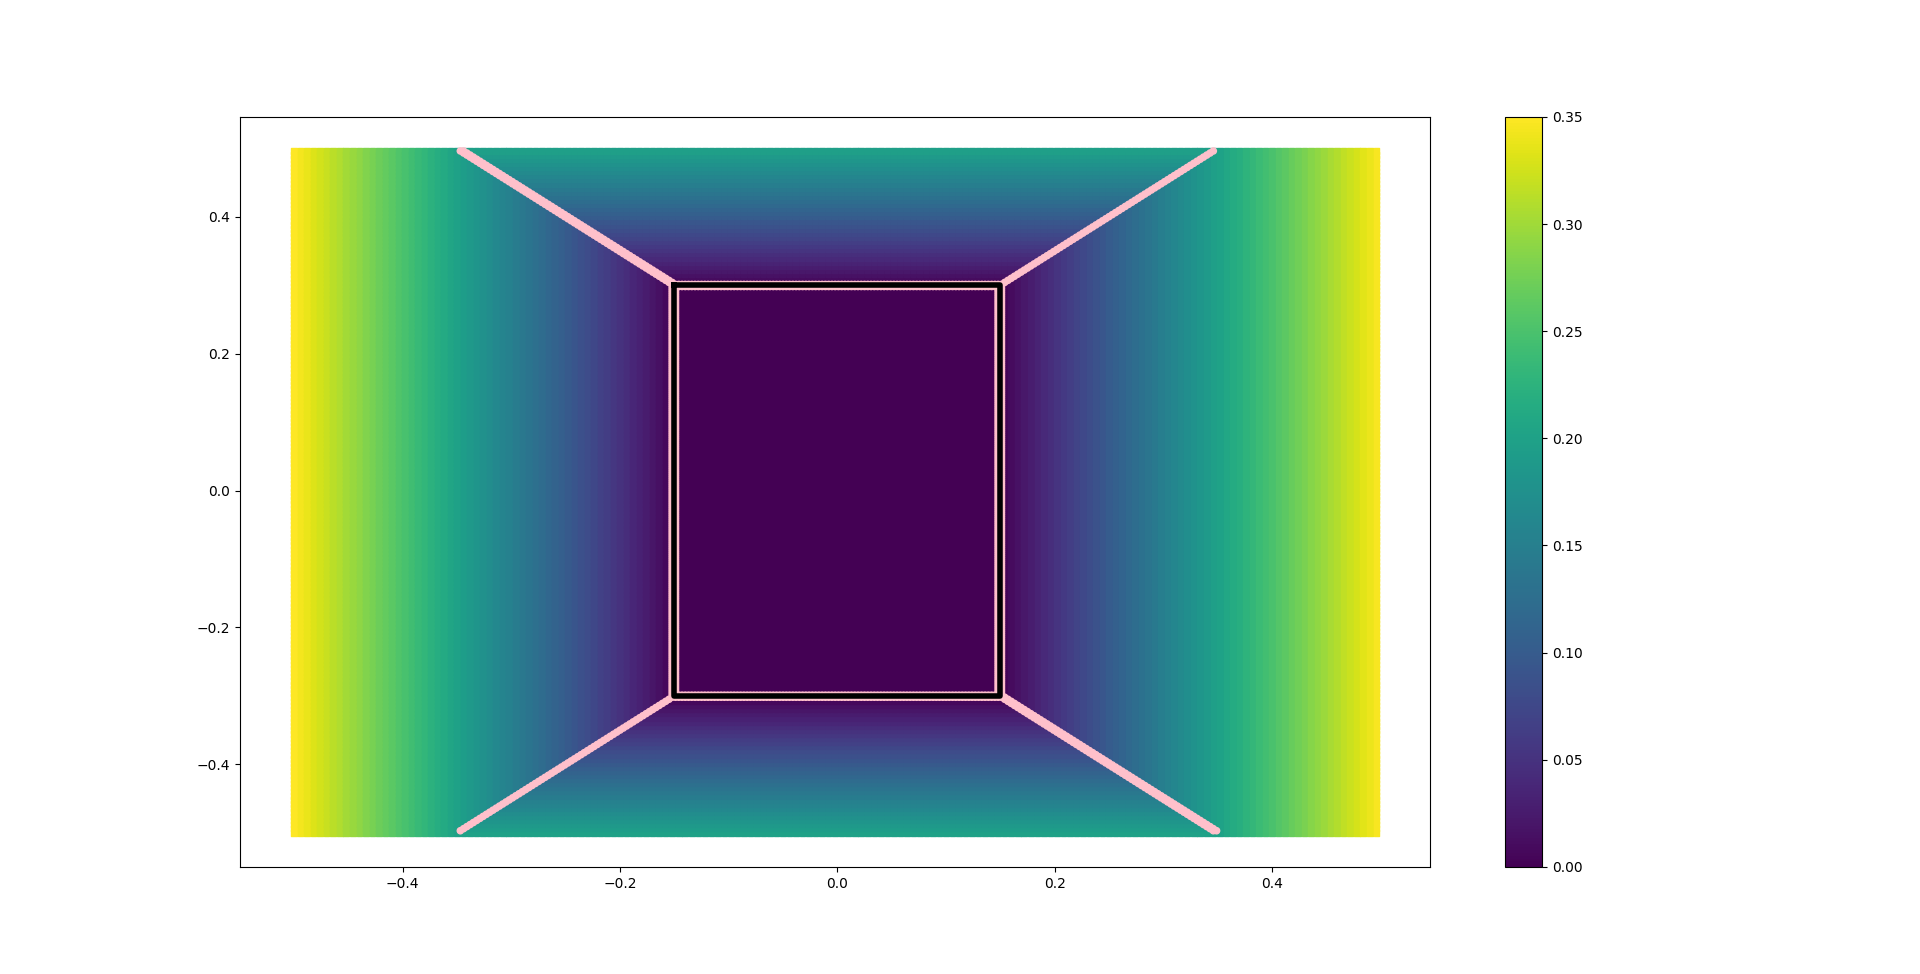
\includegraphics[trim={0 0 12cm 0},clip,width=\textwidth]{Figures/Chapter_MIP_SL1M/l1_no_cst/grad_simple_0_limit.png}
    \caption{With heuristics.}
    \label{fig:sl1m:a12:1}
    \end{subfigure}
    \caption{Scenario A.2: (a) the robot has to reach $\mathcal{S}^4$ in two steps, (b) SL1M does not solve the problem as p$_1$ does not lie on a surface, and (c) the heuristics succeeds the sub-problem with $\mathcal{S}^2$, the nearest surface to p$_1$.}
    \label{fig:sl1m:a12}
\end{figure}



\paragraph{Scenario B.}
As shown on figure \ref{fig:sl1m:final}, the robot has to cross a complex terrain composed of 10 surfaces and reach the surface $\mathcal{S}^{10}$ in 5 steps. 
We arbitrarily assign to each step position the following surface indices:
\begin{enumerate}
    \item $p_2 \; \Rightarrow$ \; $j = [1,2,3]$
    \item $p_3 \; \Rightarrow$ \; $j = [4,5]$
    \item $p_4 \; \Rightarrow$ \; $j = [4,5,6,7,8,9]$
    \item $p_5 \; \Rightarrow$ \; $j = [4,5,6,7,8,9]$
    \item $p_6 \; \Rightarrow$ \; $j = [10]$
\end{enumerate}
We plot 3 different $l1$-norm cost maps corresponding to the steps $\{p_2\}$, $\{p_3\}$, $\{p_4,p_5\}$ respectively.
As we can see, the cost map of $\{p_4,p_5\}$ contains higher values than the others as they have a lot more candidate surfaces. 
As a consequence, they will be more attracted toward their minimal cost area than the two others, p$_2$ and p$_3$ (Figure \ref{fig:sl1m:final:0}).

In this scenario, SL1M selects some surfaces for $p_2 \in \mathcal{S}^2$, $p_3 \in \mathcal{S}^5$, and obviously $p_6 \in \mathcal{S}^{10}$ that is a hard constraint. 
However, it does not solve the problem as $p_4$ and $p_5$ do not belong to any surface.
As a consequence, the heuristics generates 36 sub-problems as $p_4$ and $p_5$ can potentially lie on 6 different surfaces each. 
By testing all lowest cost combinations first, the heuristics finds a feasible solution after 5 explorations (Figure \ref{fig:sl1m:final:1}).

\begin{figure}[h!]
    \centering
    \captionsetup[subfigure]{justification=centering}
    \begin{subfigure}[t]{0.9\linewidth}
        \begin{tikzpicture}
            \draw (0, 0) node[inner sep=0] {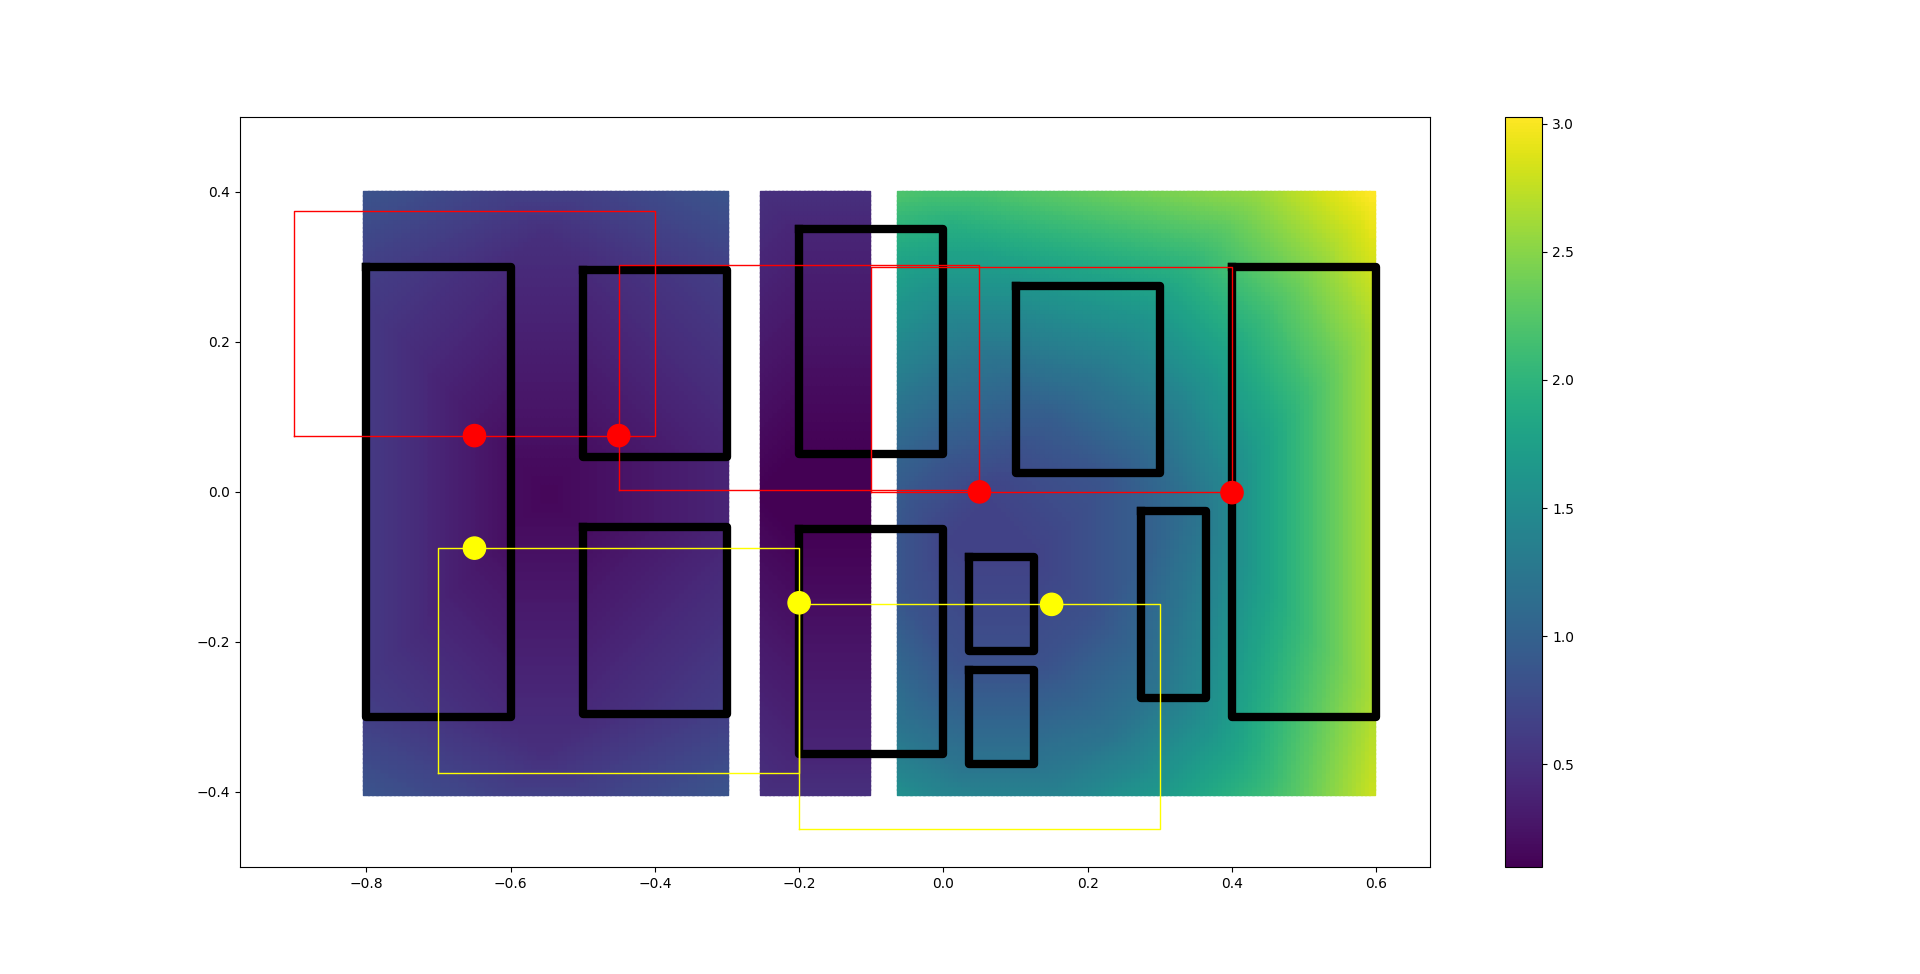
\includegraphics[trim={2cm 2cm 7cm 2cm}, clip,width=\textwidth,height=7cm]{Figures/Chapter_MIP_SL1M/sl1m_final/final_sl1m_2_better.png}};
            % Names surfaces
            \draw (-0.27\textwidth, 0cm) node {\textbf{\textcolor{white}{1}}};
            \draw (-0.13\textwidth, 1.21cm) node {\textbf{\textcolor{white}{2}}};
            \draw (-0.13\textwidth, -1.21cm) node {\textbf{\textcolor{white}{3}}};
            \draw (-0.015\textwidth, 1.3cm) node {\textbf{\textcolor{white}{4}}};
            \draw (-0.015\textwidth, -1.34cm) node {\textbf{\textcolor{white}{5}}};
            \draw (0.09\textwidth, -0.96cm) node {\textbf{\textcolor{white}{6}}};
            \draw (0.09\textwidth, -1.95cm) node {\textbf{\textcolor{white}{7}}};
            \draw (0.145\textwidth, 1cm) node {\textbf{\textcolor{white}{8}}};
            \draw (0.2\textwidth, -0.8cm) node {\textbf{\textcolor{white}{9}}};
            \draw (0.28\textwidth, 0cm) node {\textbf{\textcolor{white}{10}}};
            % Points
            \draw (-0.27\textwidth, -0.75cm) node {\textbf{\textcolor{pink}{$p_1$}}};
            \draw (-0.175\textwidth, 0.65cm) node {\textbf{\textcolor{pink}{p$_2$}}}; % P1
            \draw (-0.015\textwidth, -0.8cm) node {\textbf{\textcolor{pink}{p$_3$}}}; % P2
            \draw (0.095\textwidth, 0.195cm) node {\textbf{\textcolor{pink}{$p_4$}}}; % P3
            \draw (0.145\textwidth, -0.75cm) node {\textbf{\textcolor{pink}{$p_5$}}}; % P4
            \draw (0.215\textwidth, 0.1cm) node {\textbf{\textcolor{pink}{$p_6$}}}; % P5
        \end{tikzpicture}
        \caption{Relaxed solution.}
        \label{fig:sl1m:final:0}
    \end{subfigure}
    \begin{subfigure}[t]{0.9\linewidth}
        \begin{tikzpicture}
            \draw (0, 0) node[inner sep=0] {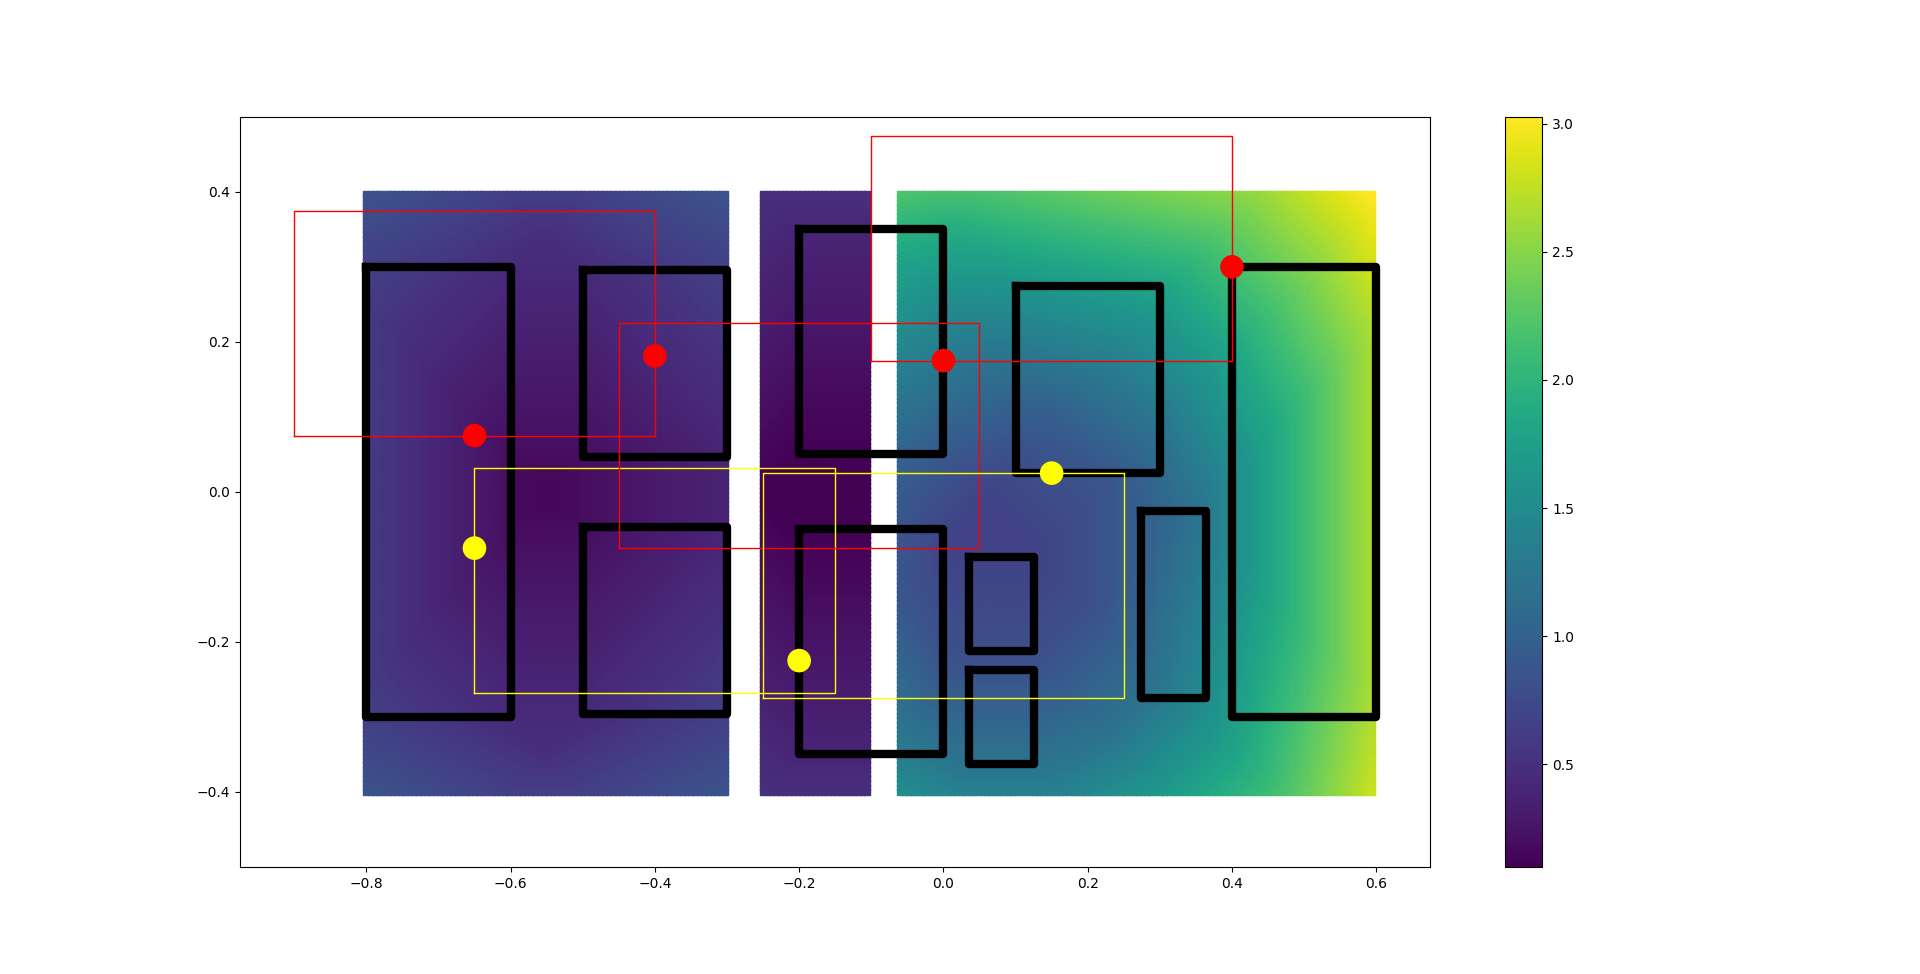
\includegraphics[trim={2cm 2cm 7cm 2cm}, clip,width=\textwidth,height=7cm]{Figures/Chapter_MIP_SL1M/sl1m_final/final_sl1m_2_better_heuristics.png}};
            % Names surfaces
            %\draw (-0.27\textwidth, 0cm) node {\textbf{\textcolor{white}{1}}};
            %\draw (-0.13\textwidth, 1.21cm) node {\textbf{\textcolor{white}{2}}};
            %\draw (-0.13\textwidth, -1.21cm) node {\textbf{\textcolor{white}{3}}};
            %\draw (-0.015\textwidth, 1.3cm) node {\textbf{\textcolor{white}{4}}};
            %\draw (-0.015\textwidth, -1.34cm) node {\textbf{\textcolor{white}{5}}};
            %\draw (0.09\textwidth, -0.96cm) node {\textbf{\textcolor{white}{6}}};
            %\draw (0.09\textwidth, -1.95cm) node {\textbf{\textcolor{white}{7}}};
            %\draw (0.145\textwidth, 1cm) node {\textbf{\textcolor{white}{8}}};
            %\draw (0.2\textwidth, -0.8cm) node {\textbf{\textcolor{white}{9}}};
            %\draw (0.28\textwidth, 0cm) node {\textbf{\textcolor{white}{10}}};
            % Points
            \draw (-0.27\textwidth, -0.75cm) node {\textbf{\textcolor{pink}{$p_1$}}};
            \draw (-0.115\textwidth, 0.85cm) node {\textbf{\textcolor{pink}{p$_2$}}}; % P1
            \draw (-0.015\textwidth, -1.25cm) node {\textbf{\textcolor{pink}{p$_3$}}}; % P2
            \draw (0.039\textwidth, 0.8cm) node {\textbf{\textcolor{pink}{$p_4$}}}; % P3
            \draw (0.145\textwidth, 0.285cm) node {\textbf{\textcolor{pink}{$p_5$}}}; % P4
            \draw (0.22\textwidth, 1.6cm) node {\textbf{\textcolor{pink}{$p_6$}}}; % P5
        \end{tikzpicture}
        \caption{With heuristics.}
        \label{fig:sl1m:final:1}
    \end{subfigure}
    \caption{Scenario B: (a) SL1M does not solve the problem for $p_4$ and $p_5$, and (b) the heuristics finds a solution after 5 combinatorial explorations. We plot 3 different $l1$-norm cost maps for $\{\mbox{p}_2\}$, $\{\mbox{p}_3\}$ and $\{\mbox{p}_4,\mbox{p}_5\}$ respectively.}
    \label{fig:sl1m:final}
\end{figure}

\subsection{Problem Statement}
SL1M formulation is promising to solve the contact planning problem with a simple linear optimization solver.
We have seen that the $l1$-norm cost encourages the sparsity among the slack variables $\alpha_i$ for each step, and so the selection of surfaces.
%However, the formulation of the problem comes with limitations depending on the terrain geometry.

SL1M outputs foot positions that are attracted toward their minimal cost area formed by their candidate surfaces.
As the cost gradients generally operate at the edges of surfaces, the foot positions are encouraged to lie on them.
In synergy with the foot constraints as well as the cost balancing between each step, it permits to find a sufficient approximation in our test scenarios.

However, we have also seen that SL1M rarely solves the problem directly. 
It often requires the use of heuristics to explore the combinatorics for undecided steps, which can grow exponentially with the number of footsteps and surface candidates \cite{sl1m_v1}.

Moreover, the heuristics presently used can lead to unfeasible problems. 
Indeed, fixing selected surfaces in the SL1M solution further constrains our set of possibilities. While lowering the combinatorics to explore, it can also lead to unfeasible sub-problems. As a consequence, we may lose the guarantee of completeness.
At the moment, we do not have better heuristics or solutions other than the branch-and-bound algorithm to fix this limitation.

Another important remark is that the constraints have been simplified in the previous examples.
The full set of kinematic and dynamic constraints $\mathcal{F}$ (Appendix \ref{appendix:feasibility_constr}) further reduces the feasibility spaces, which irremediably makes the combinatorial exploration with the heuristics less likely to succeed.
%\textcolor{red}{Steve: ??? plus tu contrains, plus t'as de chance que ca converge.} \textcolor{blue}{Pas vraiment... Exemple sur un de mes scenarios avec les debris: (a) SL1M sans contrainte sur le COM = 19 succes sur 20 tests, et (b) avec contraintes 17/20.*
%Comme tu fixes des surfaces avec l'heuristics, t'as des chances qu'elle rende le probleme totalement infaisable. Si en plus tu mets encore plus de contraintes de faisabilité, tu vas encore plus echouer. C'est pour ça que je t'ai posé la question sur les slack à l'intérieur des contraintes de faisabilité. Je pensais qu'elles pouvaient potentiellement aider ce probleme?}

To fix these limitations, we explore a lead from the previous work \cite{sl1m_v2}, that is the impact of the guide path and its discretization on the SL1M problem.
In their result, they notice that its tuning is critical to generate easier SL1M problems.
Indeed, as shown in the previous section on MIP, we need sufficiently small discretization steps $\Delta D$ for the problem to be feasible. 
However, SL1M introduces a new dimension to the problem with its formulation, in regard to the $l1$-norm.
We thus conduct several experiments to answer the following question: \textit{Can we generate guide paths further helping SL1M relaxation?}


\subsection{Experiments Conducted and Discussion}
% What did I do ?
% - Adapt the velocity for MIP => ok. Solution sparse + Solution MPC (and why PBP not good). Explain why. => Ok it worked.
% - Check the success rate of SL1M with the same approach. => It did not work, you can guess why from the insight.
% - Ideas explored for SL1M =>  Reduce the number of surfaces.
%                               Select less but more probable surfaces (the heuristics I did).
%                               Effect of having more or less steps?
%                               Adding some weights on the surfaces (This is more an experiment, use the map I did for that).

We aim to increase the success rate of SL1M contact planner, with as little combinatorial exploration as possible using the heuristics.
This objective is also related to the work in the previous Section \ref{subsub:mip:implementation_details}. 
Indeed, if a problem is not feasible by the MIP contact planner, then it is not feasible by SL1M, its relaxed form.
To achieve this objective, we tested the exact same approaches we had with LEAS and the other contact planners.

\paragraph{Testing our previous approaches.}
%First, we employed the strategy of the sampling based contact planner (Section \ref{sec:CP-SB}).
First, we trained LEAS to follow a desired velocity $v_{desired}=0.10$ m/s. 
Then, we aimed for an average discretization step $\Delta D=20$ cm along the guide given to SL1M, value for which MIP contact planning is nearly always feasible (See Section \ref{subsub:mip:results}).
LEAS-P2 was trained for two modes, with and without feedback from SL1M. Just as with the MIP contact planner, we perform a dichotomic search of the last successful step along the guide, feedbacked during the training.
However, this experiment was not successful as both RL policies did not converge.
In our training area, the policy was making the robot idle on flat ground to accumulate positive rewards, without crossing any transition tile. 
Indeed, the policy deemed the transition tiles (rubbles, stairs, bridge) too difficult to be crossed with the contact planner SL1M for both modes.
As a result, it preferred staying idle on flat ground with only one candidate surface on it per step, the flat ground surface under the robot.
This strategy thus avoids the difficulty of SL1M contact planning and does not permit us to achieve our navigation task.


\paragraph{Sanity check with a sparse reward.}
To force LEAS in confronting both the navigation task and SL1M contact planning, we performed a sanity test on the stairs scenario.
To do so, LEAS-P2 was trained with a simple sparse reward:
\begin{equation}
    R = \left\{
    \begin{array}{ll}
        1 & \mbox{if objective reached with P1 and SL1M}\\
        0 & \mbox{otherwise}\\
    \end{array}
\right.
\end{equation}
In order to maximize the episode reward, LEAS is thus forced to succeed in climbing the stairs with the contact planner.

With the heuristics, the steering methods with SL1M achieve similar results to the MIP contact planner on stairs (\ref{subsub:mip:basic_scenarios}).
That is why in this simple scenario, we performed it without its heuristics to analyze the direct impact of the guide on the relaxation.
%With the heuristics, SL1M always succeeds on scenarios with a small number of steps \cite{sl1m_v1}.
%However, to achieve our objective, we wanted to analyze the impact of the guide discretization on the relaxation itself without the heuristics.
As LEAS-P2 rarely reaches the objectives with the following reward, the network was pretrained using trajectories generated by LEAS-P1 to guide its exploration.
We increased the discount factor $\gamma$ from $0.97$ to $0.995$ to encourage LEAS-P2 in reaching the objective with SL1M in the least feasible number of steps, without modifying the sparse reward.

After training, we observed some improvements in SL1M success rate, but with unexpected behavior.
LEAS-P2 was making the robot sidewalk at the maximum feasible discretization step (when sidewalking) up to the objective.
This result correlates with our previous experiment on the sampling-based contact planner (Chapter \ref{sec:CP-SB}), where sidewalking is a preferred walking strategy in regard to the robot equilibrium constraints.

To avoid sidewalking behavior, we thus forced the robot orientation toward the goal.
After training, the success rate was lower than without the orientation enforcement.
The policy learned that the best strategy was to reach the target in the least number of steps possible.
This strategy makes sense as by reducing the size of the problem, we possibly reduce the number of footsteps not lying on a surface.
However, it was not the results we expected, and we did not see any other meaningful behavior.

\paragraph{Conclusion and Prospective}

Our experiments on SL1M with LEAS were not successful.
The guide path does impact the problem to solve, but its control over it is limited.
%\textcolor{blue}{Montrer rubbles MIP vs SL1M without heuristics vs SL1M with heuristics}

LEAS can not accurately select the candidate surfaces for each step. However, those are at the core of SL1M formulation (Section \ref{subsub:insight_l1}). 
Indeed, each problem is characterized by the number of steps, as well as the number and geometry of candidate surfaces for each step.
In addition to optimizing the discretization step along the guide for a solution to exist, the SL1M solution is also much more dependent on the past trajectory compared to the MIP contact planner.

As previously discussed, LEAS is not aware of the past trajectory and candidate surfaces when controlling the robot root. 
In its actual state, LEAS can generate feasible problems. However, it can not further help SL1M formulation.
An approach could be to investigate the use of recurrent neural networks in LEAS to permit an internal representation of this past trajectory.

However, we believe that helping to solve SL1M with the guide path may not be the right approach to the problem.
Indeed, we may have to investigate the formulation itself.
An idea could be to add weights to the slack variables in function of the surface probability to be stepped on.
This way, the $l1$-norm minimal area would be more attracted toward these surfaces. 
However, it is difficult problem to decide how to assign these weights, and machine learning could be useful for it.

In future work, further exploring how to improve this formulation is an exciting direction. 
Finally, this also encompasses a broader range of applications not specific to contact planning which all aim to solve more efficiently Mixed-Integer Programming problems.